\documentclass[12pt]{article}
\usepackage{graphicx}
% \graphicspath{{/Users/justindoty/Desktop/QPF/Figures/}}
\graphicspath{{/Users/justindoty/Documents/Research/Dissertation/Production_QR_Proxy/Code/Figures/}}
% \graphicspath{{/Users/suysong/Dropbox/AAA_Song/Research/JustinDoty/QuantileProductionFunction/text/Figures/}}
\usepackage{graphics}
\usepackage{amsfonts}
\usepackage{amsmath}
\usepackage{amstext}
\usepackage{tabularx}
\usepackage{mathrsfs}
\usepackage{subfigure}
\usepackage[dvipsnames]{xcolor}
\usepackage{lscape}
\usepackage{longtable}
\usepackage{bm}
\usepackage{bbm}
\usepackage{chngcntr}
\usepackage{setspace}
\usepackage{caption}
\usepackage{float}
\usepackage{multirow}
\usepackage{appendix}
\usepackage{booktabs}
\usepackage{natbib}
\usepackage{fancyvrb}
\usepackage{enumitem}
\usepackage[multiple]{footmisc}
\newtheorem{assump}{Assumption}[section]
\newtheorem{lemma}{Lemma}[section]
\newtheorem{corollary}{Corollary}[section]
\newtheorem{theorem}{Theorem}[section]
\newcommand{\indep}{\perp \!\!\! \perp}


\usepackage[multiple]{footmisc}

%Set margins and text size
\setlength{\textwidth}{6.5in} \setlength{\textheight}{8.8in}
\setlength{\topmargin}{-0.5in}
\setlength{\oddsidemargin}{-0.01in}{}
\setlength{\parskip}{1.6mm}
\parskip=.06in
{}
%Some useful short-cuts
\def\argmax{\mathop{\rm arg\,max}}
\def\argmin{\mathop{\rm arg\,min}}



\setcounter{section}{0} % starts numbering section 1start_value=[0.498,-0.2874,0.4314,0.5444];

\setcounter{page}{1}



\usepackage{hyperref}
\hypersetup{
    colorlinks=true,
    allcolors=Violet
}
\begin{document}

\title{Estimating Quantile Production Functions: \\
A Control Function Approach}

\author{Justin Doty\thanks{Department of Economics, University of Iowa, S321 Pappajohn Business Building, 21 E Market St, Iowa City, IA 52242. Email: \href{mailto:justin-doty@uiowa.edu}{\texttt{justin-doty@uiowa.edu}}} and Suyong Song\thanks{Department of Economics and Finance, University of Iowa, W360 Pappajohn Business Building, 21 E Market St, Iowa City, IA 52242. Email: \href{mailto:suyong-song@uiowa.edu}{\texttt{suyong-song@uiowa.edu}}}
}

\date {\today}
\maketitle


\begin{abstract}
We propose a new approach to estimate production functions in which output elasticities are heterogeneous across the conditional distribution of output. This paper extends the control function approach for estimating production functions to the conditional quantiles of firm production. Production function parameters are estimated in a simple two-stage approach which relies a location-shift assumption on unobserved productivity. We show that this method allows us to capture heterogeneity in output elasticities that may not be found in conditional mean estimates of \cite{Ackerberg2015} or \cite{Levinsohn2003}. We provide small-sample evidence in a Monte Carlo study to show that this approach is robust compared to other production function estimators. The method is applied to firm and plant-level manufacturing data from the U.S., Chile, and Colombia. The findings confirm that the proposed method captures unobserved heterogeneity in output elasticities.
\end{abstract}


\textit{Keywords:} Production functions, heterogeneous elasticity, quantile regression

\textit{JEL Classification:} C14, C36, D24


\pagenumbering{arabic}

\baselineskip25pt

%\singlespacing
\onehalfspacing
%\doublespacing

\section{Introduction}

Production function estimation is an ongoing and historical empirical research topic that links firm's input to output decisions. Identification of the output elasticities and consequently the distribution of firm-level productivity is constrained by endogeneity issues. This is because productivity is unobserved by the econometrician, but observed by the firm when making input decisions. 

A popular approach to address this issue is to introduce a proxy variable such as investment, made popular by \cite{Olley1996} (OP) or an intermediate input using \cite{Levinsohn2003} (LP) or \cite{Ackerberg2015} (ACF). These proxies are functions of a state variable such as capital and unobserved productivity. Under certain assumptions, this function is strictly increasing in its scalar unobserved productivity component. Inverting this function controls for unobserved productivity and the production function parameters can be estimated with a simple two-stage estimator.

Model specification is an important issue for production function estimation. Estimates may be biased if there is additional heterogeneity in production technology across firms that are not captured by traditional approaches. More flexible models could reduce productivity heterogeneity which affects subsequent analysis of it using firm characteristics such as exporting or R\&D activity. Allowing for heterogeneous coefficients is one possible way to capture these differences. The literature on heterogeneous production functions is small relative to the empirical research using the homogeneous coefficient model, even though many recent empirical studies have found heterogeneity in firm behavior and decisions.\footnote{Some notable examples are \cite*{Kasahara2015}, \cite*{balat} and \cite*{Li2017} to name of few. Also \cite{Gandhi2020} who estimate a nonparametric production function and obtain heterogeneous estimates.} This is because estimating the homogeneous coefficient model by itself is very difficult due to the issue of unobserved productivity. Moreover, production function estimators that use conditional mean estimates are less robust to outliers than conditional quantile estimates. In this circumstance, the conditional median may be more appropriate for any analysis that relies on estimates of output elasticities, for example returns to scale, capital intensity, or total factor productivity (TFP). Even in situations where median estimates are similar to the mean, quantile regression estimates give a richer description of the entire conditional distribution of output. Therefore, we propose a quantile regression framework for estimating production functions, while also controlling for the simultaneity issue of unobserved productivity.  

The literature on control function approaches for quantile regression models is still a developing area. Therefore, it is not straightforward to estimate production functions by allowing for endogenous inputs and their heterogeneous coefficients.\footnote{See for example \cite{Chesher2003}, \cite{Ma2006}, and \cite{Lee2007}.} This is likely due to the fact that the control function approaches of OP, LP, and ACF rely on conditional moment restrictions on multiple unobservables. For example, the second stage of their approach utilizes the condition $\mathbbm{E}[\xi_{it}+\varepsilon_{it}|\mathcal{I}_{it-1}]=0$ where $\xi_{it}$ are innovations to productivity, $\varepsilon_{it}$ are independent and identically distributed (i.i.d.) ex-post shocks to production, and $\mathcal{I}_{it-1}$ is the firm's information set at time $t-1$. This restriction does not extend naturally to conditional quantiles, since unlike expectation operators, quantile operators are non-linear. In contrast to the mean of multidimensional unoservables, there is no consensus about defining the quantile counterpart. As a result, it is a non-trivial task to appropriately define quantile functions in the presence of bivariate unobservables, $\xi_{it}$ and $\varepsilon_{it}$, in the conventional framework of the control function approaches. Similar issues are encountered in the quantile panel data literature where researches have proposed alternatives to individual fixed effects using correlated random effects.\footnote{See for example \cite{Harding2016} and \cite{Cai2018} for two separate approaches.} However, these approaches are not directly applicable to estimating the conditional quantiles of production functions, since the unobservables in production functions are typically assumed to be time-varying.

In our model, we allow for non-neutrality of the unobserved idiosyncratic production shock, while the component of productivity that is anticipated by firms to be Hicks-neutral.  We use the control function approach in this framework in order to control for the part of production unobservables that are correlated with input decisions. We are not aware of any published paper which takes into account the endogeneity issue of production functions in the conventional quantile regression framework. We fill the gap in this paper by proposing an easy-to-implement estimator which is available on the author's \href{https://github.com/justdoty/Quantile-Production-Functions}{Github}. 

We show the conditional quantiles of firm production are non-parametrically identified using conditional deconvolution arguments under independence of the unobservable technology shocks, productivity, and productivity innovation shocks conditional on inputs and other mild regularity conditions on the conditional characteristic functions. These assumptions are plausible and have been used in identification arguments of other work such as \cite{Hu2019}. The conditional characteristic functions are identified up to a location normalization. We show that using the conditions in ACF allows us to identify this unknown location. We show that identification of the conditional characteristic functions implies identification of the conditional distribution functions (CDFs). In turn,  identification of the conditional quantiles is guaranteed by the identification of the CDFs, due to the inverse relationship between quantiles and the CDF.  We propose an estimator motivated by our identification strategy which nests the existing control function approaches as an initial consistent estimator in our two-step approach. Consistency and asymptotic normality of the proposed estimator are provided.

We show through simulation that our estimator performs well, when productivity is estimated using the control function approaches of either \cite{Ackerberg2015} or \cite{Levinsohn2003}. The estimator is successful in capturing  both heterogeneous output elasticities and controlling for unobserved productivity. In our empirical application, we consider several popular firm and plant-level manufacturing datasets and compare our estimator to the ACF estimator for a value-added production function. We show that heterogeneity in these estimates implies differences in other features of firm production, such as returns to scale, capital intensity, and TFP.

The rest of the paper is organized as follows. Section \ref{litreview} reviews prior approaches for production function estimation. Section \ref{ourmodel} introduces the econometric model and its economic interpretations. Section \ref{ident} presents conditions under which our model is identified. Section \ref{estimation} proposes a computationally simple estimator and discusses its asymptotic properties. Section \ref{montecarlo} presents finite-sample behaviors of the estimator via Monte Carlo experiments and Section \ref{application} applies this estimator to the U.S., Chilean, and Colombian manufacturing datasets. Section \ref{conclusion} concludes with directions for future research.


\section{Literature Review} \label{litreview}
\subsection{Production Function Estimation}

We briefly review the ACF procedure for estimating a \textit{value-added} production function (in logs):

\begin{equation}
y_{it}=\beta_{k}k_{it}+\beta_{l}l_{it}+\omega_{it}+\varepsilon_{it},
\end{equation}
where $y_{it}$ denotes value-added output for firm $i$ at time $t$, $l_{it}$ denotes labor input, $k_{it}$ denotes capital input, $\omega_{it}$ is unobserved productivity and $\varepsilon_{it}$ denotes an i.i.d. shock to production.\footnote{We omit the constant $\beta_{0}$ because it is not separately identified from the mean of productivity.}

To control for the correlation between $\omega_{it}$ and inputs $k_{it}$ and $l_{it}$, ACF introduces an intermediate input demand function defined as
\begin{equation}
m_{it}=m_{t}(k_{it}, l_{it}, \omega_{it}),
\end{equation}
where the function $m$ is strictly increasing in $\omega_{it}$ for all $k_{it}$ and $l_{it}$. Productivity can then be expressed as
\begin{equation}
\omega_{it}=m_{t}^{-1}(k_{it}, l_{it}, m_{it}).
\end{equation}
Substituting this equation into the production function they obtain
\begin{equation}
y_{it}=\beta_{k}k_{it}+\beta_{l}l_{it}+m^{-1}_{t}(k_{it}, l_{it}, m_{it})+\varepsilon_{it}=\Phi_{t}(k_{it}, l_{it}, m_{it})+\varepsilon_{it}.
\end{equation}
The function, $\Phi_{t}(k_{it}, l_{it}, m_{it})$, is identified by the following first stage moment restriction
\begin{equation}
\mathbb{E}[\varepsilon_{it}|\mathcal{I}_{it}]=0,
\end{equation}
where $\mathcal{I}_{it}$ denotes the firm's information at time $t$. The first stage estimate of $\Phi_{t}$ can be obtained by a local linear regression or a polynomial regression in $(k_{it}, l_{it}, m_{it}).$

For the second stage, assume that productivity follows an AR(1) process given by
\begin{equation}
\omega_{it}=\mathbb{E}[\omega_{it}|\omega_{it-1}]+\xi_{it}=\rho\omega_{it-1}+\xi_{it},
\end{equation}
where $\xi_{it}$ denotes an innovation to productivity which satisfies $\mathbb{E}[\xi_{it}|\mathcal{I}_{it-1}]=0$. Plugging into the production function gives
\begin{equation*}
\begin{split}
y_{it}&=\beta_{k}k_{it}+\beta_{l}l_{it}+\rho\omega_{it-1}+\xi_{it}+\varepsilon_{it}\\
&=\beta_{k}k_{it}+\beta_{l}l_{it}+\rho(\Phi_{t-1}(k_{it-1}, l_{it-1}, m_{it-1})-\beta_{k}k_{it-1}-\beta_{l}l_{it-1})+\xi_{it}+\varepsilon_{it}.
\end{split}
\end{equation*}
The production function parameters $\beta_{k}, \beta_{l}$ and $\rho$ are identified from the moment restrictions given by
\begin{equation}\label{2ndstagemoment}
\begin{split}
\mathbbm{E}&[\xi_{it}+\varepsilon_{it}|\mathcal{I}_{it-1}]\\
&=\mathbbm{E}[y_{it}-\beta_{k}k_{it}-\beta_{l}l_{it}-\rho(\Phi_{t-1}(k_{it-1}, l_{it-1}, m_{it-1})-\beta_{k}k_{it-1}-\beta_{l}l_{it-1})|\mathcal{I}_{it-1}]=0.
\end{split}
\end{equation}
Estimation of the second stage coefficients proceeds by plugging in first stage estimates $\hat{\Phi}_{t-1}$ and forming a Generalized Method of Moments (GMM) criterion function.


\section{A Random Coefficient Production Function} \label{ourmodel}
We specify a Skorohod representation for a firm's \textit{value-added} production function as
\begin{equation} \label{pfrc}
    y_{it}=\beta_{k}(\eta_{it})k_{it}+\beta_{l}(\eta_{it})l_{it}+\omega_{it}, \quad \text{where}\quad \eta_{it}\sim U(0,1),
\end{equation}
 and $Q_{\tau}(y_{it}|\mathcal{I}_{it})$ is the conditional $\tau$-th quantile of $y_{it}$ given the information set $\mathcal{I}_{it}$ for $\tau\in(0,1)$. The variables in equation \eqref{pfrc} have the same interpretation as the ones we introduced in the ACF model. The Skorohod representation assumes that the unobserved heterogeneity enters through the rank of a firm on the conditional output distribution. The production function estimates are biased if there is additional unobservables such as productivity. In our model, productivity $\omega_{it}$ is additively separable and does not depend on $\eta_{it}$. Therefore, $\omega_{it}$ is only a location-shift of the conditional output distribution. We assume the constant in the production function does not vary over $\tau$ and subsume it into the productivity term. As we will see, the location-shift specification is crucial in our approach since $\omega_{it}$ also appears in the conditional mean counterpart of equation \eqref{pfrc} so that if this object can be consistently estimated using the control function approach of ACF then the production function parameters $\beta_{k}(\tau)$ and $\beta_{l}(\tau)$ can be consistently estimated using quantile regression.

 A value-added specification in equation \eqref{pfrc} is non-trivial. Value-added production functions are common in the empirical literature. However, the objects recovered from a value-added model such as the output elasticities and TFP can only be mapped to its gross-output counterpart under special structural production functions such as Leontief value-added. For example, a Leontief value-added production function in our framework could be written as:

\begin{equation*}
y_{it}=\min\{\beta_{k}(\eta_{it})k_{it}+\beta_{l}(\eta_{it})l_{it}+\omega_{it}, \beta_{m}+m_{it}\},
\end{equation*}
where, thanks to the equivariance properties of quantiles we have:
\begin{equation*} 
Q_{\tau}(y_{it}|\mathcal{I}_{it})=\min\{\beta_{k}(\tau)k_{it}+\beta_{l}(\tau)l_{it}+\omega_{it}, \beta_{m}+m_{it}\},
\end{equation*}
so that the conditional quantile of a structural value-added production function could be written as:
\begin{equation*}
Q_{\tau}(y_{it}|\mathcal{I}_{it})=\beta_{k}(\tau)k_{it}+\beta_{l}(\tau)l_{it}+\omega_{it},
\end{equation*}
which corresponds directly to the conditional quantile of Equation \eqref{pfrc}. The value-added approach avoids the non-identification results of \cite{Gandhi2020}. One consequence of this approach is that estimates of the output elasticities and hence TFP over $\tau$ may be more disperse than gross-output estimates which controls for material inputs. In Appendix \ref{gross}, we provide results using estimates from a gross-output production function, one which includes material inputs, to examine whether our estimator proposed in the next section can still captures heterogeneity in the quantiles.

We make the distinction between the unobserved technology shock $\eta_{it}$ and the production shock $\varepsilon_{it}$ in the production function literature. The latter is usually referred to as an ex-post shock and/or measurement error in output. Here, an ex-post shock simply refers to unanticipated shock to output. However, in the quantile regression literature, we must consider these interpretations separately because measurement error in the dependent variable will lead to bias in our estimator. For example, \cite{Hausman2021} shows that this bias (in a bivariate setting) understates the true dispersion in quantile regression estimates which they refer to as compression bias. In Appendix \ref{hausman}, we discuss how our estimator may be adapted to measurement error in output using their approach. This type of measurement error may be non-negligible in many applications where deflated sales is used as the output measure where the deflator is only industry-specific (common to firms). 

A fundamental question is what factors contribute to dispersion in the conditional output distribution. One approach would require describing the relationship between input usage and output variation that is contributed by uncertainty in realizations of $\eta_{it}$. For example, consider the location-scale model, which is a special case of \eqref{pfrc}:

\begin{equation} \label{locationscale}
    y_{it}=\beta_{k}k_{it}+\beta_{l}l_{it}+\omega_{it}+(\mu_{k}k_{it}+\mu_{l}l_{it})\eta_{it},
\end{equation}
which implies that the $\tau$-th conditional quantile of $y_{it}$ is given by

\begin{equation}
Q_{\tau}(y_{it}|\mathcal{I}_{it})=\beta_{k}k_{it}+\beta_{l}l_{it}+\omega_{it}+(\mu_{k}k_{it}+\mu_{l}l_{it})F^{-1}(\tau),
\end{equation}
where $F^{-1}(\tau)$ is the quantile function of production shocks $\eta_{it}$.

When input choices can impact firm's production beyond the conditional mean, it implies that these inputs have some control over the risk of production. A volume of literature that originated in the late 1970's challenged the standard stochastic specifications of production functions \citep{Just1978,Just1979} by considering a specification that allowed firm's inputs to both increase or decrease the marginal variability of final output. These models are commonly applied to the agricultural industry where, for example, the production risk over the yield of harvested crops could be caused by unexpected insect infestations. In this case the variability of production could be reduced through pesticide usage. Since manufacturing businesses tend to operate in a more controlled environment, risk is less prevalent in these industries so the conditional variance of $\eta_{it}$ may be smaller, but could still vary the intensity of different inputs used in production.

Extending this idea to the entire distribution of output requires reformulating how firms form beliefs about uncertainty in profits due to production risk. It is standard to use a rational expectations framework which lead to decision rules for static inputs that are functions of $E[\exp(\eta_{it})]$. In the presence of production risk, firms may have different beliefs regarding the uncertainty of final output. Instead of maximizing expected profit, a firm could maximize the $\tau$-th quantile of profits. Different managers may have different preferences for risk and may choose different optimal expenditures for inputs. A short list of papers have considered quantile utility maximization such as \cite{Manski1988}, \cite{ROSTEK2009}, \cite{Chambers2007}, and \cite{Bhattacharya2009}. Dynamic input choices such as investment are much more difficult to solve using the quantile utility framework and the reader can refer to \cite{Castro2019} for a treatment of dynamic quantile utility models. As far as we know, the quantile utility framework has not been applied to firm decision problems, as it is difficult to incorporate this theory into testable econometric models.\footnote{Although \cite{qgmm} has made some progress on this front. Their econometric model is based on conditional quantile restrictions from a ``quantile'' Euler equation for consumption.} We leave this for future research agenda.

The model presented here is also related to the stochastic frontier analysis (SFA) literature. A SFA model of production proposed by \cite{Aigner1977} introduces statistical error into a frontier model. Frontier models assume that firms deviate from an optimal frontier of production. The SFA model is typically written as
\begin{equation}
y_{i}=f(x_{i}, \beta)+\varepsilon_{i},
\end{equation}
where $\varepsilon_{i}=\eta_{i}-u_{i}$, $x_{i}$ are inputs to production and $\beta$ are the parameters. The error term $\eta_{i}$ denotes the statistical noise in the model such as measurement error and $u_{it}$ represents one-sided deviations from the production frontier. Estimates of $\beta$ are typically obtained using maximum likelihood which requires strong distributional assumptions on the error terms. Instead, quantile regression could be used for the highest percentiles of the conditional output distribution as an estimate of the production frontier. \cite{Aragon2005} uses a characterization of a deterministic frontier that interprets production functions as being from a continuous interval $\tau\in[0,1]$ where $\tau\rightarrow 1$ converges to the efficient frontier. The difficulty with these approaches is choosing which quantile to estimate as the frontier and performing inference on these extremal quantiles.\footnote{See \cite{Chernozhukov2005a} on how to extend inference in quantile regression to extreme tails in the conditional distribution.} Predicting differences between the frontier and a production process for a given firm is also complicated since the predicted error is a composite of technical inefficiency and noise. Other econometric issues, such as endogeneity of input choices with respect to inefficiency are difficult to incorporate in this framework. It may be possible to adapt the model presented here to a stochastic frontier model with statistical noise, but such an application is outside the scope of this paper. 

%%%%%%%%%%%%%%%%%%%%%%%%%%%%%%%%%%%%%%%%%%%%%%%%%%EDIT%%%%%%%%%%%%%%%%%%%%%%%%%%%%%%%%%%%%%%%%%

\section{Identification} \label{ident}
In this section, we show that the model presented in Equation \eqref{pfrc} is non-parametrically identified. Our results can also be applied to other production functions such as translog provided that productivity is additively separable. Let $\varepsilon_{it}=k_{it}[\beta_{k}(\eta_{it})-\beta^{\mu}_{k}]+l_{it}[\beta_{l}(\eta_{it})-\beta^{\mu}_{l}]$. A conditional mean equation for \eqref{pfrc} can be written as
\begin{equation}\label{meanversion}
y_{it}=\beta_{k}^{\mu}k_{it}+\beta_{l}^{\mu}l_{it}+\omega_{it}+\varepsilon_{it},
\end{equation}
where $\mathbbm{E}[\varepsilon_{it}|\mathcal{I}_{it}]=0$. We show that the production function coefficients $\boldsymbol{\beta}(\tau)=(\beta_{k}(\tau), \beta_{l}(\tau))$ are non-parametrically identified with time-period observations $T=2$ under conditional independence assumptions and other mild regularity conditions. To simplify notation, we let $x_{it}=(k_{it}, l_{it}), x_{it+1}=(k_{it+1}, l_{it+1})$, and $x_{i}=(x_{it}, x_{it+1})$. Let $Z_{it}=\beta_{k}(\eta_{it})k_{it}+\beta_{l}(\eta_{it})l_{it}$. For any random variable $X$ and $\rho\neq 0$, let $\tilde{X}=X/\rho$. We then write two consecutive period of output as $y_{it}=Z_{it}+\omega_{it}$ and $y_{it+1}=Z_{it+1}+\omega_{it+1}$. We assume a linear AR(1) process for productivity, $\omega_{it+1}=\rho\omega_{it}+\xi_{it+1}$. Plugging into the second line of the previous equation allows us to write $y_{it+1}=Z_{it+1}+\rho\omega_{it}+\xi_{it+1}$. Provided that $\rho\neq0$, we can write $\tilde{y}_{it+1}=y_{it+1}/\rho=\tilde{Z}_{it+1}+\tilde{\xi}_{it+1}+\omega_{it}$. Therefore, we write two repeated measures of productivity as:
\begin{equation} \label{repeatedmeas}
\begin{split}
&y_{it}=Z_{it}+\omega_{it}\\
&\tilde{y}_{it+1}=\tilde{Z}_{it+1}+\tilde{\xi}_{it+1}+\omega_{it}.
\end{split}
\end{equation}
Our goal is identification of the conditional quantile:
\begin{equation*}
Q_{\tau}(Z_{it}|x_{i})=x_{it}\boldsymbol\beta(\tau),
\end{equation*}
which can be identified if the conditional distribution function
\begin{equation}\label{CDF}
F_{Z_{it}|x_{i}}(Z_{it}|x_{i})=\frac{1}{2}-\underset{\upsilon\rightarrow \infty}{\operatorname{lim}}\int_{-\upsilon}^{\upsilon}\frac{e^{-\mathrm{i}sZ_{it}}}{2\pi \mathrm{i}s}\phi_{Z_{it}|x_{i}}(s|x_{i})ds,
\end{equation}
is identified. Since the quantile function is the inverse of the CDF, this implies identification of the conditional quantiles. Therefore, identification relies on the conditional characteristic functions $\phi_{Z_{it}|x_{i}}(s|x_{i})$ being identified. We utilize conditional deconvolution arguments to identify these conditional characteristic functions up to an unknown location, $\mathbbm{E}[\omega_{it}|x_{i}]$.\footnote{Similar ideas have been used in measurement error models such as \cite{Li1998}, \cite{Schennach2004}, \cite{Song2015}, and in panel data models such as \cite{Neumann2007}.} As we show in Appendix \ref{identification}, identification of the location relies on identification of $\boldsymbol{\beta}^{\mu}=(\beta_{k}^{\mu}, \beta_{l}^{\mu})$ from Equation \eqref{meanversion}. Similar to ACF, we show that these parameters are identified by the moment restriction $\mathbbm{E}[\xi_{it}+\varepsilon_{it}|\mathcal{I}_{it-1}]=0$ from Equation \eqref{2ndstagemoment}. Once this is established, the characteristic functions can be identified using $T=2$ firm-year observations. We begin with a set of assumptions.
\begin{assump} \label{idpart1}
Suppose the following set of assumptions 
	\begin{enumerate}[label=(\alph*)]
		\item Random Sample: The random variables $(y_{i}, Z_{i}, \omega_{i})_{i=1}^{N}$ are independently and identically distributed and $T=2$.
		\item Conditional Independence: (i) $f_{Z_{it}|Z_{it+1}, \xi_{it+1}, \omega_{it}, x_{i}}(Z_{it}|Z_{it+1}, \xi_{it+1}, \omega_{it}, x_{i})=f_{Z_{it}|x_{i}}(Z_{it}|x_{i})$, (ii) $f_{Z_{it+1}|\omega_{it+1}, x_{i}}(Z_{it+1}|\omega_{it+1}, x_{i})=f_{Z_{it+1}|x_{i}}(Z_{it+1}|x_{i})$,  and (iii) $f_{\xi_{it+1}|\omega_{it}, x_{i}}(\xi_{it+1}|\omega_{it}, x_{i})=f_{\xi_{it+1}|x_{i}}(\xi_{it+1}|x_{i})$.
		\item Characteristic Functions: The conditional characteristic functions $\phi_{Z_{it}|x_{i}}(s|x_{i})$ and $\phi_{\omega_{it}|x_{i}}(s|x_{i})$ do not vanish $\forall t\in\{1,\dots,T\}$ and $\phi_{\xi_{it}|x_{i}}(s|x_{i})$ does not vanish $\forall t\in\{2,\dots,T\}$.
		\item Quantiles: $\eta_{it}\indep (x_{it}, \omega_{it})$ where $\eta_{it}\sim U[0,1]$ and $Z_{it}$ is strictly increasing in $\eta_{it}$.
	\end{enumerate}
\end{assump}
In addition to Assumption \ref{idpart1}, we restate and augment the assumptions in \cite{Ackerberg2015}.
\begin{assump} \label{idpart2}
Suppose the following set of assumptions 
	\begin{enumerate}[label=(\alph*)]
		\item Information Set: The firm's information set at time $t$ is given by $\mathcal{I}_{it}$ and includes current and past productivity shocks, but does not include future productivity shocks.
		\item Productivity: The evolution of productivity follows a linear AR(1) process:\\ 
        $\omega_{it}=\rho\omega_{it-1}+\xi_{it}$, where $\xi_{it}$ is a shock to productivity which satisfies $\mathbbm{E}[\xi_{it}|\mathcal{I}_{it-1}]=0$. 
		\item Timing of  Input Choices: Firms accumulate capital according to
		\begin{equation*}
		K_{it}=\kappa(K_{it-1}, I_{it-1}).
		\end{equation*}
		\item Scalar Unobservable: Firm's intermediate input demand is given by
		\begin{equation*}
		m_{it}=m_{t}(k_{it}, l_{it}, \omega_{it}).
		\end{equation*}
		\item Strict Monotonicity: $m_{t}(k_{it}, l_{it}, \omega_{it})$ is strictly increasing in $\omega_{it}$.
        \item Identification: There exists a neighborhood of $(\boldsymbol{\beta}^{\mu}, \rho)$ such that  $(\boldsymbol{\beta}^{\mu}, \rho)$ is the unique solution to Equation \eqref{2ndstagemoment}.
	\end{enumerate}
\end{assump}

Assumption \ref{idpart1}(a) places restrictions on the data generating process. Assumption \ref{idpart1}(b)(i) implies that $\eta_{it}$ is independent of $\eta_{it+1}$, $\xi_{it+1}$ and $\omega_{it}$ conditional on $x_{i}$. The first part of this exclusion restriction states independence of $\eta_{it}$ and $\eta_{it+1}$ conditional on $x_{i}$. This excludes dynamic effects in the production process through lagged output and other feedback effects. The second part, which states independence of $\eta_{it}$ and $\xi_{it+1}$ conditional on $x_{i}$ assumes that the the innovation to productivity $\xi_{it+1}$ is unaffected by the technology shock $\eta_{it}$. The last part of Assumption \ref{idpart1}(b)(i) states independence of $\eta_{it}$ and $\omega_{it}$ conditional on $x_{i}$ which is consistent with the timing assumption of $\eta_{it}$ occurring after productivity shocks and input decisions. Assumption \ref{idpart1}(b)(ii) implies that $\eta_{it+1}$ is independent of $\omega_{it+1}$ conditional on $x_{i}$ and Assumption \ref{idpart1}(b)(iii) implies $\xi_{it+1}$ is independent of $\omega_{it}$ conditional on $x_{i}$. A similar assumption is used in \cite{Hu2019} which allows the distribution of $\xi_{it+1}$ to depend on covariates $x_{i}$.

Assumption \ref{idpart1}(c) are mild technical conditions on characteristic functions. Most standard families of distributions satisfy this property. Lastly, \ref{idpart1}(d) assumes that $\eta_{it}$ is independent of inputs $x_{i}$ and productivity $\omega_{it}$. This restricts productivity from changing across quantiles. A similar independence assumption is used in \cite{Gandhi2020}.  This assumption is used to identify the relevant conditional quantiles.\footnote{This is because:
\begin{equation*}
\text{Pr}(y_{it}\leq x_{it}\boldsymbol{\beta}(\tau)+\omega_{it}|x_{it}, \omega_{it})=\text{Pr}(x_{it}\boldsymbol{\beta}(\eta_{it})\leq x_{it}\boldsymbol{\beta}(\tau)|x_{it}, \omega_{it})=\text{Pr}(\eta_{it}\leq \tau|x_{it}, \omega_{it})=\tau.
\end{equation*}}
Assumption \ref{idpart2} modifies some of the assumptions in \cite{Ackerberg2015} to identify $\boldsymbol{\beta}^{\mu}$ and $\rho$, which are necessary in our deconvolution argument. Assumption \ref{idpart2}(a) defines the information set.  Assumption \ref{idpart2}(b)(i) requires productivity to follow an linear AR(1) process. Although restrictive, this allows us to easily adapt a repeated measure type argument used for deconvolution. Assumption \ref{idpart2}(f) implies that the location parameters $\boldsymbol{\beta}^{\mu}$ and $\rho$ are locally identified. With these assumptions we are now ready to state the main identification result.

\begin{theorem} \label{idtheorem}
Under Assumptions \ref{idpart1} and \ref{idpart2}, the location parameters $\boldsymbol{\beta}^{\mu}$ and $\rho$, the function $\boldsymbol{\beta}(\tau)$ for each $\tau\in(0,1)$, and the distribution of productivity are identified.
\end{theorem}


\noindent \textit{Proof:} See Appendix \ref{identification}.
%%%%%%%%%%%%%%%%%%%%%%%%%%%%%%%%%%%%%%%%%%%%%%%%%%%%%%%%%%%%%%%%%%%%%%%%%%%%%%%%%%%%%%%%%%%%%%%%%%%%%%
%%%%%%%%%%%%%%%%%%%%%%%%%%%%%%%%%%%%%%%%%%%%%%%%%%%%%%%%%%%%%%%%%%%%%%%%%%%%%%%%%%%%%%%%%%%%%%%%%%%%%%
%%%%%%%%%%%%%%%%%%%%%%%%%%%%%%%%%%%%%%%%%%%%%%%%%%%%%%%%%%%%%%%%%%%%%%%%%%%%%%%%%%%%%%%%%%%%%%%%%%%%%%
\section{Econometric Procedure} \label{estimation}
In this section we introduce a two-step estimator for the conditional quantiles of firm output. We argue that this estimator is consistent and asymptotically normal using conditions previously established in the quantile regression literature.  
\subsection{A Two-Step Estimator for Quantile Production Functions} \label{2step}
Estimating the conditional quantiles can be done in the following steps. First, an estimate of $\mathbbm{E}[\omega_{it}|x_{i}]$ can be obtained by estimating \eqref{meanversion} using ACF replacing the expectation with the sample mean. This is then plugged into the sample counterpart of the conditional characteristic function $\phi_{Z_{it}|x_{i}}(s|x_{i})$ from Equation \eqref{charZ1} in Appendix \ref{identification}. The estimate for the conditional characteristic functions $Z_{it}$ is used to construct estimates of the CDF from Equation \eqref{CDF} and therefore an estimate of the conditional quantile is obtained from the inverse relationship between the CDF and the quantile function.

Instead of using sample analogues based on the identification approach in the previous section, we propose a more simple estimation procedure. Let $\varepsilon_{it}=k_{it}[\beta_{k}(\eta_{it})-\beta^{\mu}_{k}]+l_{it}[\beta_{l}(\eta_{it})-\beta^{\mu}_{l}]$ where $(\beta_{k}^{\mu}, \beta_{l}^{\mu})=\boldsymbol{\beta}^{\mu}=\mathbbm{E}[\boldsymbol{\beta}(\eta_{it})]$ is the mean of the random coefficients. The conditional mean version of the random coefficient production function can then be written as
\begin{equation}
y_{it}=\beta_{k}^{\mu}k_{it}+\beta_{l}^{\mu}l_{it}+\omega_{it}+\varepsilon_{it},
\end{equation}
where $\mathbbm{E}[\varepsilon_{it}|\mathcal{I}_{it}]=0$. This identity is useful because if we can find a consistent estimator of $\omega_{it}$, it can be plugged into the random coefficient production function in equation \eqref{pfrc} to estimate the quantile coefficients. A consistent estimator of $\omega_{it}$ is obtained from ACF approach where productivity is estimated as $\hat{\omega}_{it}=\hat{\Phi}_{t}(k_{it}, l_{it}, m_{it})-\hat{\beta}^{\mu}_{k}k_{it}-\hat{\beta}^{\mu}_{l}l_{it}$. Although we use ACF to identify $\omega_{it}$ in our model, we could also have used productivity from the OP or LP approach. We avoid these due to the identification issues surrounding them. It would be interesting to extend this approach using the framework of \cite{Gandhi2020}, but such an extension is not straightforward and we leave this for future research agenda.

Once estimates of $\omega_{it}$ are obtained, estimates of $\beta_{k}(\tau)$ and $\beta_{l}(\tau)$ in equation \eqref{pfrc}
can be obtained from a quantile regression of $\hat{y}_{it}=y_{it}-\hat{\omega}_{it}$ with a constant omitted in estimation. To summarize these steps:
\begin{enumerate}
	\item Let $\hat{\beta}_{k}^{\mu}$ and $\hat{\beta}_{l}^{\mu}$ be consistent estimators of $\beta_{k}^{\mu}$ and $\beta_{l}^{\mu}$ from a value-added production function. Construct the estimator, $\hat{\omega}_{it}$, using these estimates.
	\item Let $\boldsymbol{\beta}(\tau)=(\beta_{k}(\tau), \beta_{l}(\tau))$ and $\hat{y}_{it}=y_{it}-\hat{\omega}_{it}$. For $\tau \in (0, 1)$, define the two-step estimator of $\boldsymbol{\beta}(\tau)$ as:
	\begin{equation*}
	\hat{\boldsymbol{\beta}}(\tau)=\underset{\boldsymbol{\beta}\in\mathcal{B}}{\operatorname{argmin}}\, \mathbbm{E}\big[\rho_{\tau}(\hat{y}_{it}-\beta_{k}k_{it}-\beta_{l}l_{it})\big],
	\end{equation*}
	where $\mathcal{B}$ is a compact and convex parameter space, $\rho_{\tau}(u)=u[\tau-\mathbbm{I}\{u<0\}]$, and $\mathbbm{I}\{\cdot\}$ denotes the indicator function.
\end{enumerate}
This estimator is computationally simple and efficient and can be found on the author's \href{https://github.com/justdoty/Quantile-Production-Functions}{Github}.
%%%%%%%%%%%%%%%%%%%%%%%%%%%%%%%%%%%%%%%%%%%%%%%%%%%%%%%%%%%%%%%%%%%%%%%%%%%%%%%%%%%%%%%%%%%%%%%%%%%%%%
%%%%%%%%%%%%%%%%%%%%%%%%%%%%%%%%%%%%%%%%%%%%%%%%%%%%%%%%%%%%%%%%%%%%%%%%%%%%%%%%%%%%%%%%%%%%%%%%%%%%%%
%%%%%%%%%%%%%%%%%%%%%%%%%%%%%%%%%%%%%%%%%%%%%%%%%%%%%%%%%%%%%%%%%%%%%%%%%%%%%%%%%%%%%%%%%%%%%%%%%%%%%%
\subsection{Large Sample Properties} \label{asymptotics}
Our two-step estimator in Section \ref{2step} relies on an initial consistent estimator of productivity.  Standard errors from the estimator of the asymptotic covariance matrix include the variance from these estimates. Our model falls under a class of generated dependent variables in quantile regression. The main challenge of our approach is two-fold. First, the first stage is semi-parametric due to the non-parametric function, $\Phi_{t}(k_{it}, l_{it}, m_{it})$. Second, the finite parameters $\beta_{k}^{\mu}$ and $\beta_{l}^{\mu}$ and the asymptotic covariance matrix for $\beta_{k}^{\mu}$ and $\beta_{l}^{\mu}$ include the variance from estimating $\Phi_{t}(k_{it}, l_{it}, m_{it})$.

A consistent estimate for $\Phi_{t}(k_{it}, l_{it}, m_{it})$ can be obtained from a linear sieve estimator. We let $\Phi_{t}(k_{it}, l_{it}, m_{it};\theta)=p^{k_{n}}(z_{it})\theta_{t}$ where $z_{it}=(k_{it}, l_{it}, m_{it})$ and where $p^{k_{n}}(z_{it})$ is chosen to be a tensor-product linear sieve basis, for example, B-spline, Fourier, or power series. The term $k_{n}$ is the smoothing parameter which is required to grow with the sample size.  In practice, we use polynomial of degree two which is consistent with the empirical implementations of \cite{Levinsohn2003} and \cite{Ackerberg2015}. 

Consistency and asymptotic normality of quantile regression estimators are well established. We argue these results also hold for our estimator, given regularity assumptions in e.g.,  \cite{Chernozhukov2005}. We restate these assumptions and theorems in Appendix \ref{largesample}, where we offer an informal derivation of the influence function of the first stage estimates. In our empirical application, we use nonparametric bootstrap to estimate standard errors and confidence intervals.

%%%%%%%%%%%%%%%%%%%%%%%%%%%%%%%%%%%%%%%%%%%%%%%%%%%%%%%%%%%%%%%%%%%%%%%%%%%%%%%%%%%%%%%%%%%%%%%%%%%%%%
%%%%%%%%%{}%%%%%%%%%%%%%%%%%%%%%%%%%%%%%%%%%%%%%%%%%%%%%%%%%%%%%%%%%%%%%%%%%%%%%%%%%%%%%%%%%%%%%%%%%%%%%
%%%%%%%%%%%%%%%%%%%%%%%%%%%%%%%%%%%%%%%%%%%%%%%%%%%%%%%%{}%%%%%%%%%%%%%%%%%%%%%%%%%%%%%%%%%%%%%%%%%%%%%%
\section{Monte Carlo Experiments} \label{montecarlo}
In this section, we investigate the performance of our estimator in a set of Monte Carlo experiments. We use a location-scale model for the production function given by Equation \eqref{locationscale} which we provide again in Equation \eqref{simmodel} below.

\begin{equation} \label{simmodel}
y_{it}=\beta_{k}k_{it}+\beta_{l}l_{it}+\omega_{it}+(\gamma_{k}k_{it}+\gamma_{l}l_{it})\eta_{it},
\end{equation}
where $\beta_{k}=0.4$ and $\beta_{l}=0.6$. We replicate \cite{Ackerberg2015} simulations by sampling 1000 datasets consisting of 1000 firms. We simulate optimal input choices for 100 time periods, using the last 10 periods for estimation. We consider three different data generating processes (DGPs) for the scale parameters and the distribution of $\eta_{it}$. For DGP1, we let $\gamma_{k}=0.6$, $\gamma_{l}=-0.6$ and $\eta_{it}\sim N(0,\sigma_{\eta}^{2})$ where $\sigma_{\eta}^{2}=0.01$. This follows the original specification for the error term in \cite{Ackerberg2015}. In DGP2, $\gamma_{k}=0.4$, $\gamma_{l}=-0.4$ and $\eta_{it}\sim (\sqrt{3\sigma_{\eta}^{2}/5})t_{5}$ so that the error variance is the same as that of DGP1. In DGP3, we add considerable skewness to the ex-post shocks by letting $\gamma_{k}=0.5$, $\gamma_{l}=-0.5$, and $\eta_{it}\sim Lognormal(0.15,\sigma_{\eta}^{2})$. 

We show that our estimator is flexible, using previously proposed proxy variable estimators. It is well known that under certain timing assumptions, the labor elasticity may not be identified using the first stage of \cite{Levinsohn2003}. Clearly, this would affect our estimates of productivity which we use in the second stage of our estimator. Therefore, following \cite{Ackerberg2015}, we consider two DGPs where labor can and cannot be identified.\footnote{Refer to \cite{Ackerberg2015} for a detailed discussion on how to generate the simulated data.} In the DGPs prefixed by ``LP'' in Table \ref{simresults}, we add optimization error to labor which breaks the functional dependence problem argued by ACF. Therefore, LP and ACF estimates of labor and hence productivity should be consistent. We use the LP estimator for this DGP. In the DGPs prefixed by ``ACF'', we add serially correlated wages and allow for labor to be chosen in a sub-period $t-b$, where $b=0.5$. In this setup, we know that the ACF estimates will be consistent since their estimator conditions on labor in the first stage, whereas LP does not. Therefore, we use the ACF estimator for this DGP. An AR(1) process is specified for productivity $\omega_{it}=\rho\omega_{it-1}+\xi_{it}$ where $\rho=0.7$. The variance of $\xi_{it}$ and initial value $\omega_{i0}$ is set so that the standard deviation of $\omega_{it}$ is constant over time and equal to $0.3$. 

Table \ref{simresults} provides estimates of the bias and mean-squared error (MSE) for each DGP of our proposed estimator (DS) and naive quantile regression (QR) that does not control for simultaneity bias. Our estimator performs very well. The bias of our estimator remains low for each $\tau$ under each DGP for the error distribution and each DGP under LP and ACF estimates for productivity. The MSE is also small and reaches its minimum at the median ($\tau=0.5$). Not surprisingly, the QR estimates do not perform well in any situation. Both the bias and MSE are large compared to our estimates and the sign of the bias is positive for capital estimates and negative for labor estimates.

In Figure \ref{fig:MCTFP}, we plot the estimates of TFP using LP, ACF, and the median DS estimator. The left panel compares the LP estimator and the DS estimator when productivity is estimated using LP. The right panel compares the ACF estimator and the DS estimator when productivity is estimated using ACF. Each row corresponds to the DGP that generates favorable estimates for both approaches. For example, the top left plot corresponds to the DGP with optimization error in labor and $\gamma_{k}=0.6$, $\gamma_{l}=-0.6$ and $\eta_{it}\sim N(0,\sigma_{\eta}^{2})$ where $\sigma_{\eta}^{2}=0.01$. The top right plot corresponds to the DGP with serially correlated wages with the same specification for the error distribution and scale parameters. For the first two rows, there is no discernible difference between TFP of the two estimators. This is because the error distributions specified in these DGPs are symmetric. However, in the last row, which corresponds to in asymmetric error distribution, the differences between our estimates are different from the mean estimates of LP and ACF. This underscores the importance of consistently estimating TFP from quantile regression, by taking into account heterogeneity across the conditional distribution of output in the presence of an asymmetric error distribution.
\pagebreak
\newpage

\begin{table}[H]
\centering
\caption{Monte Carlo Results for Capital and Labor Estimates}
\small
\begin{tabular}{cccccccccc}
  \hline\hline & & & \multicolumn{2}{c}{DS} & & & \multicolumn{2}{c}{QR} \\ \cmidrule(lr){3-6} \cmidrule(lr){7-10} \\ & & \multicolumn{2}{c}{Capital} & \multicolumn{2}{c}{Labor} & \multicolumn{2}{c}{Capital} & \multicolumn{2}{c}{Labor} \\ \cmidrule(lr){3-4} \cmidrule(lr){5-6} \cmidrule(lr){7-8} \cmidrule(lr){9-10}DGP & $\tau$ & Bias & MSE & Bias & MSE & Bias & MSE & Bias & MSE \\ 
  \hline
LP 1 & 0.10 & -0.0149 & 0.0004 & 0.0199 & 0.0004 & 0.2691 & 0.0830 & -0.2771 & 0.0865 \\ 
   & 0.25 & -0.0045 & 0.0002 & 0.0065 & 0.0000 & 0.2905 & 0.0971 & -0.2975 & 0.1008 \\ 
   & 0.50 & 0.0010 & 0.0002 & 0.0000 & 0.0000 & 0.3140 & 0.1143 & -0.3210 & 0.1183 \\ 
   & 0.75 & 0.0065 & 0.0002 & -0.0065 & 0.0000 & 0.3375 & 0.1329 & -0.3445 & 0.1380 \\ 
   & 0.90 & 0.0169 & 0.0005 & -0.0199 & 0.0004 & 0.3589 & 0.1513 & -0.3659 & 0.1560 \\ 
  LP 2 & 0.10 & -0.0097 & 0.0003 & 0.0127 & 0.0002 & 0.2833 & 0.0610 & -0.2903 & 0.0635 \\ 
   & 0.25 & -0.0035 & 0.0002 & 0.0035 & 0.0000 & 0.2985 & 0.0870 & -0.3065 & 0.0905 \\ 
   & 0.50 & 0.0000 & 0.0002 & 0.0000 & 0.0000 & 0.3140 & 0.1149 & -0.3210 & 0.1190 \\ 
   & 0.75 & 0.0035 & 0.0002 & -0.0035 & 0.0000 & 0.3285 & 0.1460 & -0.3365 & 0.1506 \\ 
   & 0.90 & 0.0097 & 0.0003 & -0.0127 & 0.0002 & 0.3447 & 0.1849 & -0.3517 & 0.1910 \\ 
  LP 3 & 0.10 & -0.0053 & 0.0002 & 0.0083 & 0.0001 & 0.2857 & 0.0975 & -0.2927 & 0.1013 \\ 
   & 0.25 & -0.0015 & 0.0002 & 0.0035 & 0.0000 & 0.2935 & 0.0998 & -0.3005 & 0.1036 \\ 
   & 0.50 & 0.0004 & 0.0002 & -0.0004 & 0.0000 & 0.3064 & 0.1056 & -0.3144 & 0.1096 \\ 
   & 0.75 & 0.0049 & 0.0002 & -0.0059 & 0.0000 & 0.3269 & 0.1196 & -0.3349 & 0.1245 \\ 
   & 0.90 & 0.0167 & 0.0005 & -0.0197 & 0.0004 & 0.3537 & 0.1459 & -0.3617 & 0.1513 \\ 
   \hline
ACF 1 & 0.10 & -0.0099 & 0.0003 & 0.0129 & 0.0003 & 0.2881 & 0.0831 & -0.2941 & 0.0865 \\ 
   & 0.25 & -0.0035 & 0.0003 & 0.0045 & 0.0001 & 0.3115 & 0.0971 & -0.3175 & 0.1008 \\ 
   & 0.50 & -0.0010 & 0.0002 & 0.0000 & 0.0001 & 0.3380 & 0.1143 & -0.3440 & 0.1184 \\ 
   & 0.75 & 0.0025 & 0.0003 & -0.0035 & 0.0001 & 0.3645 & 0.1329 & -0.3715 & 0.1380 \\ 
   & 0.90 & 0.0089 & 0.0003 & -0.0119 & 0.0002 & 0.3889 & 0.1513 & -0.3949 & 0.1560 \\ 
  ACF 2 & 0.10 & -0.0057 & 0.0002 & 0.0087 & 0.0002 & 0.3053 & 0.0611 & -0.3103 & 0.0635 \\ 
   & 0.25 & -0.0015 & 0.0002 & 0.0025 & 0.0001 & 0.3225 & 0.0870 & -0.3285 & 0.0906 \\ 
   & 0.50 & 0.0000 & 0.0002 & 0.0000 & 0.0001 & 0.3390 & 0.1150 & -0.3450 & 0.1190 \\ 
   & 0.75 & 0.0025 & 0.0002 & -0.0025 & 0.0001 & 0.3555 & 0.1461 & -0.3615 & 0.1506 \\ 
   & 0.90 & 0.0067 & 0.0003 & -0.0077 & 0.0001 & 0.3727 & 0.1850 & -0.3787 & 0.1910 \\ 
  ACF 3 & 0.10 & -0.0043 & 0.0003 & 0.0043 & 0.0001 & 0.3067 & 0.0975 & -0.3127 & 0.1013 \\ 
   & 0.25 & -0.0015 & 0.0003 & 0.0015 & 0.0001 & 0.3145 & 0.0998 & -0.3205 & 0.1036 \\ 
   & 0.50 & -0.0006 & 0.0003 & 0.0006 & 0.0001 & 0.3294 & 0.1057 & -0.3354 & 0.1096 \\ 
   & 0.75 & 0.0019 & 0.0003 & -0.0029 & 0.0001 & 0.3519 & 0.1196 & -0.3579 & 0.1245 \\ 
   & 0.90 & 0.0097 & 0.0004 & -0.0137 & 0.0003 & 0.3817 & 0.1459 & -0.3877 & 0.1513 \\ 
   \hline
\end{tabular}
\caption*{\footnotesize $^{*}$Bias and MSE from 1000 replications: ``DS'' is our estimator; ``QR'' is quantile regression with no correction for simultaneity bias; ``LP'' uses estimates of productivity from \cite{Levinsohn2003} under the DGPs that are favorable to their procedure; ``ACF'' uses estimates of productivity from \cite{Ackerberg2015} under the DGPs that are favorable to their procedure.}
\label{simresults}
\end{table}
\pagebreak
\newpage

\begin{figure}[H]
\centering
\caption{Monte Carlo Results for Total Factor Productivity Estimates}
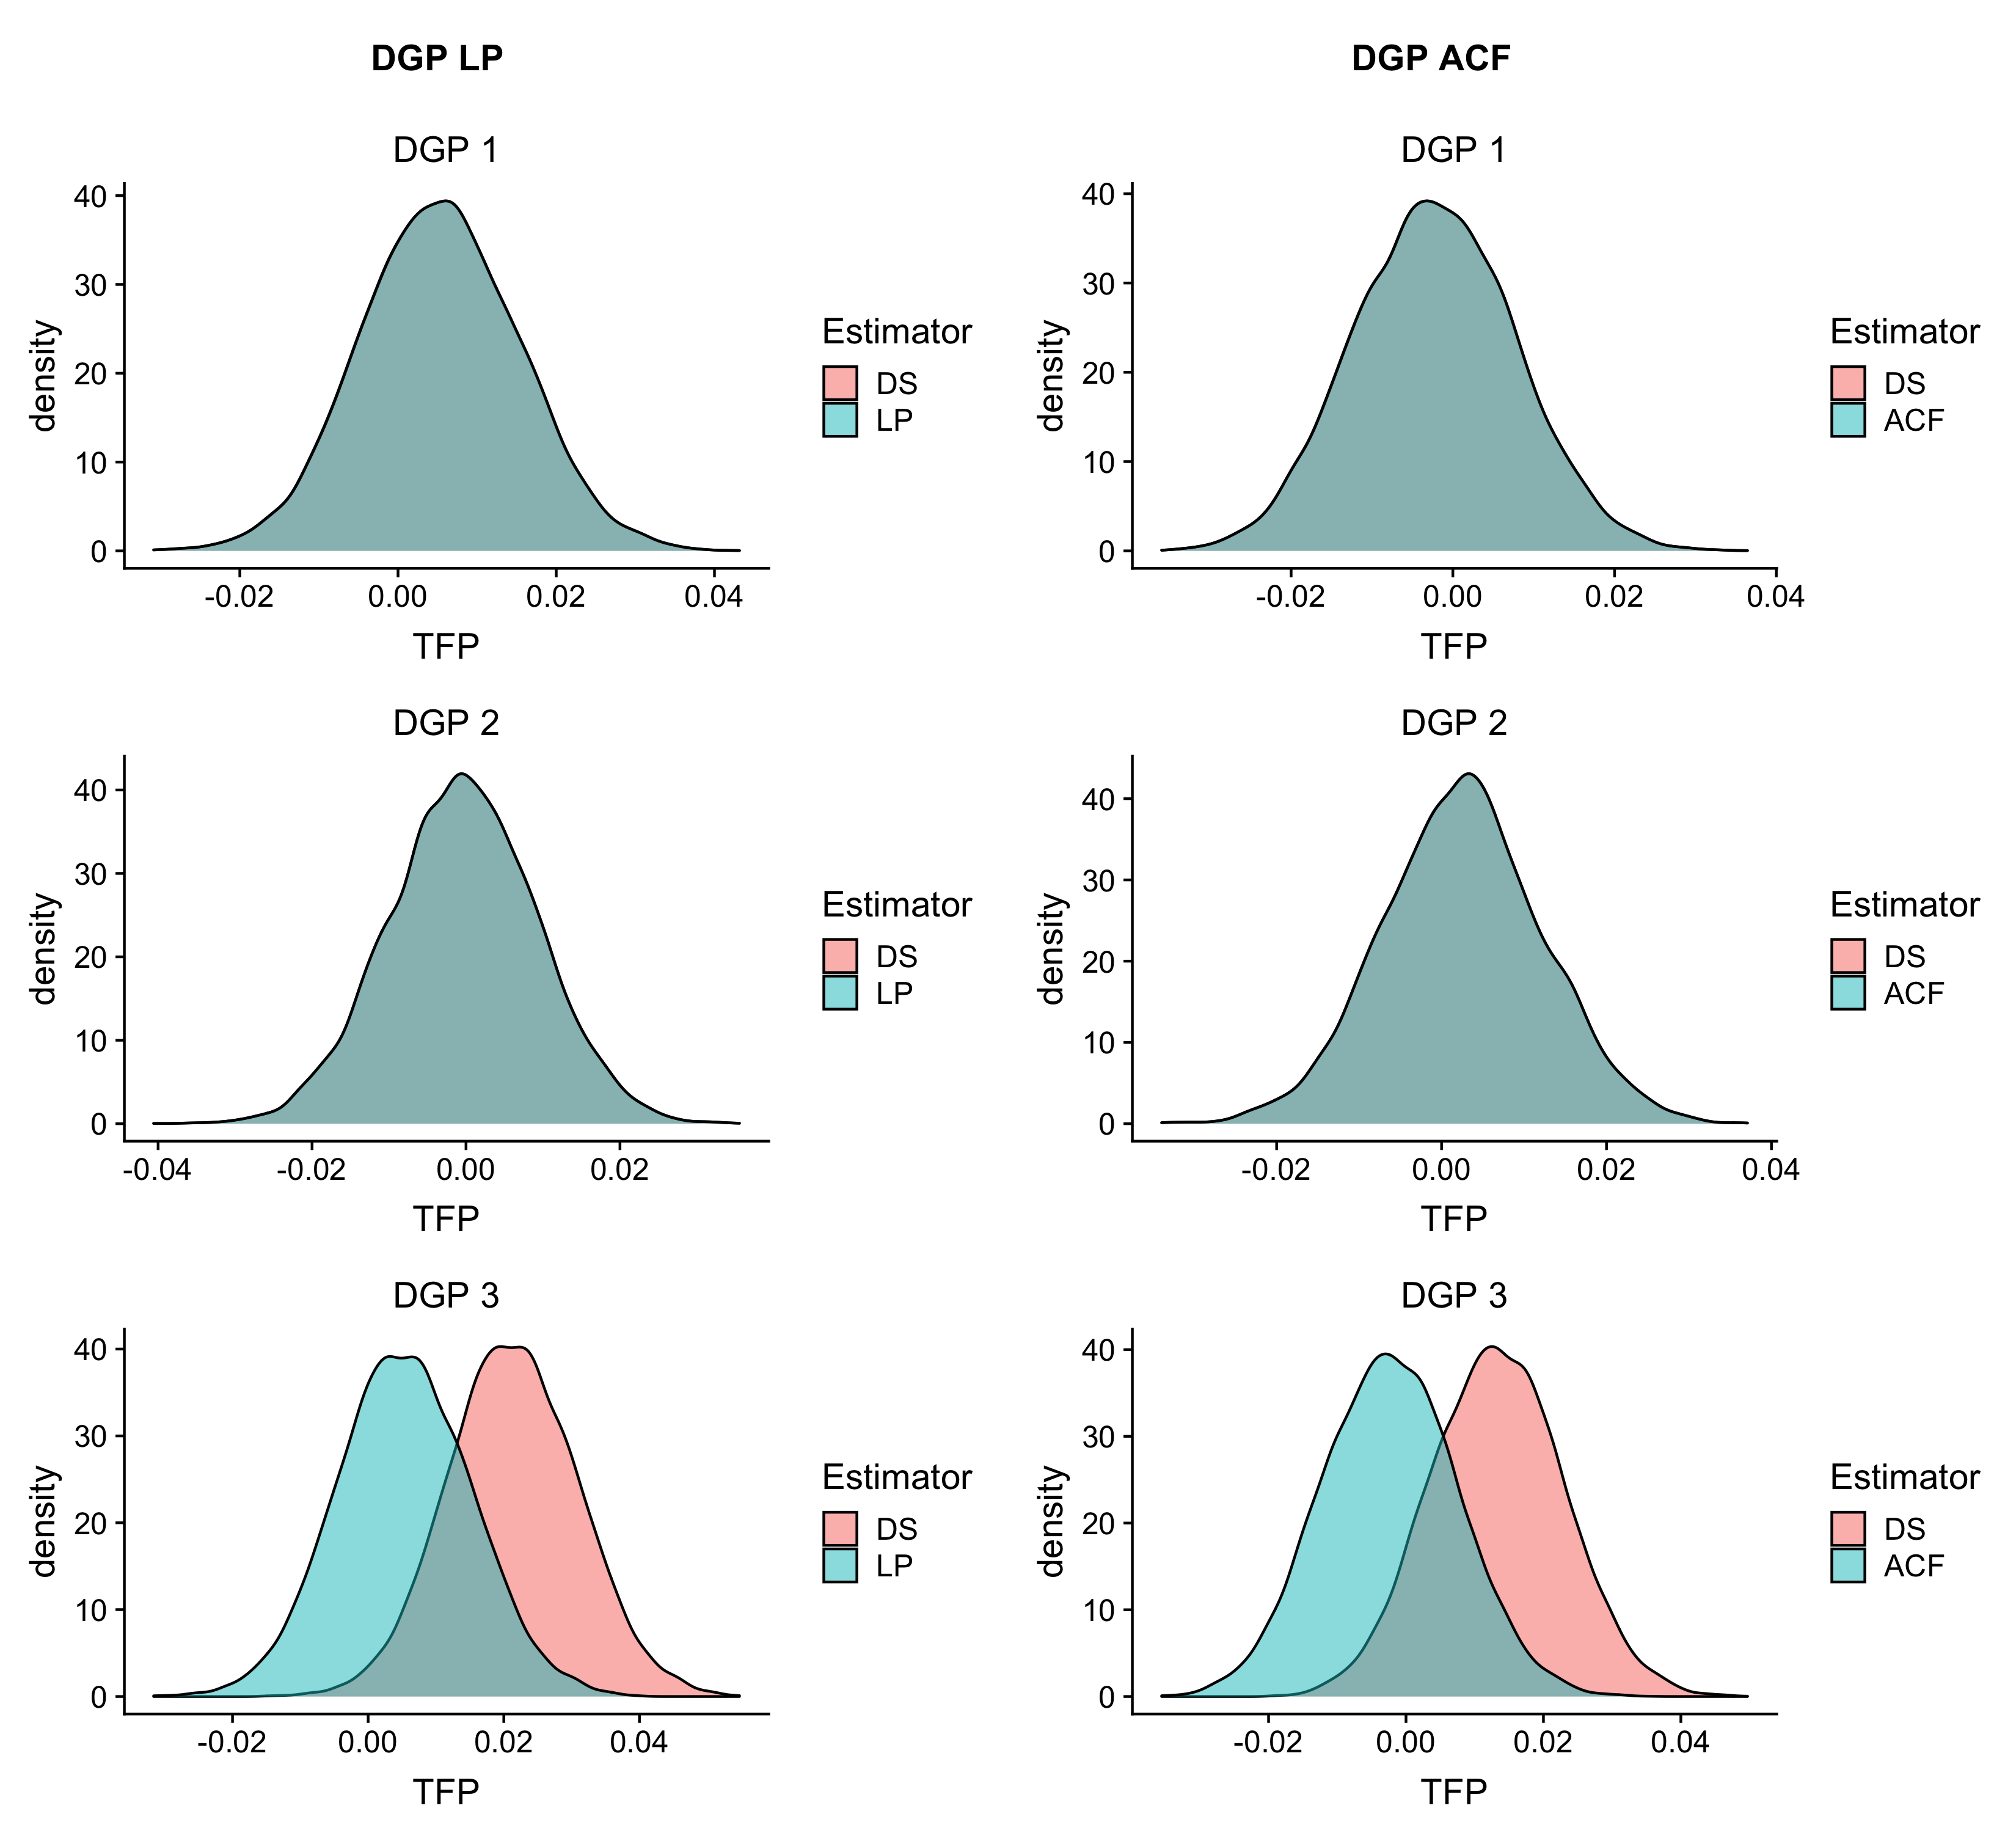
\includegraphics[width=12cm, height=12cm]{MC/TFPplot.png}
\caption*{\footnotesize $^{*}$Estimated TFP from LP, ACF, and the median DS estimator for three DGPs: The left panel compares the LP estimator and the DS estimator when productivity is estimated using LP; The right panel compares the ACF estimator and the DS estimator when productivity is estimated using ACF.}
\label{fig:MCTFP}
\end{figure}

\section{Application} \label{application}
We apply our estimator to firm and plant-level manufacturing datasets from the U.S., Chile, and Colombia to examine heterogeneity in production. For each country, we examine estimates across different manufacturing industries as well as how estimates of productivity have changed over time. We use the DS estimator with productivity estimated using ACF and compare it to the conditional mean estimates from ACF. We also compare our estimates to the quantile regression estimates without controlling for productivity. In Appendix \ref{gross} we estimate a gross-output production function with productivity estimated using LP. In the ACF estimation procedure, we estimate the non-parametric function $\Phi_{t}$ with a 2nd degree polynomial with interactions in capital, labor, and materials. To estimate the coefficients on capital and labor, we use the ACF criterion function mentioned earlier. Since we only need a consistent estimator of the production function parameters, we do not consider any over-identification conditions in this step. We use bootstrap to estimate standard errors of $\beta_{k}(\tau)$ and $\beta_{l}(\tau)$ with the number of iterations set to $500$.
%----------------------------------------------------------------------------------------
\subsection{U.S. Compustat}
The source for the U.S. manufacturing data is from Compustat which covers publicly traded firms and contains data from their financial statements. We collect a sample between 1961 and 2016 on sales, capital expenditures, number of workers, and other expenses which are deflated to construct measures of output, capital, labor, and material inputs. Data preparation follows \cite{Keller2009} and \cite{mert}. Manufacturing industries are classified by the first digit NAICS codes 31-33. NAICS 31 includes different types of food and beverage manufacturing as well as manufacturing of textiles and apparels. NAICS 32 includes manufacturing of wood, paper, chemicals, and plastics. NAICS 33 includes steel, mineral, and equipment, and electronic manufacturing. We also aggregate the three industries to obtain estimates from the entire manufacturing firms. Summary statistics for these deflated values are provided in Appendix \ref{USdata}. We present a series of output elasticity estimates in Table \ref{USQACF} which are illustrated graphically in Figures \ref{fig:QACFUS31}, \ref{fig:QACFUS32}, \ref{fig:QACFUS33}, and \ref{fig:QACFUSall}. 

In each of these figures, we plot estimates for $\tau\in\{0.05, 0.1,\dots, 0.95\}$. In the first row of plots for each figure, the horizontal axis denotes these percentiles and the vertical axis is the estimated output elasticities. The solid black line denotes our estimator under different $\tau$ with its corresponding $90\%$ point-wise confidence interval shaded in dark gray. The solid red line denotes the conditional mean estimates of the output elasticities using ACF and the dotted red lines is the corresponding $90\%$ confidence interval. The bottom row presents the difference between our estimator and the conditional quantile estimator without taking into account the endogeneity of productivity. The horizontal axis denotes the percentiles and the vertical axis denotes the difference between the estimates. The solid black dots are the point estimates of these differences and the solid black line denotes their corresponding $95\%$ confidence intervals. 

Estimates of the capital elasticity are increasing in $\tau$ in every industry as well as the combined sample. The estimates for labor elasticity for each industry and the combined sample are decreasing. In each industry, aside from NAICS 31, there is evidence that our model captures heterogeneity relative to the ACF model. The small number of samples in NAICS 31 contribute to higher estimated standard errors for the output elasticities as well as other estimates such as capital intensity. In each industry, there are large differences between estimates at low and high quantiles. In NAICS 31, the capital estimates range from 0.3 to 0.8 and the labor estimates range from 0.9 to 0.17. For every other industry, the capital estimates range from close to zero to 0.4, whereas the labor estimates range from close to one to about 0.6.

In each industry, we compare the differences between our estimates and QR estimates to test whether our model corrects for endogeneity from unobserved productivity. Bootstrap is used to construct confidence intervals of the difference between the two estimates. We find that most differences occur at the lower tail of the conditional output distribution. We also use the estimates from the output elasticities to construct measures of returns to scale and capital intensity in Table \ref{USQACF}. Each industry has estimates of returns to scale that decreasing in $\tau$ and capital intensity that increase with $\tau$. Table \ref{USACF} shows the results using the ACF estimator. The estimated coefficients are comparable to those at the median ($\tau=0.5$) in Table \ref{USQACF}.

\begin{figure}[H]
\centering
\caption{Estimated Coefficients of Capital and Labor for U.S.: NAICS 31}
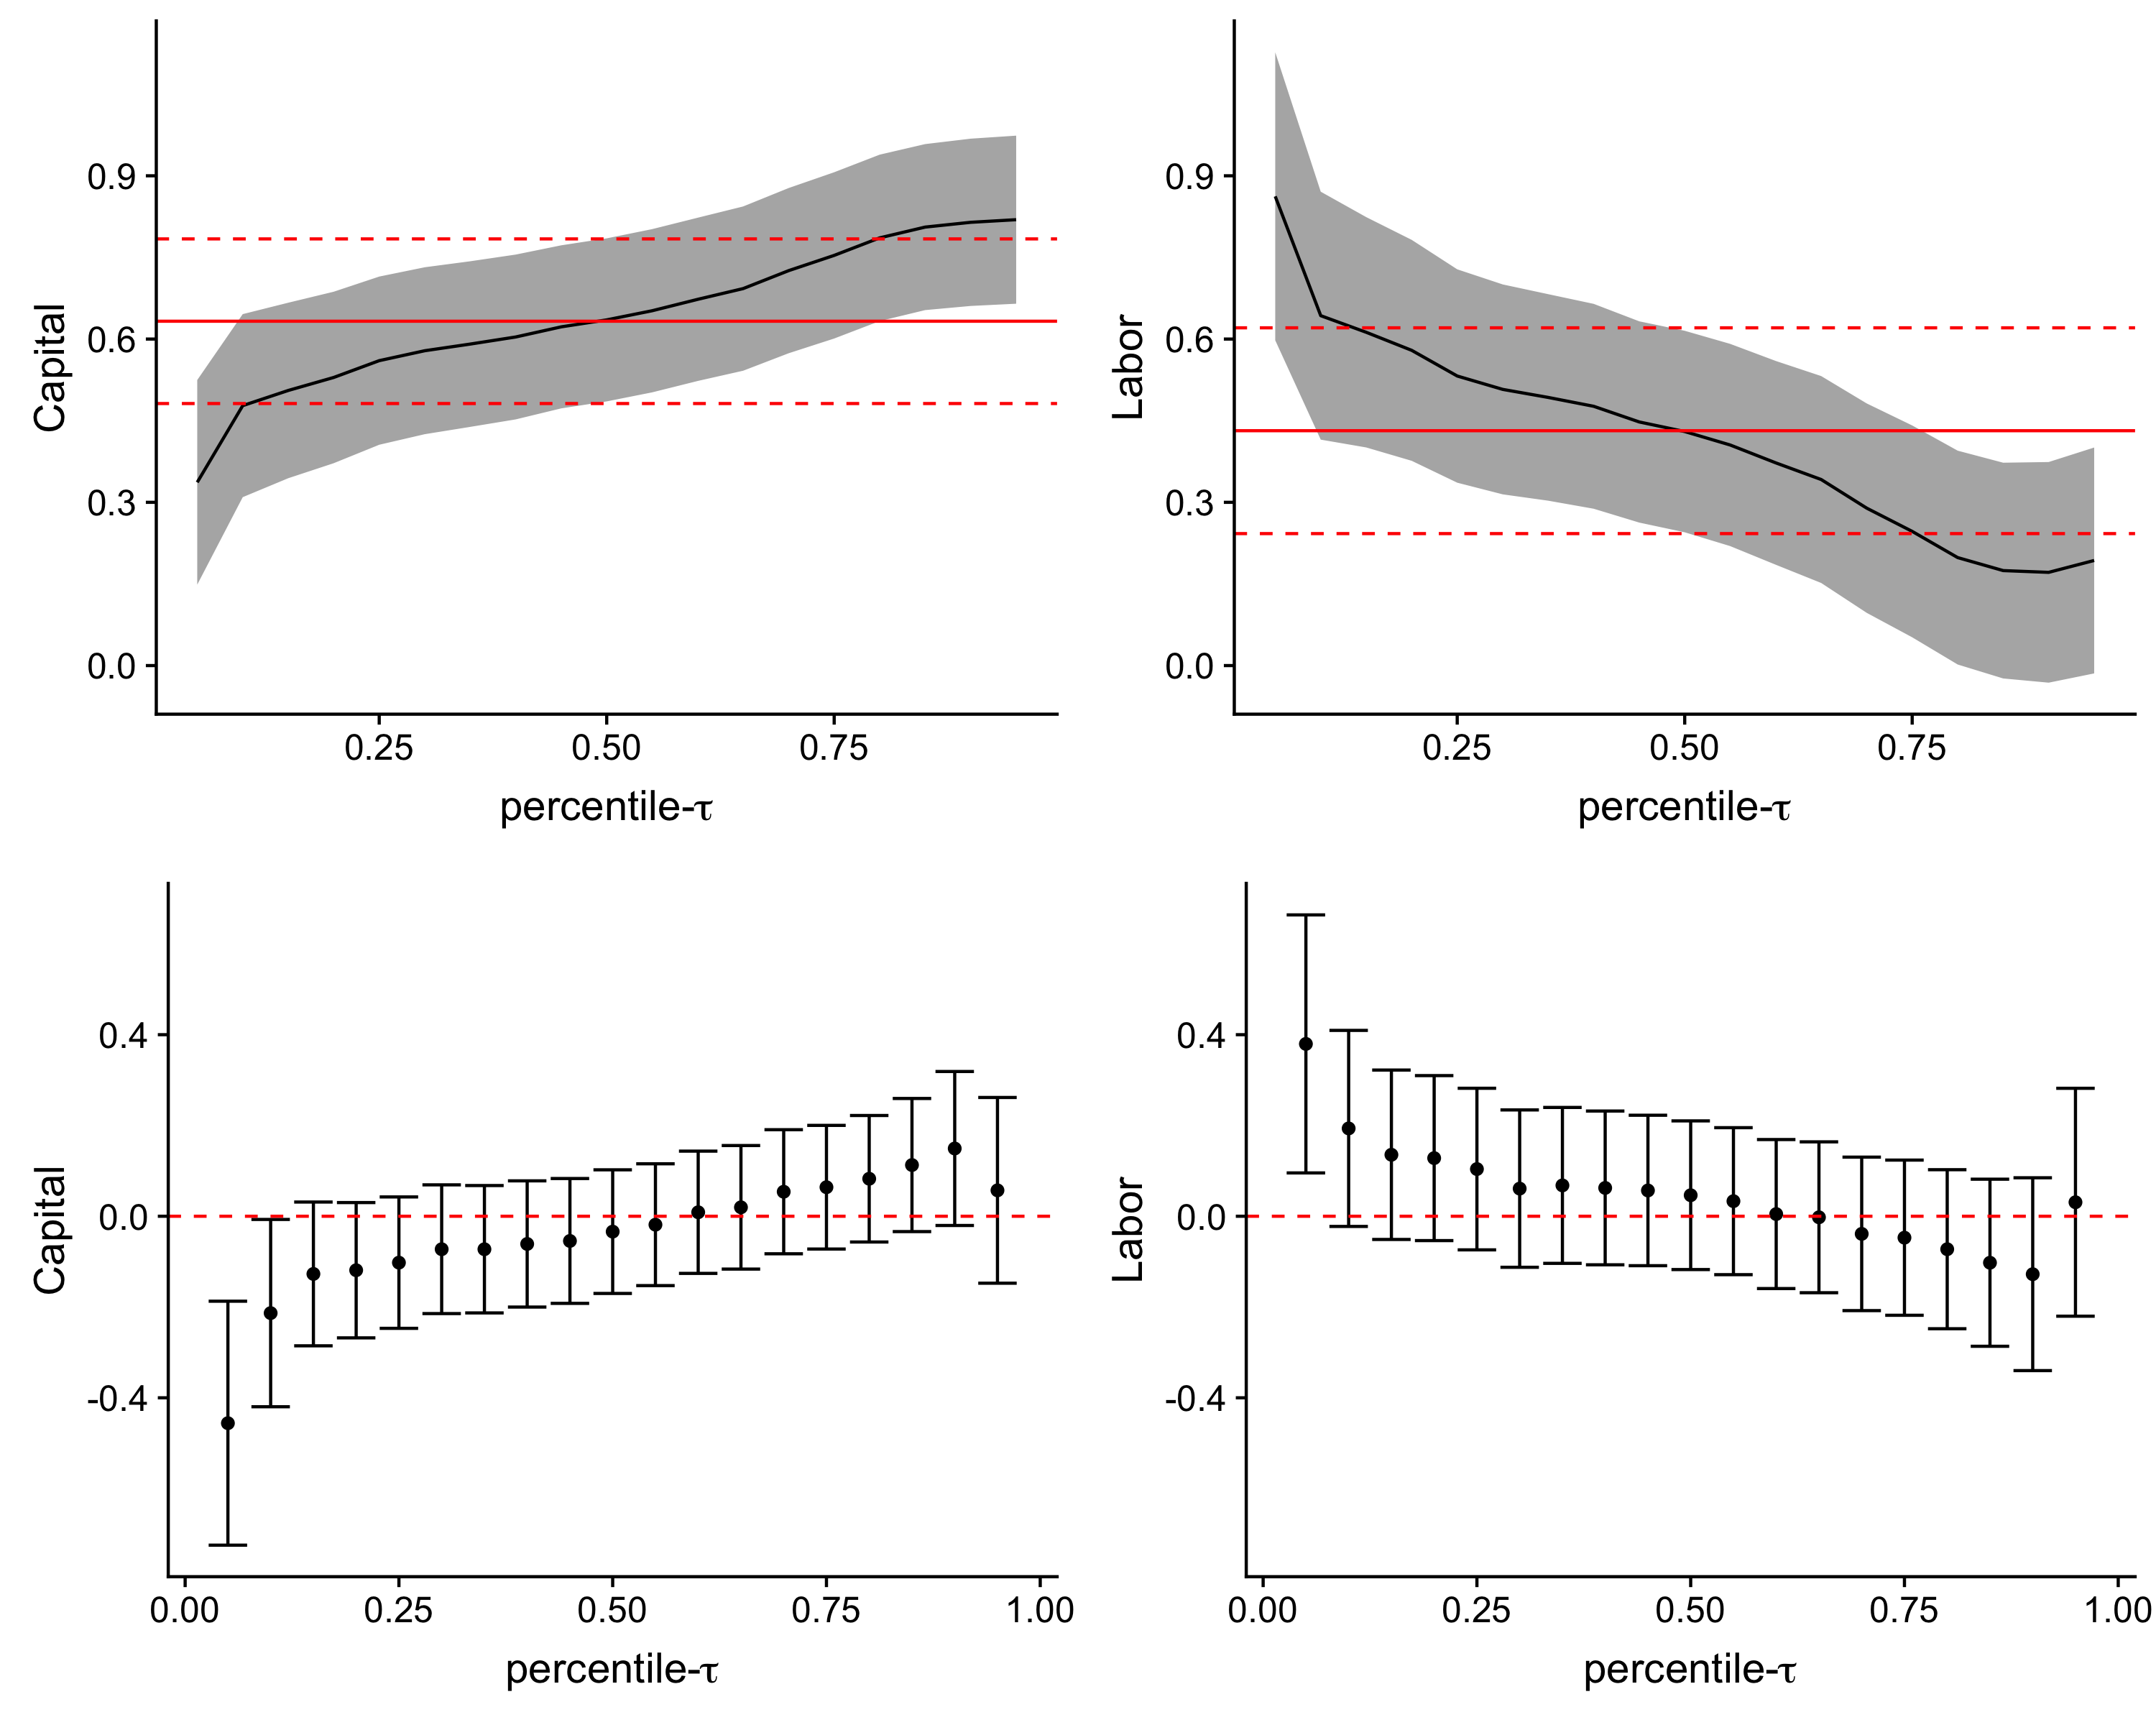
\includegraphics[width=8cm, height=8cm]{US/QACF_Coef_Plot_NAICS_31.png}
\caption*{\footnotesize $^{*}$Top row: Estimated values of production function coefficients and their point-wise 90\% confidence interval. Bottom row: Difference between DS and QR estimates that does not control for endogeneity and their 95\% confidence intervals.}
\label{fig:QACFUS31}
\end{figure}

\begin{figure}[H]
\centering
\caption{Estimated Coefficients of Capital and Labor for U.S.: NAICS 32}
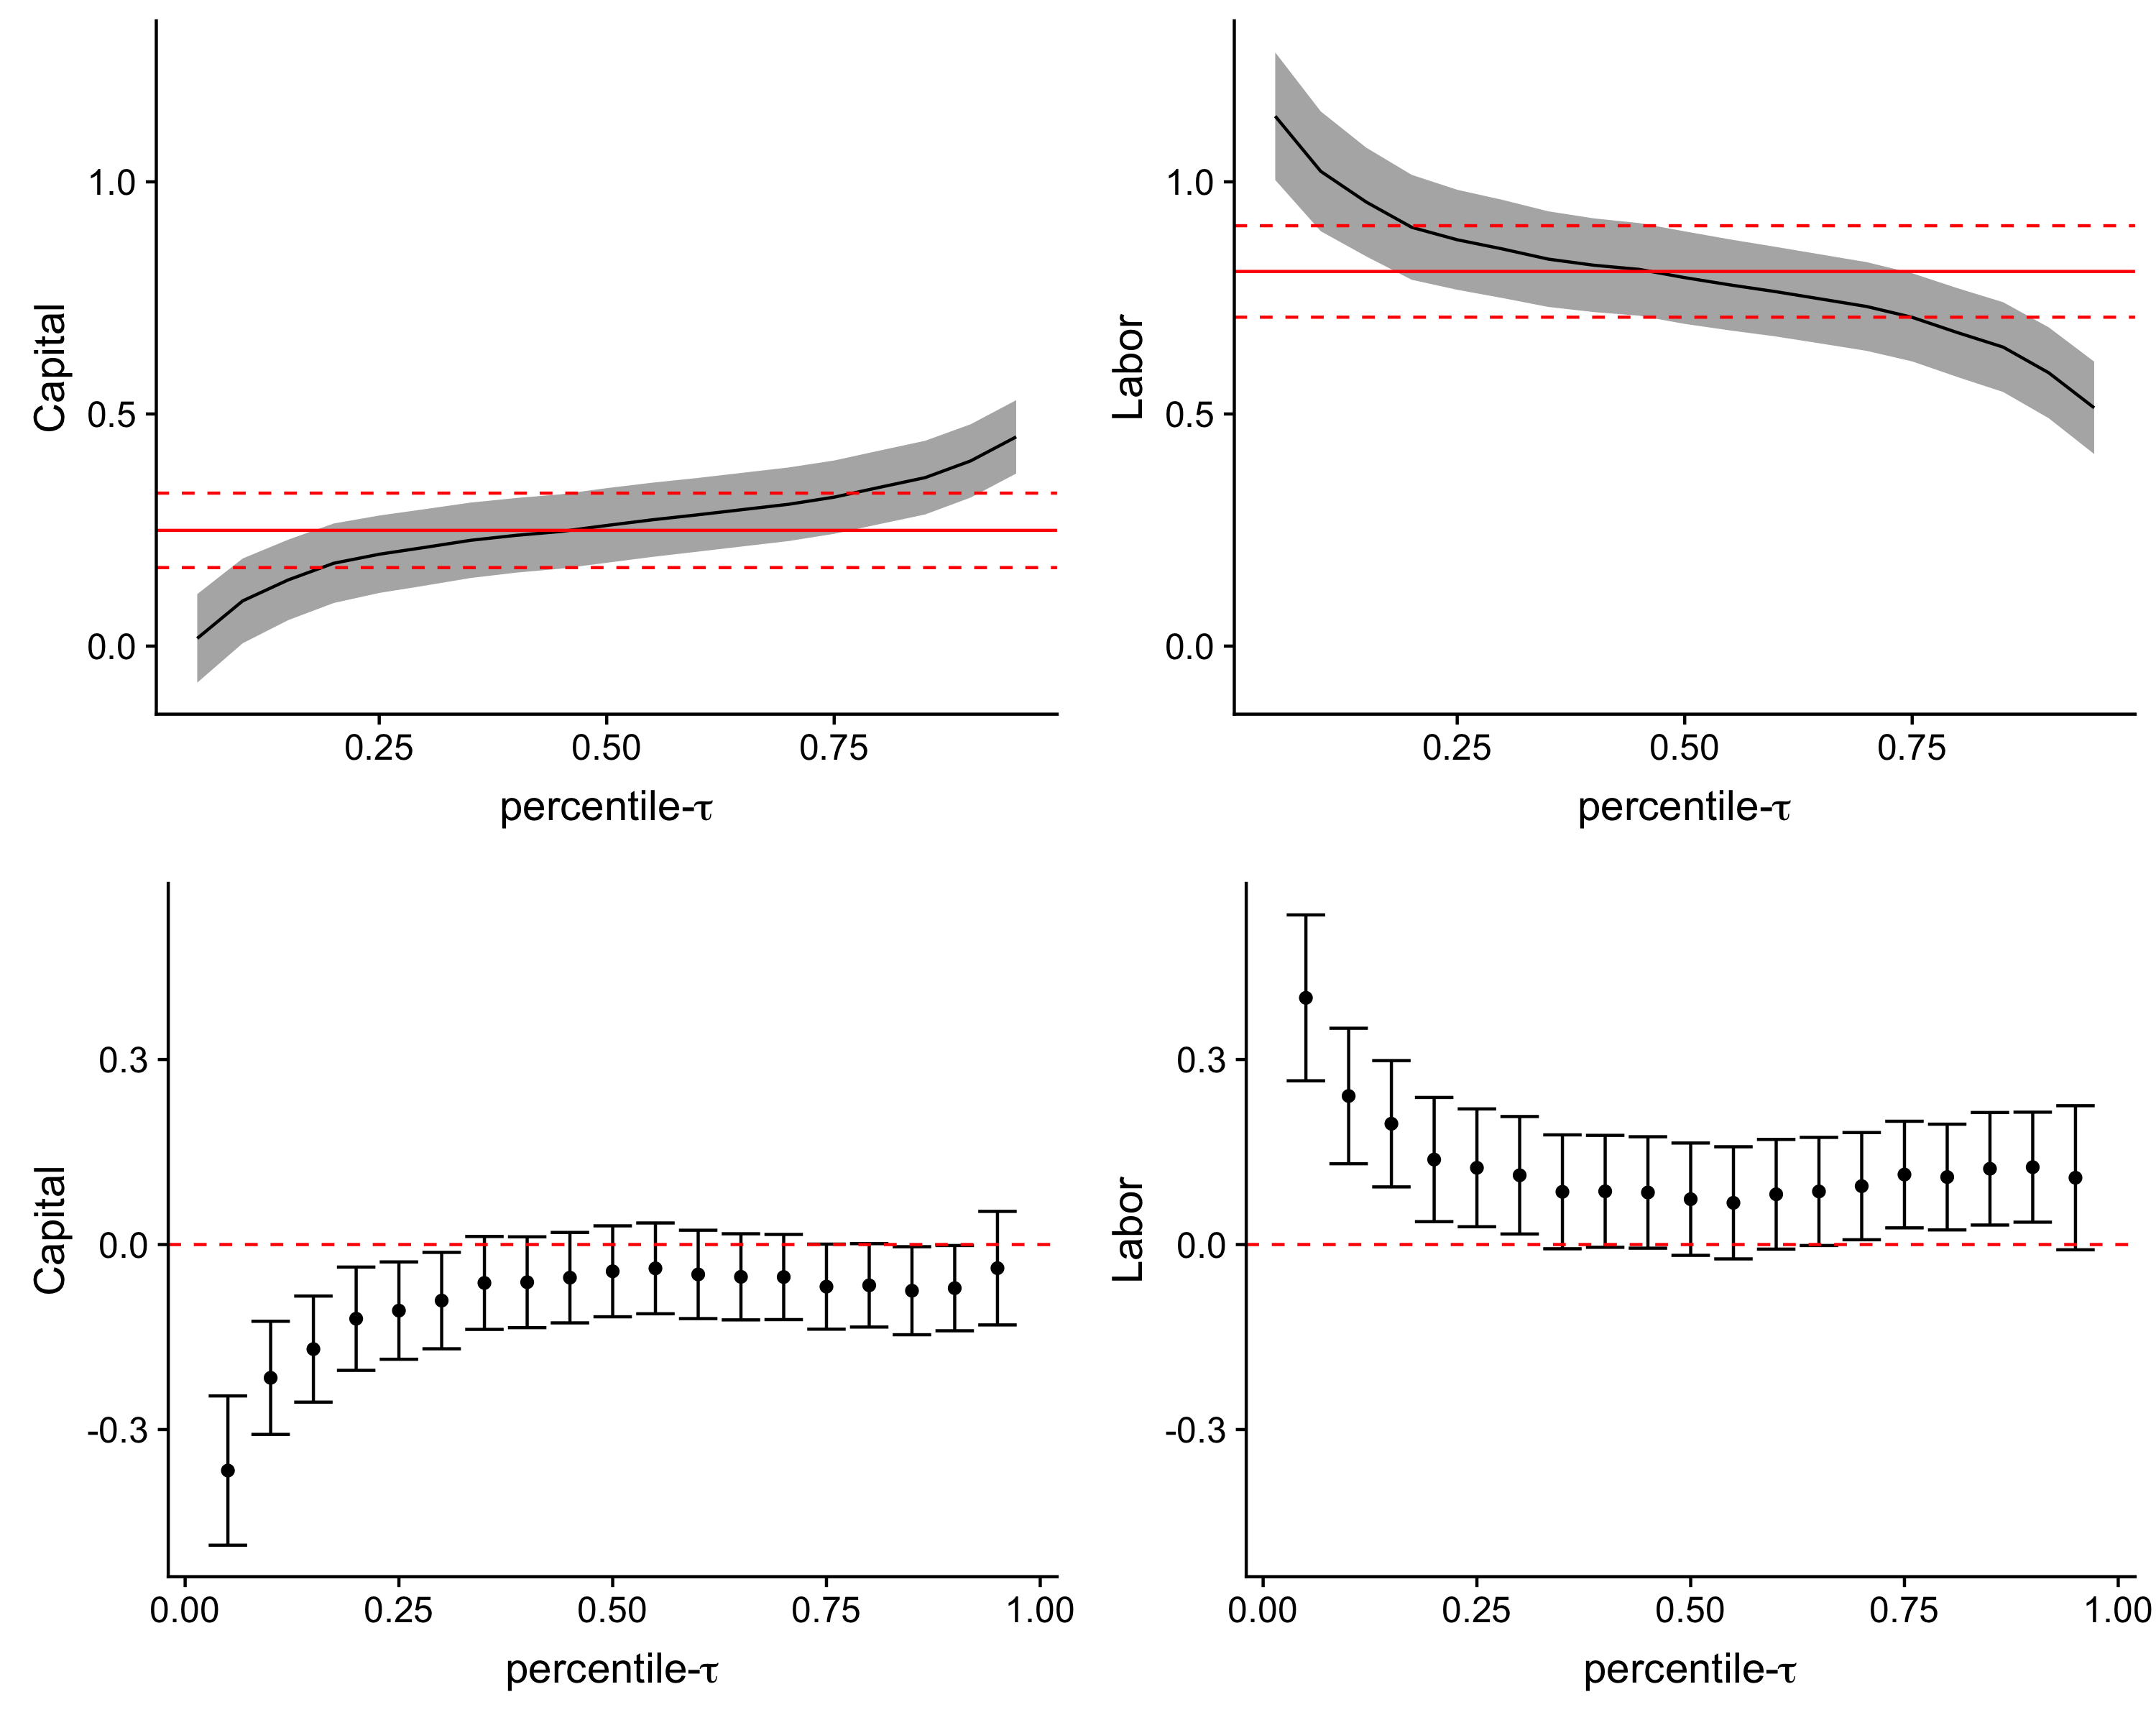
\includegraphics[width=8cm, height=8cm]{US/QACF_Coef_Plot_NAICS_32.png}
\caption*{\footnotesize $^{*}$Top row: Estimated values of production function coefficients and their point-wise 90\% confidence interval. Bottom row: Difference between DS and QR estimates that does not control for endogeneity and their 95\% confidence intervals.}
\label{fig:QACFUS32}
\end{figure}

\begin{figure}[H]
\centering
\caption{Estimated Coefficients of Capital and Labor for U.S.: NAICS 33}
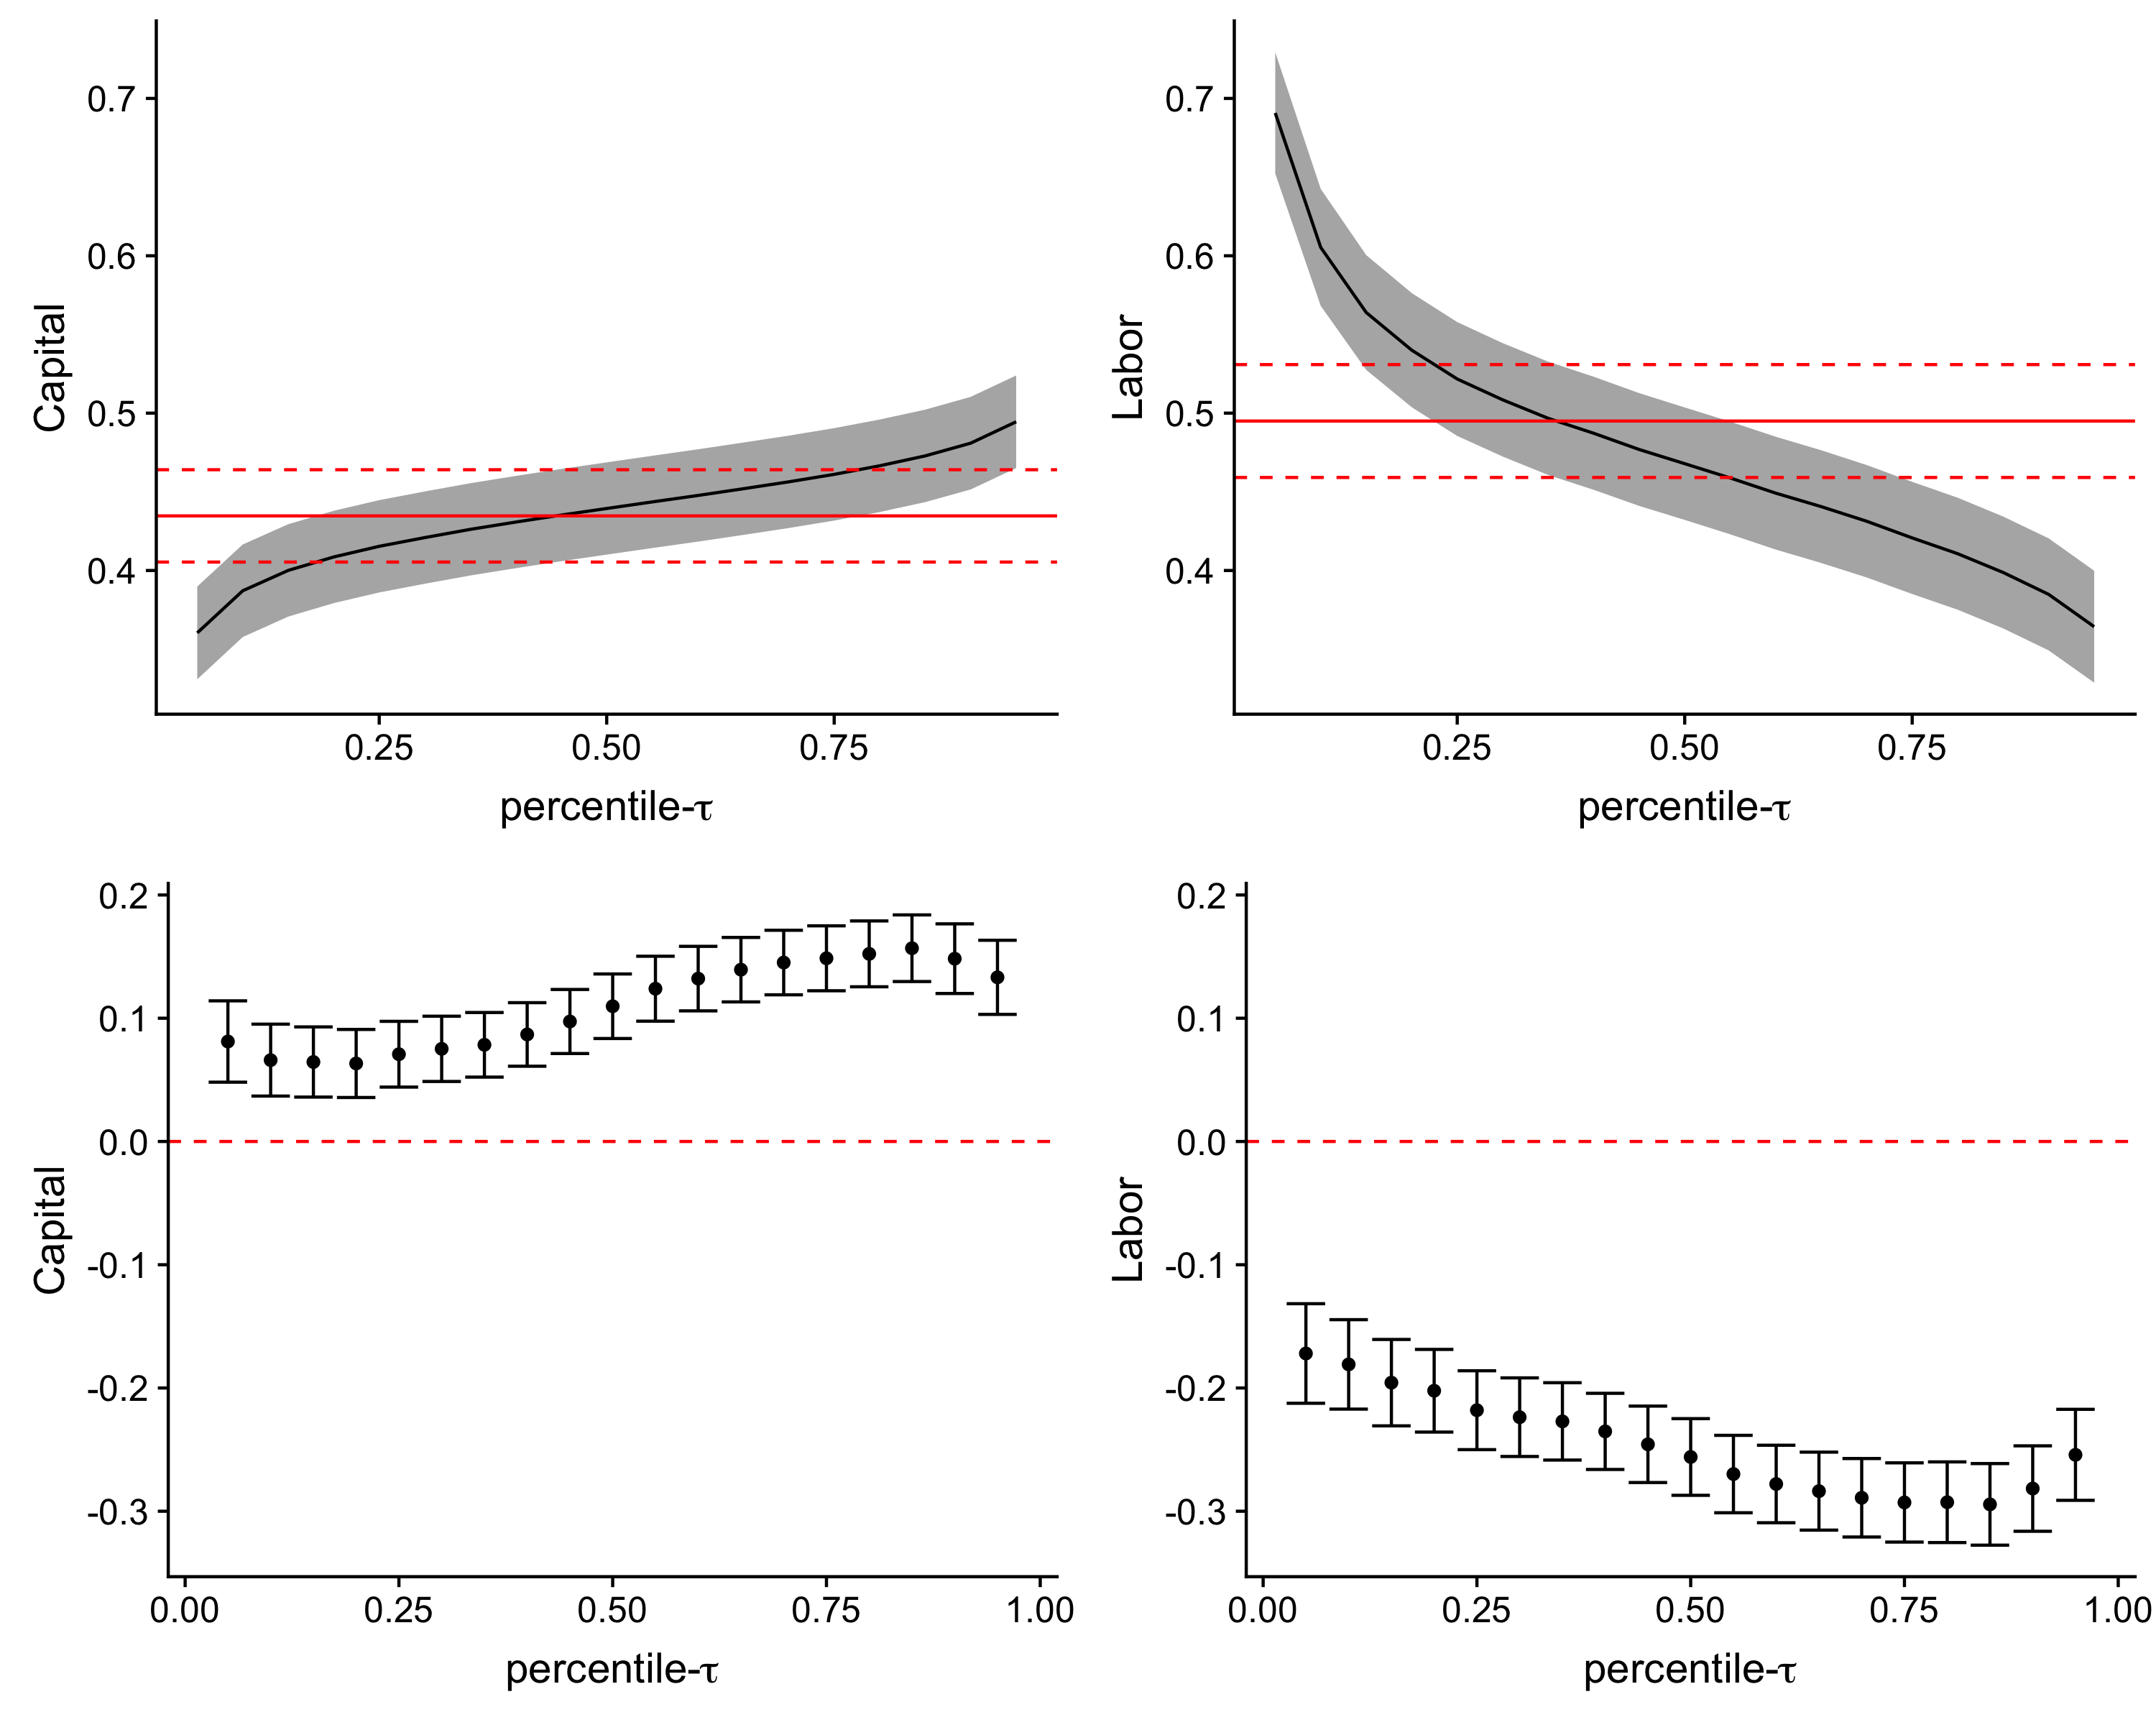
\includegraphics[width=8cm, height=8cm]{US/QACF_Coef_Plot_NAICS_33.png}
\caption*{\footnotesize $^{*}$Top row: Estimated values of production function coefficients and their point-wise 90\% confidence interval. Bottom row: Difference between DS and QR estimates that does not control for endogeneity and their 95\% confidence intervals.}
\label{fig:QACFUS33}
\end{figure}

\begin{figure}[H]
\centering
\caption{Estimated Coefficients of Capital and Labor for U.S. Manufacturing Firms}
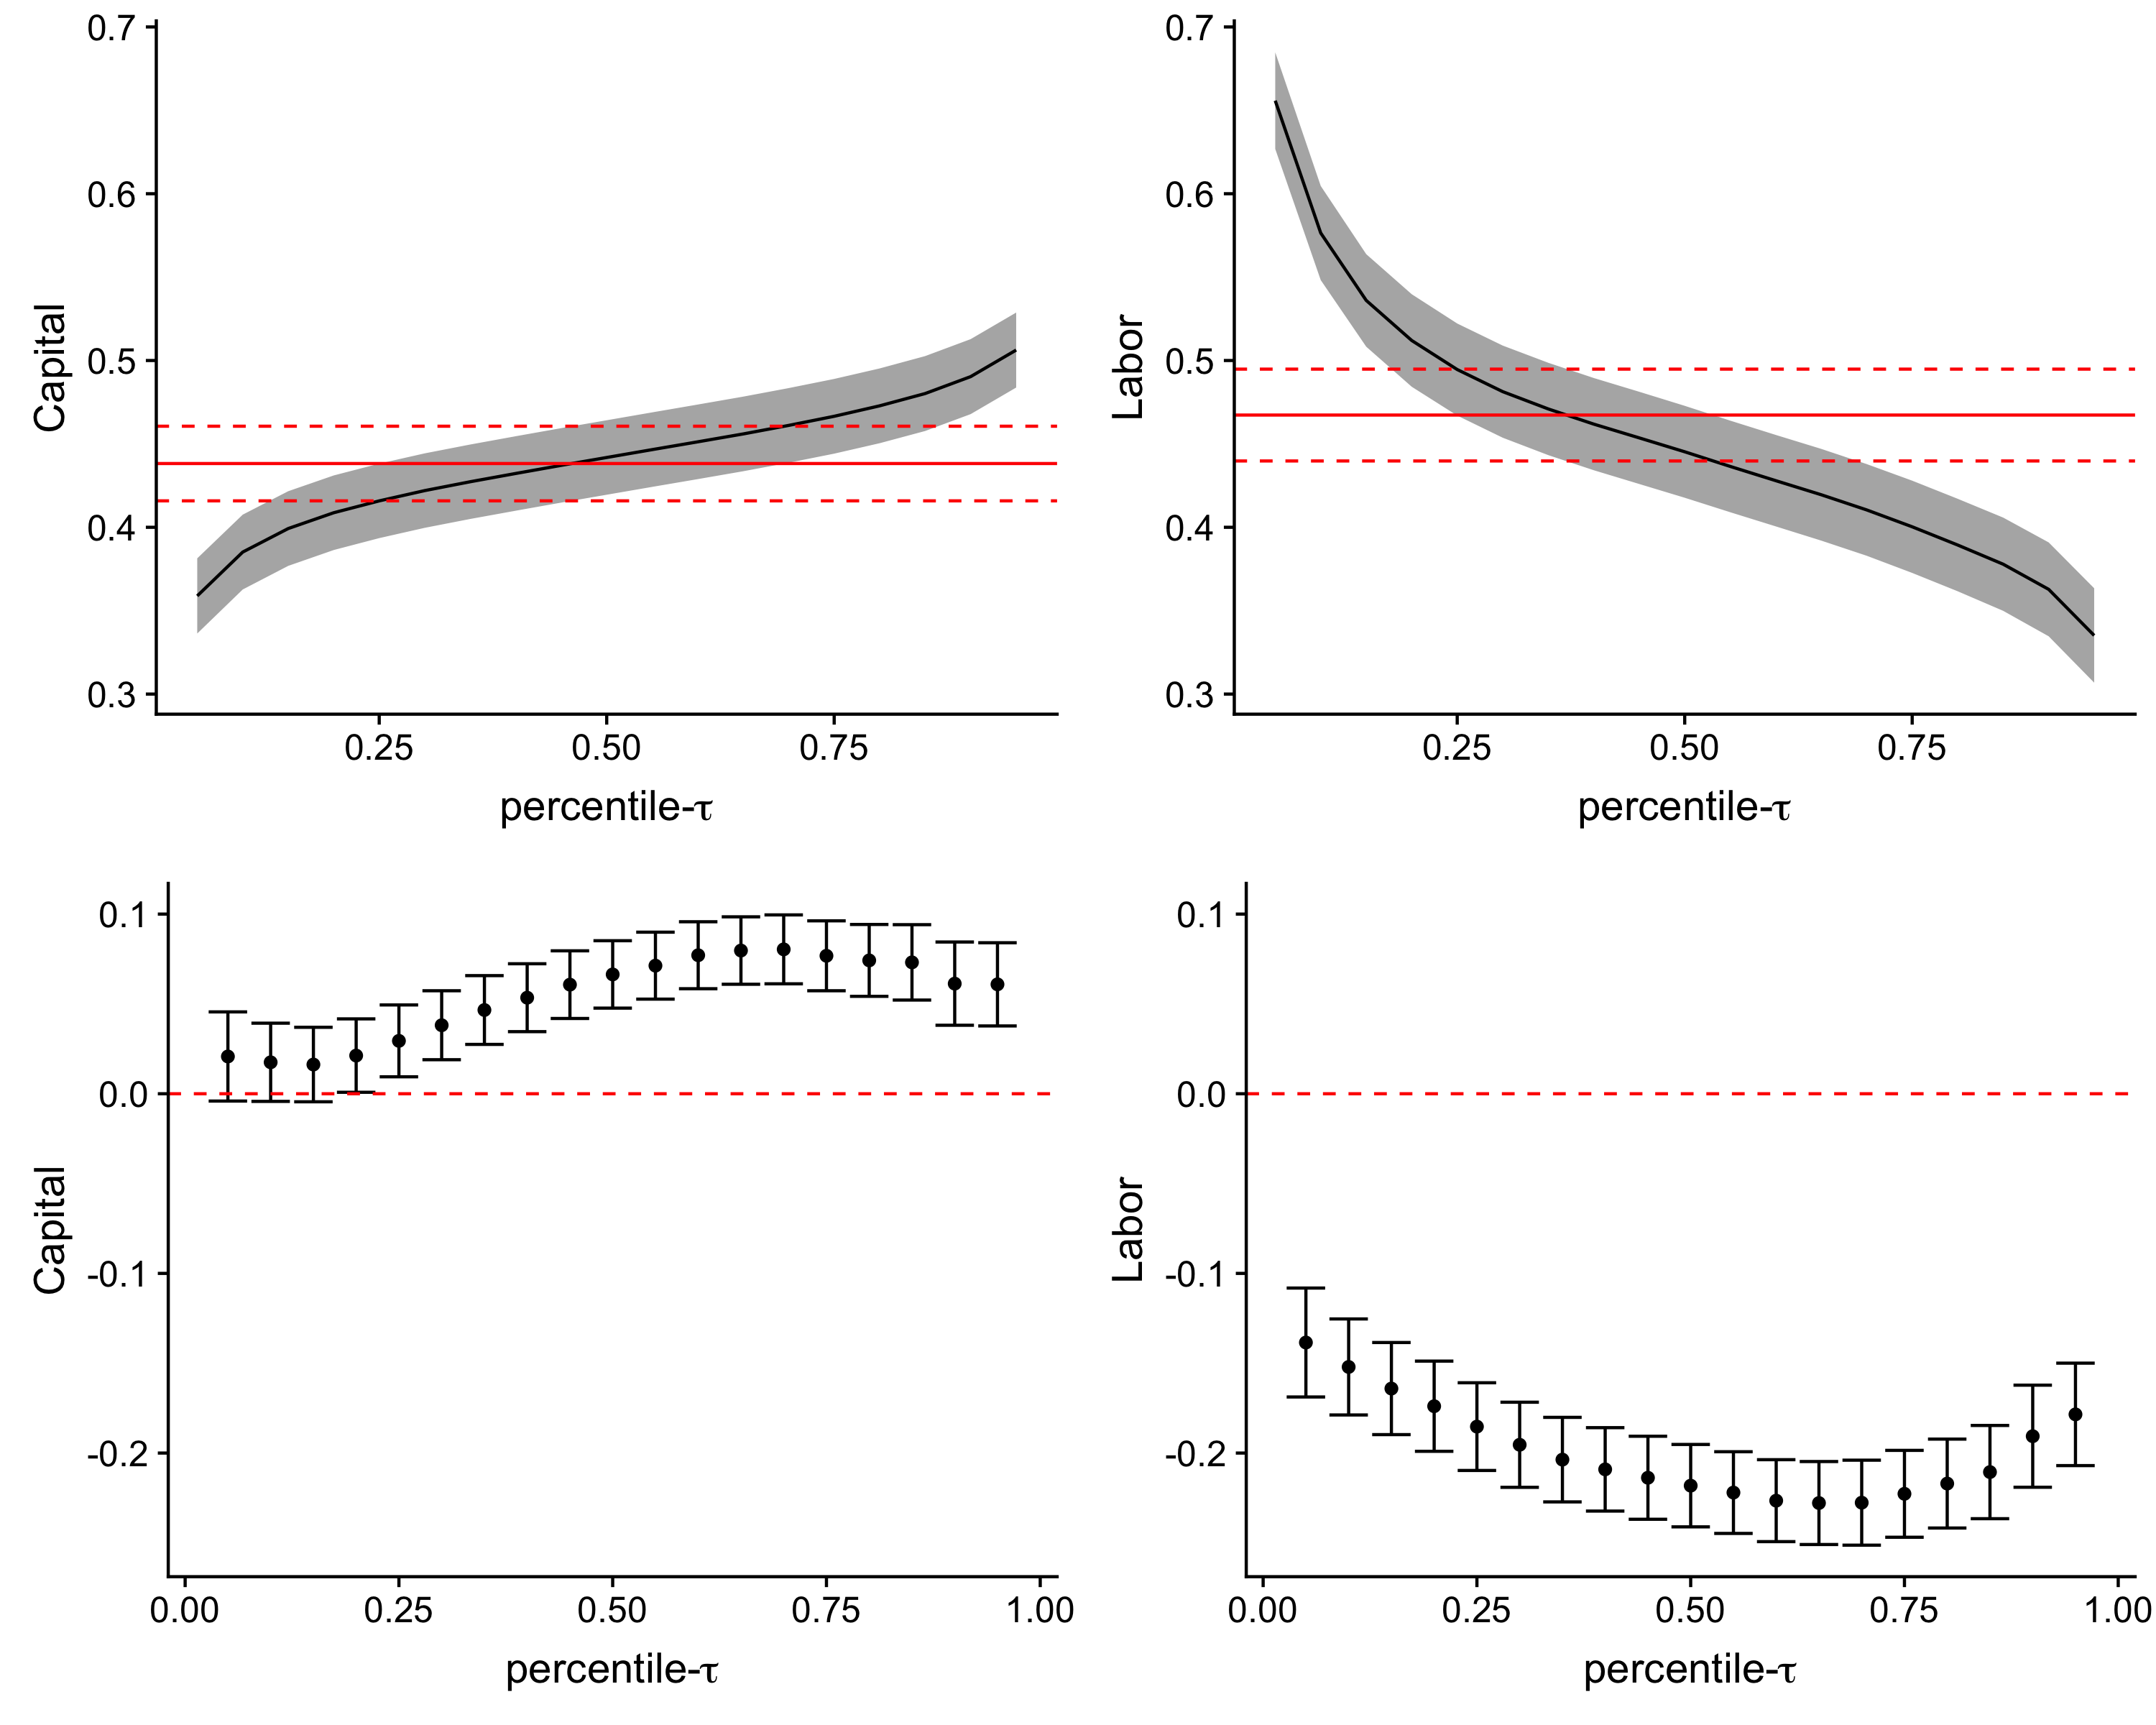
\includegraphics[width=8cm, height=8cm]{US/QACF_Coef_Plot_NAICS_All.png}
\caption*{\footnotesize $^{*}$Top row: Estimated values of production function coefficients and their point-wise 90\% confidence interval. Bottom row: Difference between DS and QR estimates that does not control for endogeneity and their 95\% confidence intervals.}
\label{fig:QACFUSall}
\end{figure}

\begin{table}[H]
\centering
\caption{Coefficient Estimates and Standard Errors for U.S. Manufacturing Firms}
\small
\begin{tabular}{cccccccccc}
  \hline\hline & & \multicolumn{2}{c}{Capital}  & \multicolumn{2}{c}{Labor} & \multicolumn{2}{c}{Returns to Scale} & \multicolumn{2}{c}{Capital Intensity}\\ \cmidrule(lr){3-4} \cmidrule(lr){5-6} \cmidrule(lr){7-8} \cmidrule(lr){9-10}NAICS & $\tau$ & Coef. & s.e & Coef. & s.e & Coef. & s.e & Coef. & s.e \\ 
  \hline
31 & 0.10 & 0.319 & 0.0323 & 0.554 & 0.0383 & 0.873 & 0.0161 & 0.575 & 0.0787 \\ 
   & 0.25 & 0.345 & 0.0324 & 0.500 & 0.0375 & 0.845 & 0.0143 & 0.689 & 0.0915 \\ 
   & 0.50 & 0.372 & 0.0323 & 0.450 & 0.0369 & 0.821 & 0.0133 & 0.827 & 0.1073 \\ 
   & 0.90 & 0.422 & 0.0327 & 0.374 & 0.0390 & 0.797 & 0.0204 & 1.127 & 0.1420 \\ 
  32 & 0.10 & 0.189 & 0.0280 & 0.766 & 0.0359 & 0.955 & 0.0132 & 0.246 & 0.0478 \\ 
   & 0.25 & 0.217 & 0.0279 & 0.692 & 0.0349 & 0.909 & 0.0119 & 0.313 & 0.0555 \\ 
   & 0.50 & 0.242 & 0.0279 & 0.639 & 0.0346 & 0.881 & 0.0114 & 0.378 & 0.0630 \\ 
   & 0.90 & 0.293 & 0.0278 & 0.540 & 0.0354 & 0.833 & 0.0127 & 0.543 & 0.0835 \\ 
  33 & 0.10 & 0.387 & 0.0179 & 0.605 & 0.0226 & 0.992 & 0.0070 & 0.640 & 0.0283 \\ 
   & 0.25 & 0.415 & 0.0178 & 0.522 & 0.0220 & 0.937 & 0.0061 & 0.796 & 0.0330 \\ 
   & 0.50 & 0.439 & 0.0178 & 0.468 & 0.0217 & 0.907 & 0.0058 & 0.939 & 0.0371 \\ 
   & 0.90 & 0.481 & 0.0179 & 0.385 & 0.0216 & 0.866 & 0.0057 & 1.250 & 0.0459 \\ 
  All & 0.10 & 0.385 & 0.0136 & 0.576 & 0.0172 & 0.962 & 0.0055 & 0.668 & 0.0262 \\ 
   & 0.25 & 0.416 & 0.0136 & 0.495 & 0.0168 & 0.910 & 0.0049 & 0.841 & 0.0311 \\ 
   & 0.50 & 0.442 & 0.0136 & 0.445 & 0.0168 & 0.887 & 0.0052 & 0.992 & 0.0354 \\ 
   & 0.90 & 0.490 & 0.0137 & 0.363 & 0.0171 & 0.853 & 0.0064 & 1.352 & 0.0458 \\ 
   \hline
\end{tabular}
\caption*{\footnotesize $^{*}$Standard errors are obtained using bootstrap with 500 replications. The first stage uses estimates from ACF.}
\label{USQACF}
\end{table}

\begin{table}[H]
\centering
\caption{ACF Coefficient Estimates and Standard Errors for U.S. Manufacturing Firms}
\small
\begin{tabular}{ccccccccc}
  \hline\hline & \multicolumn{2}{c}{Capital} & \multicolumn{2}{c}{Labor} & \multicolumn{2}{c}{Returns to Scale} & \multicolumn{2}{c}{Capital Intensity}\\ \cmidrule(lr){2-3} \cmidrule(lr){4-5} \cmidrule(lr){6-7} \cmidrule(lr){8-9}NAICS & Coef. & s.e & Coef. & s.e & Coef. & s.e & Coef. & s.e \\ 
  \hline
31 & 0.370 & 0.0324 & 0.463 & 0.0366 & 0.833 & 0.0130 & 0.800 & 0.1027 \\ 
  32 & 0.240 & 0.0279 & 0.654 & 0.0347 & 0.894 & 0.0108 & 0.367 & 0.0612 \\ 
  33 & 0.435 & 0.0178 & 0.495 & 0.0218 & 0.930 & 0.0057 & 0.878 & 0.0352 \\ 
  All & 0.438 & 0.0136 & 0.467 & 0.0167 & 0.906 & 0.0050 & 0.938 & 0.0337 \\ 
   \hline
\end{tabular}
\caption*{\footnotesize $^{*}$Standard errors are obtained using bootstrap with 500 replications.}
\label{USACF}
\end{table}

We also use our quantile production function estimates to construct measures of firm level productivity which we define as
\begin{equation}
\widehat{TFP}_{it,\tau}=\exp(y_{it}-\hat{\beta}_{k}(\tau)k_{it}-\hat{\beta}_{l}(\tau)l_{it}).
\end{equation}
We use these measures to compare the distributions of productivity and productivity growth over time to ACF estimates over the conditional output distribution. Figure \ref{fig:QACFUSTFP} plots densities of TFP for $\tau \in \{0.1, 0.5, 0.9\}$ and for the ACF estimator. The plot shows apparent differences between TFP estimates for low and high $\tau$, but not much difference between $\tau=0.5$ and the mean estimates of ACF. Figure \ref{fig:QACFUSTFPG} reports average productivity for each industry with the base year of the sample period set to 100. We can see that productivity growth was steady in the beginning of the sample period but then declined after the year 2000 followed by a period of high productivity growth. Growth trends for each percentile were similar although firms who rank lower on the conditional output distribution in this sample were more productive than higher ranked firms. Lower ranked firms may have higher managerial efficiency and can adapt to market changes faster than higher ranked firms. The ACF estimates are close to the productivity estimates for firms at $\tau=0.5$. The figure also shows that productivity dispersion across $\tau$ has been gradually increasing over time which is consistent which is consistent with the existing empirical literature which find increasing productivity dispersion.
\begin{figure}[H]
\centering
\caption{DS and ACF Estimates of Log Total Factor Productivity}
\includegraphics[width=11cm]{US/QACF_TFP_Plot.png}
\caption*{\footnotesize $^{*}$Estimated Distributions of TFP from the DS estimator for $\tau \in \{0.1, 0.5, 0.9\}$ and those from  the ACF estimator.}
\label{fig:QACFUSTFP}
\end{figure}

\begin{figure}[H]
\centering
\caption{U.S. Productivity Over Time}
\includegraphics[width=11cm]{US/QACF_TFPgrowth_Plot.png}
\caption*{\footnotesize $^{*}$Estimated average productivity (in levels) over time for the U.S. Base year productivity is set to 100.}
\label{fig:QACFUSTFPG}
\end{figure}

In Table \ref{QACFUSTFPP} we examine the effect of R\&D and advertising intensity on productivity across the conditional output distribution. Specifically, we regress the estimated productivity on R\&D and advertising intensity for each $\tau$, where all variables are log-transformed. Our results show that as $\tau$ increases, the returns to R\&D and advertising also increase. Comparing the median estimates to the ACF estimates in Table \ref{ACFUSTFPP}, we observe that in NAICS 33, the return to R\&D for the median firm is $2.5\%$ and the return to advertising is $3\%$, whereas the returns for the average firm are $1\%$ and $1.9\%$, respectively. These results suggest that higher ranked firms are better at converting R\&D and advertising activities into larger productivity gains. 

\begin{table}[H]
\centering
\caption{Productivity Differentials for U.S. Manufacturing Firms using DS}
\small
\begin{tabular}{cccccc}
  \hline\hline & & \multicolumn{2}{c}{R\&D}  & \multicolumn{2}{c}{Advertisements} \\ \cmidrule(lr){3-4} \cmidrule(lr){5-6}NAICS & $\tau$ & Coef. & s.e & Coef. & s.e \\ 
  \hline
31 & 0.10 & 0.157 & 0.0160 & 0.187 & 0.0197 \\ 
   & 0.25 & 0.170 & 0.0143 & 0.200 & 0.0178 \\ 
   & 0.50 & 0.181 & 0.0133 & 0.211 & 0.0162 \\ 
   & 0.90 & 0.190 & 0.0139 & 0.219 & 0.0159 \\ 
  32 & 0.10 & 0.105 & 0.0092 & 0.112 & 0.0105 \\ 
   & 0.25 & 0.133 & 0.0093 & 0.139 & 0.0103 \\ 
   & 0.50 & 0.148 & 0.0088 & 0.154 & 0.0098 \\ 
   & 0.90 & 0.175 & 0.0088 & 0.180 & 0.0099 \\ 
  33 & 0.10 & 0.064 & 0.0054 & 0.048 & 0.0054 \\ 
   & 0.25 & 0.098 & 0.0047 & 0.076 & 0.0047 \\ 
   & 0.50 & 0.115 & 0.0046 & 0.091 & 0.0045 \\ 
   & 0.90 & 0.138 & 0.0050 & 0.109 & 0.0047 \\ 
  All & 0.10 & 0.097 & 0.0047 & 0.082 & 0.0051 \\ 
   & 0.25 & 0.126 & 0.0042 & 0.109 & 0.0045 \\ 
   & 0.50 & 0.138 & 0.0040 & 0.120 & 0.0043 \\ 
   & 0.90 & 0.154 & 0.0042 & 0.133 & 0.0042 \\ 
   \hline
\end{tabular}
\caption*{\footnotesize $^{*}$Standard errors are obtained using bootstrap with 500 replications. Log(TFP) is regressed on log(R\&D) and log(Advertisements).}
\label{QACFUSTFPP}
\end{table}

\begin{table}[H]
\centering
\caption{Productivity Differentials for U.S. Manufacturing Firms using ACF}
\small
\begin{tabular}{ccccc}
  \hline\hline & \multicolumn{2}{c}{R\&D}  & \multicolumn{2}{c}{Advertisements} \\ \cmidrule(lr){2-3} \cmidrule(lr){4-5}NAICS & Coef. & s.e & Coef. & s.e \\ 
  \hline
31 & 0.174 & 0.0132 & 0.204 & 0.0161 \\ 
  32 & 0.140 & 0.0080 & 0.146 & 0.0091 \\ 
  33 & 0.100 & 0.0045 & 0.078 & 0.0046 \\ 
  All & 0.126 & 0.0040 & 0.109 & 0.0043 \\ 
   \hline
\end{tabular}
\caption*{\footnotesize $^{*}$Standard errors are obtained using bootstrap with 500 replications. Log(TFP) is regressed on log(R\&D) and log(Advertisements).}
\label{ACFUSTFPP}
\end{table}

\subsection{Chilean Manufacturing}
This data comes from the census of Chilean manufacturing plants conducted by the Instituto Nacional de Estadist\'ica (INE). The sample is collected between 1979 and 1996 for firms with more than 10 employees. We divide our estimates into the three largest manufacturing industries: Food (ISIC 311), Fabricated Metals (ISIC 381), and Textiles (ISIC 321). We also aggregate the three industries with the other smaller industries to obtain estimates from the entire sample. Summary statistics for the data we use are provided in Table \ref{CHLsum} in Appendix \ref{CHLdata}.

Figures \ref{fig:QACFCHL311}, \ref{fig:QACFCHL381}, \ref{fig:QACFCHL321}, and  \ref{fig:QACFCHLall} illustrate the estimates from our model compared to ACF estimates (top row) as well as the differences between our model and QR estimates that does not control for endogeneity (bottom row). In each industry and the combined sample, estimates of capital elasticity are increasing in $\tau$. In ISIC 321 and the combined sample, these differences are most pronounced in the tails of the conditional output distribution. There is less heterogeneity in the estimates of labor elasticity. In ISIC 311, the estimates of labor elasticity are increasing in $\tau$, but not much different from the mean estimates except estimates at the tails. In every other industry, the estimates do not vary considerably over $\tau$. In ISIC 311, the capital estimates range from 0.18 to 0.36 and the labor estimates range from 0.4 to 0.65. In ISIC 381, capital estimates vary in a similar magnitude. The largest differences occur in ISIC 321 and the combined sample, where estimates of capital elasticity between low and high $\tau$ is about 0.2. Comparing our estimator to QR estimates, we find that there are differences in the estimates for capital and labor for all industries, which supports the importance of controlling for the unobserved productivity in estimating quantile production functions. In the cases where our quantile estimates of labor elasticity are not different from the conditional mean estimates, productivity explains most of the heterogeneity across firms. In Table \ref{CHLQACF} we report our estimates for the elasticities as well as the estimates for returns to scale and capital intensity. Opposite of the U.S., we find that returns to scale are increasing in $\tau$. Capital intensity is increasing in $\tau$ for each industry. Table \ref{CHLACF} reports the mean estimates using ACF.

\begin{figure}[H]
\centering
\caption{Estimated Coefficients of Capital and Labor for Chile: ISIC 311}
\includegraphics[width=8cm, height=8cm]{Chile/QACF_Coef_Plot_ISIC_311.png}
\caption*{\footnotesize $^{*}$Top row: Estimated values of production function coefficients and their point-wise 90\% confidence interval. Bottom row: Difference between DS and QR estimates that does not control for endogeneity and their 95\% confidence intervals.}
\label{fig:QACFCHL311}
\end{figure}

\begin{figure}[H]
\centering
\caption{Estimated Coefficients of Capital and Labor for Chile: ISIC 381}
\includegraphics[width=8cm, height=8cm]{Chile/QACF_Coef_Plot_ISIC_381.png}
\caption*{\footnotesize $^{*}$Top row: Estimated values of production function coefficients and their point-wise 90\% confidence interval. Bottom row: Difference between DS and QR estimates that does not control for endogeneity and their 95\% confidence intervals.}
\label{fig:QACFCHL381}
\end{figure}

\begin{figure}[H]
\centering
\caption{Estimated Coefficients of Capital and Labor for Chile: ISIC 321}
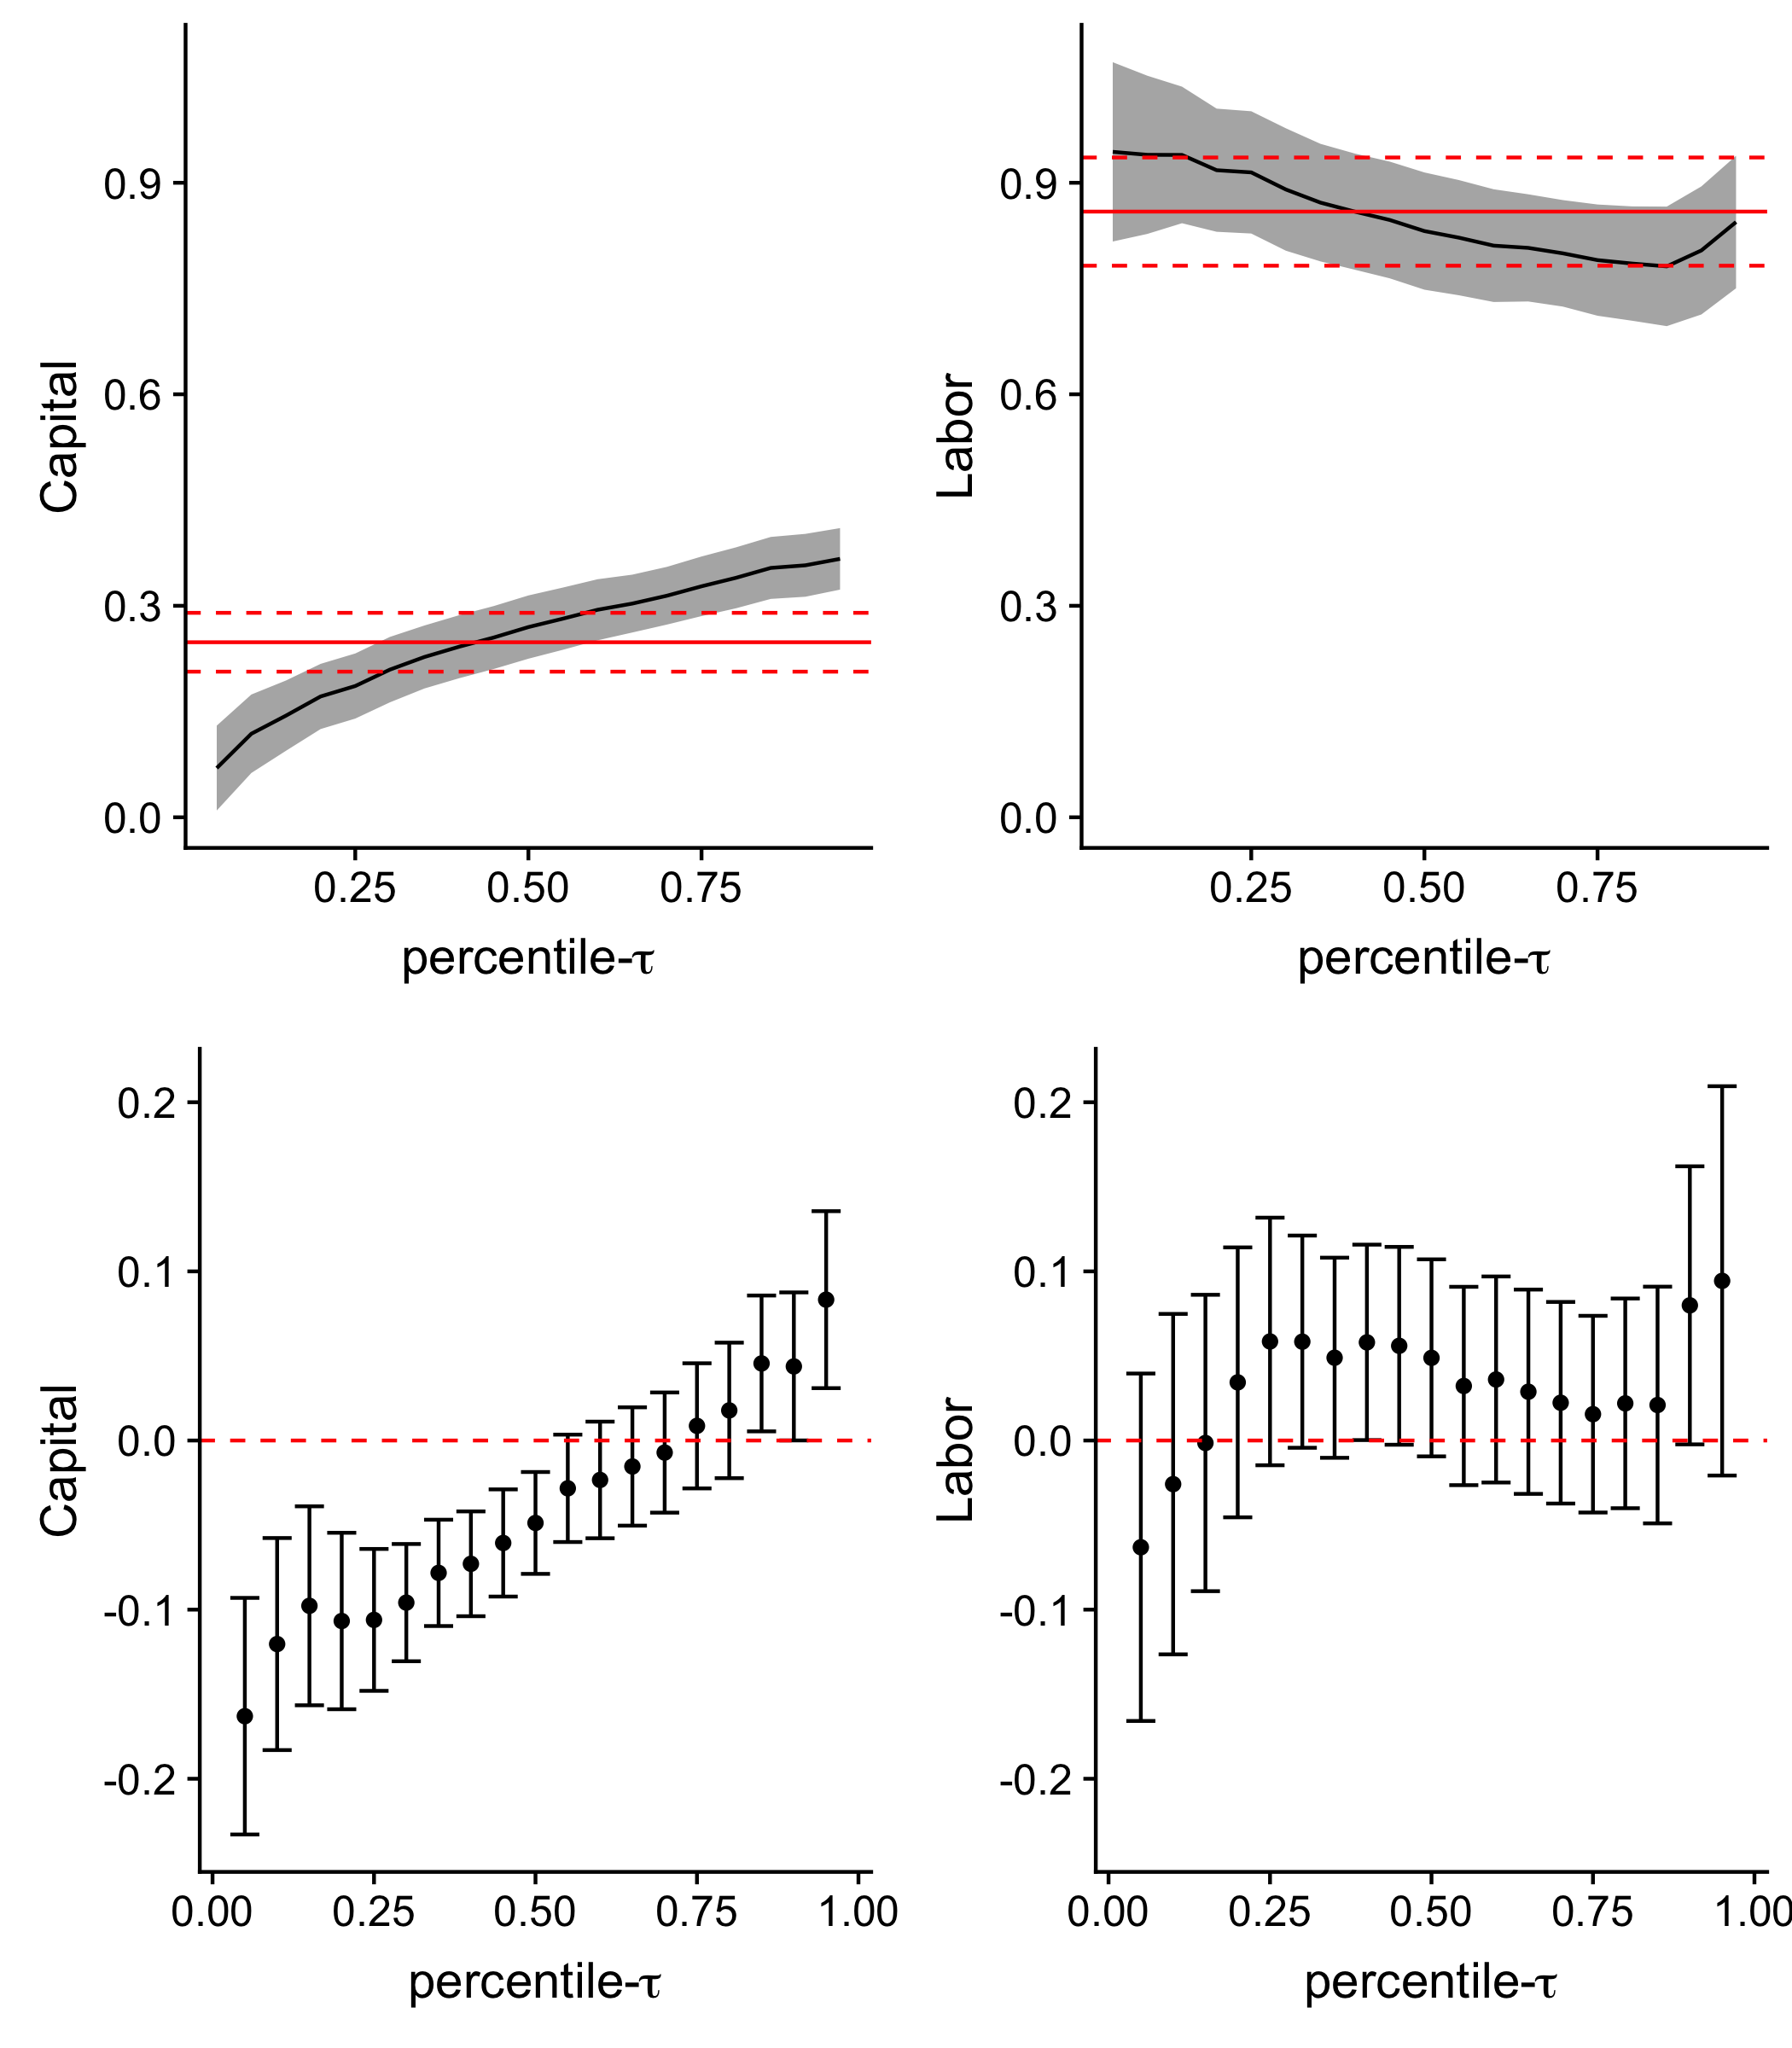
\includegraphics[width=8cm, height=8cm]{Chile/QACF_Coef_Plot_ISIC_321.png}
\caption*{\footnotesize $^{*}$Top row: Estimated values of production function coefficients and their point-wise 90\% confidence interval. Bottom row: Difference between DS and QR estimates that does not control for endogeneity and their 95\% confidence intervals.}
\label{fig:QACFCHL321}
\end{figure}

\begin{figure}[H]
\centering
\caption{Estimated Coefficients of Capital and Labor for all Chilean Manufacturing Plants}
\includegraphics[width=8cm, height=8cm]{Chile/QACF_Coef_Plot_ISIC_All.png}
\caption*{\footnotesize $^{*}$Top row: Estimated values of production function coefficients and their point-wise 90\% confidence interval. Bottom row: Difference between DS and QR estimates that does not control for endogeneity and their 95\% confidence intervals.}
\label{fig:QACFCHLall}
\end{figure}

\begin{table}[H]
\centering
\caption{Coefficient Estimates and Standard Errors for Chilean Manufacturing Plants}
\small
\begin{tabular}{cccccccccc}
  \hline\hline & & \multicolumn{2}{c}{Capital}  & \multicolumn{2}{c}{Labor} & \multicolumn{2}{c}{Returns to Scale} & \multicolumn{2}{c}{Capital Intensity}\\ \cmidrule(lr){3-4} \cmidrule(lr){5-6} \cmidrule(lr){7-8} \cmidrule(lr){9-10}ISIC & $\tau$ & Coef. & s.e & Coef. & s.e & Coef. & s.e & Coef. & s.e \\ 
  \hline
311 & 0.10 & 0.183 & 0.0249 & 0.447 & 0.0468 & 0.630 & 0.0321 & 0.410 & 0.0760 \\ 
   & 0.25 & 0.217 & 0.0228 & 0.530 & 0.0412 & 0.747 & 0.0298 & 0.410 & 0.0613 \\ 
   & 0.50 & 0.269 & 0.0224 & 0.552 & 0.0387 & 0.821 & 0.0279 & 0.487 & 0.0601 \\ 
   & 0.90 & 0.326 & 0.0235 & 0.654 & 0.0416 & 0.980 & 0.0292 & 0.498 & 0.0546 \\ 
  381 & 0.10 & 0.129 & 0.0380 & 0.728 & 0.0786 & 0.857 & 0.0535 & 0.178 & 0.0626 \\ 
   & 0.25 & 0.190 & 0.0328 & 0.740 & 0.0655 & 0.931 & 0.0469 & 0.257 & 0.0584 \\ 
   & 0.50 & 0.257 & 0.0318 & 0.699 & 0.0617 & 0.957 & 0.0447 & 0.368 & 0.0674 \\ 
   & 0.90 & 0.320 & 0.0344 & 0.738 & 0.0679 & 1.059 & 0.0473 & 0.434 & 0.0744 \\ 
  321 & 0.10 & 0.189 & 0.0387 & 0.692 & 0.0828 & 0.881 & 0.0578 & 0.273 & 0.0789 \\ 
   & 0.25 & 0.261 & 0.0325 & 0.674 & 0.0690 & 0.935 & 0.0522 & 0.387 & 0.0750 \\ 
   & 0.50 & 0.347 & 0.0330 & 0.588 & 0.0669 & 0.935 & 0.0502 & 0.591 & 0.0989 \\ 
   & 0.90 & 0.428 & 0.0328 & 0.584 & 0.0705 & 1.012 & 0.0537 & 0.734 & 0.1220 \\ 
  All & 0.10 & 0.281 & 0.0123 & 0.443 & 0.0251 & 0.724 & 0.0182 & 0.634 & 0.0441 \\ 
   & 0.25 & 0.357 & 0.0111 & 0.437 & 0.0217 & 0.795 & 0.0166 & 0.818 & 0.0444 \\ 
   & 0.50 & 0.421 & 0.0108 & 0.430 & 0.0200 & 0.851 & 0.0155 & 0.979 & 0.0468 \\ 
   & 0.90 & 0.486 & 0.0116 & 0.510 & 0.0221 & 0.996 & 0.0163 & 0.954 & 0.0453 \\ 
   \hline
\end{tabular}
\caption*{\footnotesize $^{*}$Standard errors are obtained using bootstrap with 500 replications. The first stage uses estimates from ACF.}
\label{CHLQACF}
\end{table}

\begin{table}[H]
\centering
\caption{ACF Coefficient Estimates and Standard Errors for Chilean Manufacturing Plants}
\small
\begin{tabular}{ccccccccc}
  \hline\hline & \multicolumn{2}{c}{Capital} & \multicolumn{2}{c}{Labor} & \multicolumn{2}{c}{Returns to Scale} & \multicolumn{2}{c}{Capital Intensity}\\ \cmidrule(lr){2-3} \cmidrule(lr){4-5} \cmidrule(lr){6-7} \cmidrule(lr){8-9}ISIC & Coef. & s.e & Coef. & s.e & Coef. & s.e & Coef. & s.e \\ 
  \hline
311 & 0.259 & 0.0222 & 0.550 & 0.0385 & 0.810 & 0.0280 & 0.471 & 0.0588 \\ 
  381 & 0.231 & 0.0323 & 0.734 & 0.0622 & 0.965 & 0.0447 & 0.315 & 0.0615 \\ 
  321 & 0.325 & 0.0319 & 0.615 & 0.0664 & 0.940 & 0.0508 & 0.528 & 0.0886 \\ 
  All & 0.398 & 0.0107 & 0.458 & 0.0202 & 0.855 & 0.0157 & 0.869 & 0.0418 \\ 
   \hline
\end{tabular}
\caption*{\footnotesize $^{*}$Standard errors are obtained using bootstrap with 500 replications.}
\label{CHLACF}
\end{table}

Figure \ref{fig:QACFCHLTFP} plots the densities of TFP for various quantiles and for ACF estimates. The plot shows significant differences between TFP estimates for low and high $\tau$, but similar densities of TFP from our estimator at $\tau=0.5$ to the mean estimates of ACF. Figure \ref{fig:QACFCHLTFPG} reports average productivity for each industry with base period set to 100. Productivity decreases in the beginning of the 1980s but then increases for the rest of the sample period. Similar to the US results, These estimates suggest that firms ranked lower on the conditional output distribution had higher productivity levels than higher ranked firms. The ACF estimates are similar to productivity of firms at $\tau=0.5$. These estimated results confirm that our estimator is useful to capture heterogeneous TFP across the conditional output distribution.

\begin{figure}[H]
	\centering
	\caption{DS and ACF Estimates of Log Total Factor Productivity}
	\includegraphics[width=11cm]{Chile/QACF_TFP_Plot.png}
	\caption*{\footnotesize $^{*}$Estimated Distributions of TFP from the DS estimator for $\tau \in \{0.1, 0.5, 0.9\}$ and those from  the ACF estimator.}
	\label{fig:QACFCHLTFP}
\end{figure}

\begin{figure}[H]
	\centering
	\caption{Chile Productivity Over Time}
	\includegraphics[width=11cm]{Chile/QACF_TFPgrowth_Plot.png}
	\caption*{\footnotesize $^{*}$Estimated average productivity (in levels) over time for Chile. Base year productivity is set to 100.}
	\label{fig:QACFCHLTFPG}
\end{figure}

Table \ref{QACFCHLTFPP} reports the estimated effects of firm characteristics on productivity using our estimator. For each $\tau$, we run a regression of the estimated productivity on the amount of firm exports, the amount of imported raw materials, and advertising expenditure, where all variables are log-transformed. Similarly, Table \ref{ACFCHLTFPP} provides the estimated effects using ACF. Our results show that the return to these activities diminish as $\tau$ increases, which estimates significant heterogeneous effects of firm characteristics across the conditional output distribution.  We also observe that there is not much difference between the median estimate $\tau=0.5$ and the mean estimates in Table \ref{ACFCHLTFPP}.

\begin{table}[H]
\centering
\caption{Productivity Differentials for Chilean Manufacturing Plants using DS}
\small
\begin{tabular}{cccccccc}
  \hline\hline & & \multicolumn{2}{c}{Exports}  & \multicolumn{2}{c}{Imports} & \multicolumn{2}{c}{Advertisements} \\ \cmidrule(lr){3-4} \cmidrule(lr){5-6} \cmidrule(lr){7-8}ISIC & $\tau$ & Coef. & s.e & Coef. & s.e & Coef. & s.e \\ 
  \hline
311 & 0.10 & 0.069 & 0.0377 & 0.184 & 0.0397 & 0.076 & 0.0279 \\ 
   & 0.25 & 0.057 & 0.0363 & 0.144 & 0.0384 & 0.054 & 0.0270 \\ 
   & 0.50 & 0.044 & 0.0358 & 0.120 & 0.0376 & 0.041 & 0.0268 \\ 
   & 0.90 & 0.026 & 0.0369 & 0.065 & 0.0374 & 0.012 & 0.0270 \\ 
  381 & 0.10 & 0.099 & 0.0299 & 0.192 & 0.0348 & 0.130 & 0.0377 \\ 
   & 0.25 & 0.068 & 0.0283 & 0.149 & 0.0354 & 0.105 & 0.0348 \\ 
   & 0.50 & 0.048 & 0.0275 & 0.122 & 0.0364 & 0.090 & 0.0332 \\ 
   & 0.90 & 0.010 & 0.0277 & 0.069 & 0.0388 & 0.058 & 0.0338 \\ 
  321 & 0.10 & 0.021 & 0.0278 & 0.044 & 0.0374 & 0.074 & 0.0327 \\ 
   & 0.25 & 0.005 & 0.0276 & 0.018 & 0.0366 & 0.056 & 0.0317 \\ 
   & 0.50 & 0.007 & 0.0283 & 0.017 & 0.0371 & 0.055 & 0.0323 \\ 
   & 0.90 & -0.017 & 0.0297 & -0.020 & 0.0399 & 0.030 & 0.0350 \\ 
  All & 0.10 & 0.101 & 0.0118 & 0.192 & 0.0155 & 0.143 & 0.0121 \\ 
   & 0.25 & 0.073 & 0.0116 & 0.156 & 0.0151 & 0.124 & 0.0116 \\ 
   & 0.50 & 0.049 & 0.0116 & 0.127 & 0.0150 & 0.109 & 0.0114 \\ 
   & 0.90 & 0.005 & 0.0117 & 0.067 & 0.0151 & 0.073 & 0.0116 \\ 
   \hline
\end{tabular}
\caption*{\footnotesize $^{*}$Standard errors are obtained using bootstrap with 500 replications. Log(TFP) is regressed on log(Exports), log(Imports), and log(Advertisements).}
\label{QACFCHLTFPP}
\end{table}

\begin{table}[H]
\centering
\caption{Productivity Differentials for Chilean Manufacturing Plants using ACF}
\small
\begin{tabular}{ccccccc}
  \hline\hline & \multicolumn{2}{c}{Exports}  & \multicolumn{2}{c}{Imports} & \multicolumn{2}{c}{Advertisements} \\ \cmidrule(lr){2-3} \cmidrule(lr){4-5} \cmidrule(lr){6-7}ISIC & Coef. & s.e & Coef. & s.e & Coef. & s.e \\ 
  \hline
311 & 0.046 & 0.0359 & 0.123 & 0.0377 & 0.043 & 0.0269 \\ 
  381 & 0.051 & 0.0278 & 0.126 & 0.0362 & 0.092 & 0.0338 \\ 
  321 & 0.005 & 0.0277 & 0.015 & 0.0366 & 0.054 & 0.0322 \\ 
  All & 0.052 & 0.0116 & 0.129 & 0.0149 & 0.109 & 0.0115 \\ 
   \hline
\end{tabular}
\caption*{\footnotesize $^{*}$Standard errors are obtained using bootstrap with 500 replications. Log(TFP) is regressed on log(Exports), log(Imports), and log(Advertisements).}
\label{ACFCHLTFPP}
\end{table}

%------------------------------------------------------------------------------------------------

\subsection{Colombian Manufacturing}
This data comes from the Colombian manufacturing census conducted by the Departamento Administrativo Nacional de Estadistica. The sample is collected between 1977 and 1991. We divide our estimates into the three largest manufacturing industries: Food (ISIC 311), Apparel (ISIC 322), and Fabricated Metals (ISIC 381). As we did with the Chilean sample, we also aggregate the three industries with other smaller industries to obtain estimates from the entire sample of manufacturing plants. Summary statistics for this data is provided in Appendix \ref{COLdata} in Table \ref{COLsum}.

Figures \ref{fig:QACFCOL311}, \ref{fig:QACFCOL321}, \ref{fig:QACFCOL381}, and \ref{fig:QACFCOLall}  illustrate the estimates from our model compared to ACF estimates (top row) as well as the differences between our model and QR estimates that does not control for endogeneity (bottom row). The capital estimates in each industry are increasing and the labor estimates are decreasing in $\tau$. In all manufacturing industries and the combined sample except ISIC 381 are capital estimates different from ACF for both low and high percentiles. In each industry the magnitude of the differences between low an high $\tau$ is quite large. In ISIC 311, capital estimates range from 0.242 to 0.563 and labor estimates range from 0.567 to 0.323. In ISIC 322, capital estimates range from 0.25 to 0.7 and labor estimates range from 0.75 to 0.47. In ISIC 381, capital estimates range from 0.247 to 0.538 and labor estimates range from 0.603 to 0.391. Lastly, in the combined sample, capital estimates range from 0.258 to 0.578 and labor estimates range from 0.585 to 0.4. Comparing our results to those obtained using QR that does not control for endogeneity, most of the differences appear through the labor estimates which is intuitive as labor is more correlated to current productivity than capital. Using the estimates of capital and labor elasticities, we construct measures of returns to scale and capital intensity for each industry in Table \ref{COLQACF}. Table \ref{COLACF} reports the mean estimates from ACF. Most firms experience constant or slightly decreasing returns to scale. Returns to scale are smallest in ISIC 311. It is interesting to note that both returns to scale and capital intensity are increasing in $\tau$.

\begin{figure}[H]
\centering
\caption{Estimated Coefficients of Capital and Labor for Colombia: ISIC 311}
\includegraphics[width=8cm, height=8cm]{Colombia/QACF_Coef_Plot_ISIC_311.png}
\caption*{\footnotesize $^{*}$Top row: Estimated values of production function coefficients and their point-wise 90\% confidence interval. Bottom row: Difference between DS and QR estimates that does not control for endogeneity and their 95\% confidence intervals.}
\label{fig:QACFCOL311}
\end{figure}

\begin{figure}[H]
\centering
\caption{Estimated Coefficients of Capital and Labor for Colombia: ISIC 322}
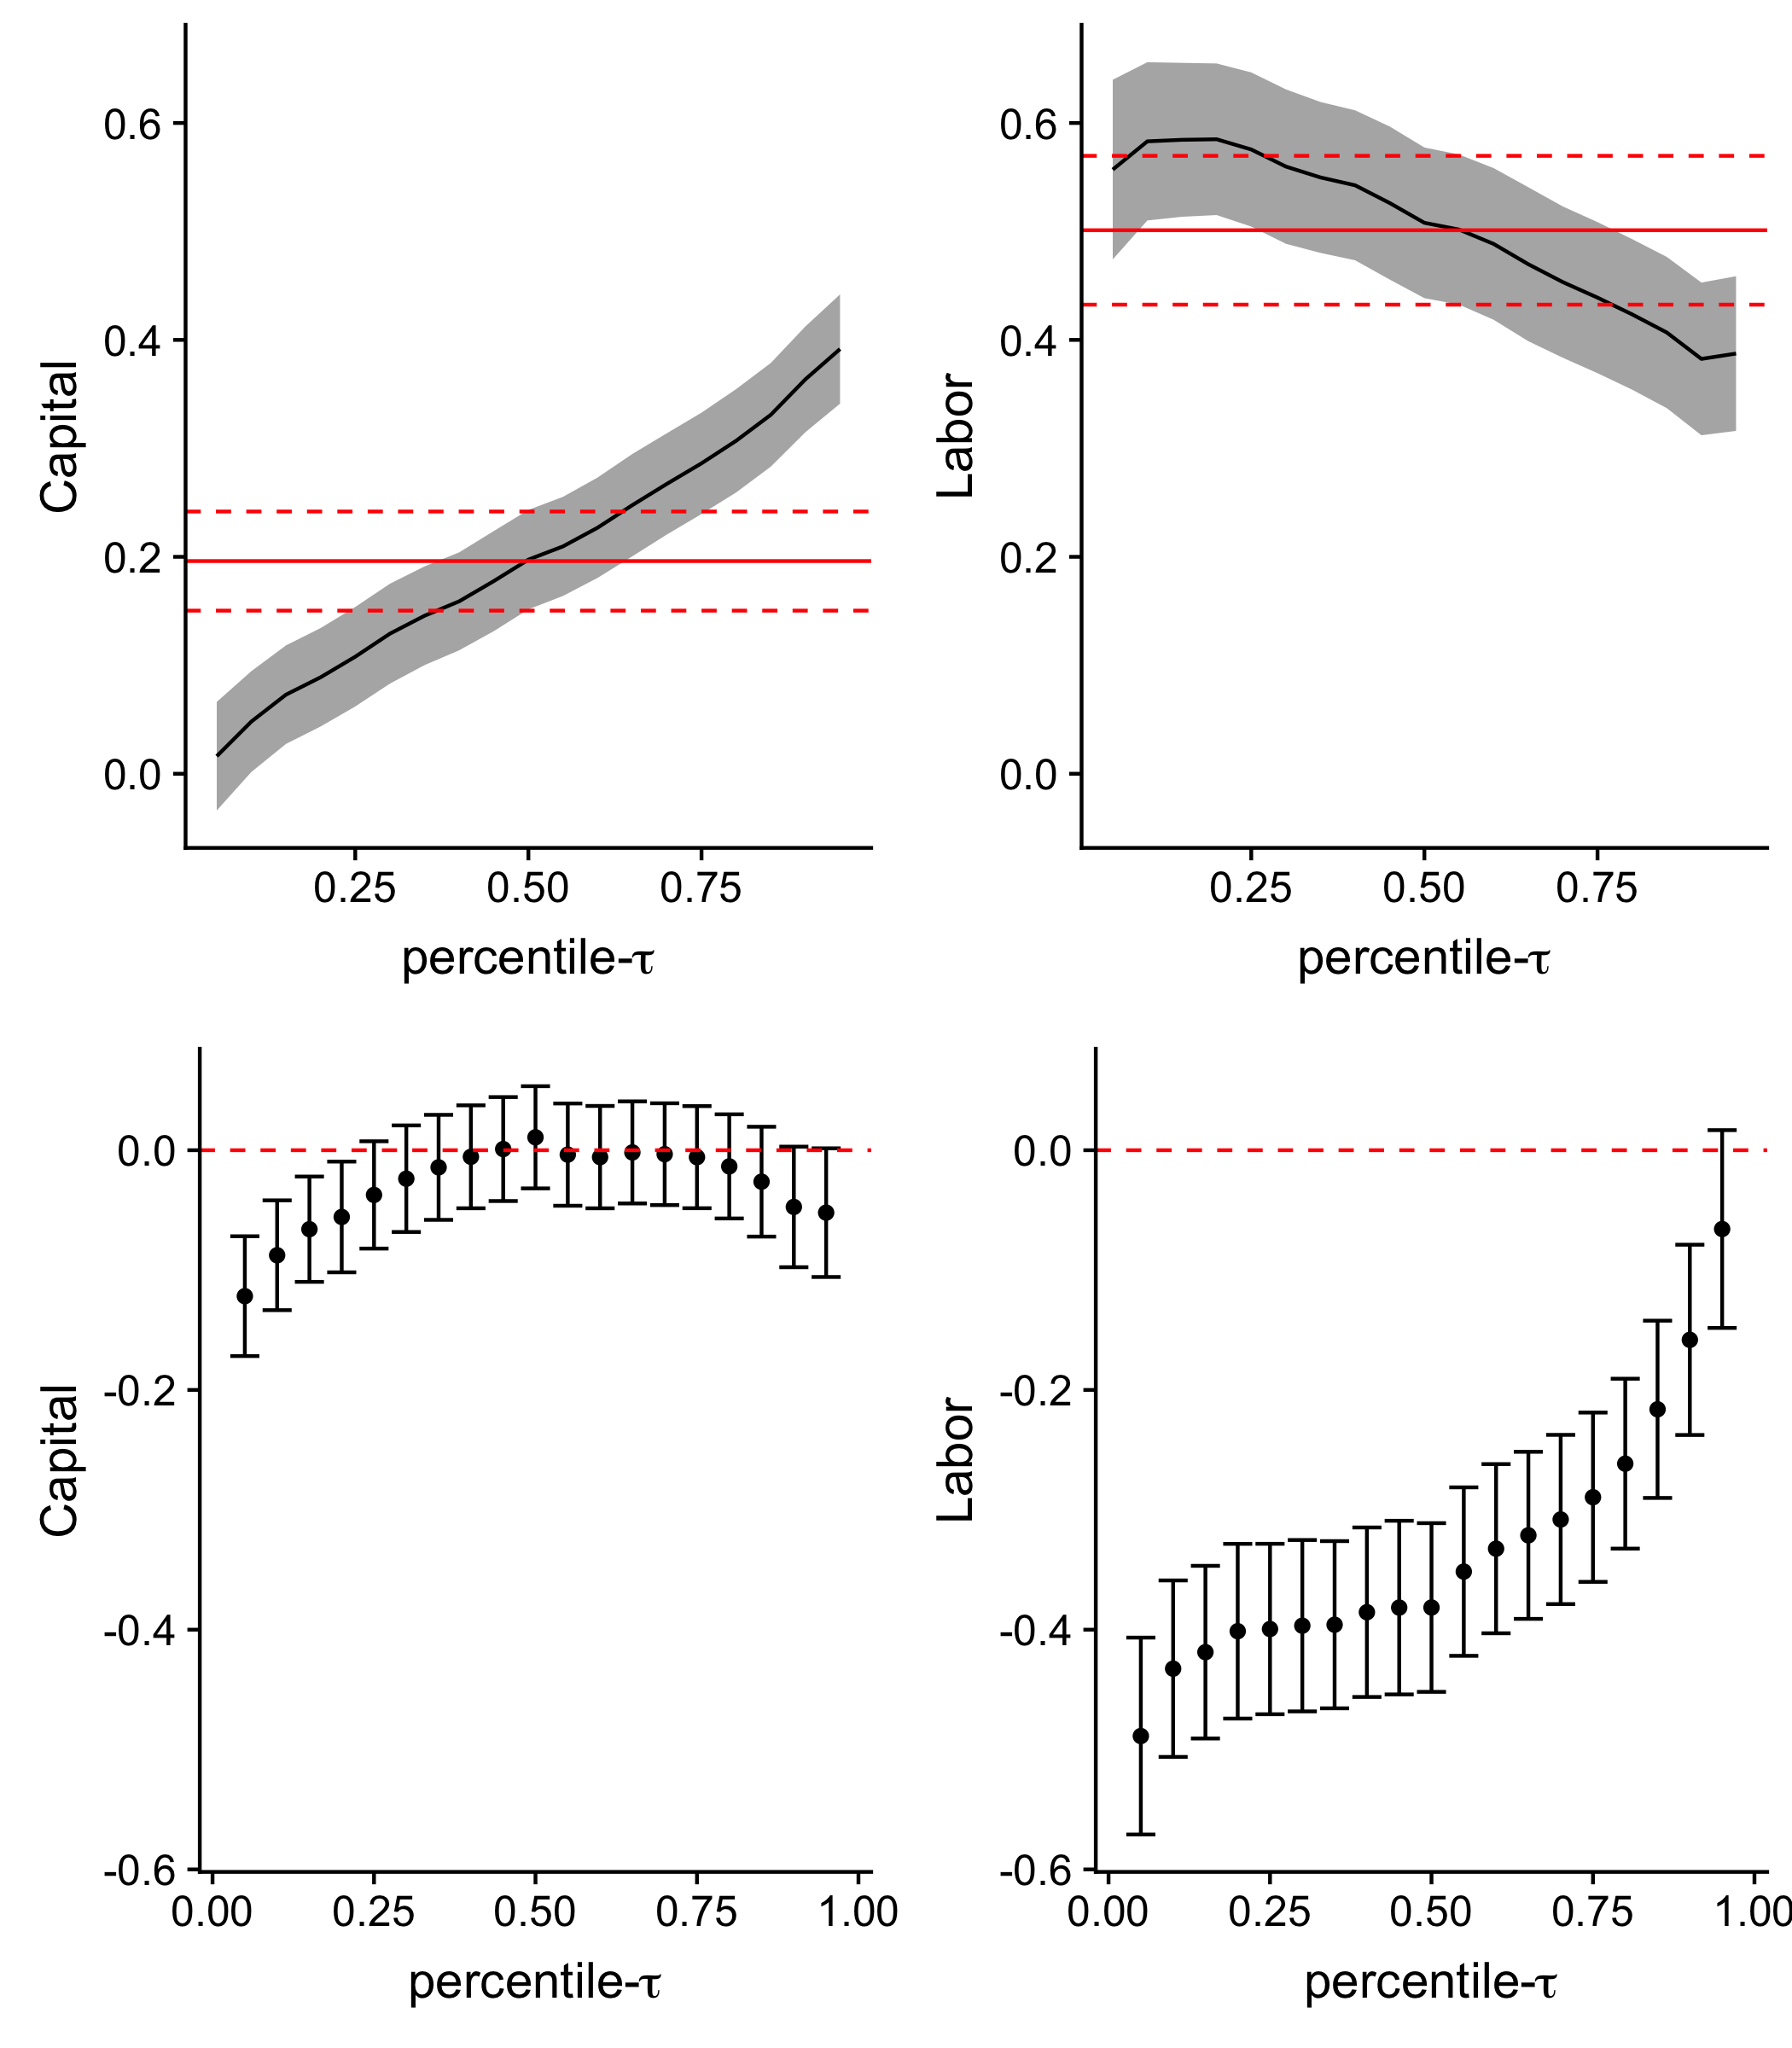
\includegraphics[width=8cm, height=8cm]{Colombia/QACF_Coef_Plot_ISIC_322.png}
\caption*{\footnotesize $^{*}$Top row: Estimated values of production function coefficients and their point-wise 90\% confidence interval. Bottom row: Difference between DS and QR estimates that does not control for endogeneity and their 95\% confidence intervals.}
\label{fig:QACFCOL321}
\end{figure}

\begin{figure}[H]
\centering
\caption{Estimated Coefficients of Capital and Labor for Colombia: ISIC 381}
\includegraphics[width=8cm, height=8cm]{Colombia/QACF_Coef_Plot_ISIC_381.png}
\caption*{\footnotesize $^{*}$Top row: Estimated values of production function coefficients and their point-wise 90\% confidence interval. Bottom row: Difference between DS and QR estimates that does not control for endogeneity and their 95\% confidence intervals.}
\label{fig:QACFCOL381}
\end{figure}

\begin{figure}[H]
\centering
\caption{Estimated Coefficients of Capital and Labor for all Colombian Manufacturing Plants}
\includegraphics[width=8cm, height=8cm]{Colombia/QACF_Coef_Plot_ISIC_All.png}
\caption*{\footnotesize $^{*}$Top row: Estimated values of production function coefficients and their point-wise 90\% confidence interval. Bottom row: Difference between DS and QR estimates that does not control for endogeneity and their 95\% confidence intervals.}
\label{fig:QACFCOLall}
\end{figure}

\begin{table}[H]
\centering
\caption{Coefficient Estimates and Standard Errors for Colombian Manufacturing Plants}
\small
\begin{tabular}{cccccccccc}
  \hline\hline & & \multicolumn{2}{c}{Capital}  & \multicolumn{2}{c}{Labor} & \multicolumn{2}{c}{Returns to Scale} & \multicolumn{2}{c}{Capital Intensity}\\ \cmidrule(lr){3-4} \cmidrule(lr){5-6} \cmidrule(lr){7-8} \cmidrule(lr){9-10}ISIC & $\tau$ & Coef. & s.e & Coef. & s.e & Coef. & s.e & Coef. & s.e \\ 
  \hline
311 & 0.10 & 0.242 & 0.0551 & 0.567 & 0.0621 & 0.809 & 0.0391 & 0.427 & 0.1058 \\ 
   & 0.25 & 0.314 & 0.0555 & 0.536 & 0.0594 & 0.851 & 0.0352 & 0.586 & 0.1221 \\ 
   & 0.50 & 0.393 & 0.0562 & 0.472 & 0.0600 & 0.865 & 0.0344 & 0.831 & 0.1575 \\ 
   & 0.90 & 0.563 & 0.0562 & 0.323 & 0.0626 & 0.886 & 0.0368 & 1.746 & 0.3270 \\ 
  322 & 0.10 & 0.331 & 0.0461 & 0.741 & 0.0741 & 1.071 & 0.0544 & 0.446 & 0.0902 \\ 
   & 0.25 & 0.427 & 0.0419 & 0.681 & 0.0641 & 1.107 & 0.0508 & 0.627 & 0.1011 \\ 
   & 0.50 & 0.530 & 0.0419 & 0.577 & 0.0614 & 1.107 & 0.0489 & 0.920 & 0.1409 \\ 
   & 0.90 & 0.675 & 0.0458 & 0.478 & 0.0670 & 1.153 & 0.0489 & 1.413 & 0.2480 \\ 
  381 & 0.10 & 0.247 & 0.0655 & 0.603 & 0.0919 & 0.850 & 0.0687 & 0.409 & 0.1910 \\ 
   & 0.25 & 0.330 & 0.0659 & 0.542 & 0.0901 & 0.872 & 0.0668 & 0.609 & 0.2568 \\ 
   & 0.50 & 0.404 & 0.0656 & 0.482 & 0.0886 & 0.886 & 0.0660 & 0.839 & 0.3616 \\ 
   & 0.90 & 0.538 & 0.0670 & 0.391 & 0.0939 & 0.929 & 0.0679 & 1.377 & 0.7882 \\ 
  All & 0.10 & 0.258 & 0.0206 & 0.585 & 0.0325 & 0.843 & 0.0191 & 0.442 & 0.0494 \\ 
   & 0.25 & 0.345 & 0.0205 & 0.551 & 0.0317 & 0.895 & 0.0185 & 0.626 & 0.0602 \\ 
   & 0.50 & 0.424 & 0.0207 & 0.499 & 0.0318 & 0.923 & 0.0183 & 0.849 & 0.0780 \\ 
   & 0.90 & 0.578 & 0.0205 & 0.400 & 0.0313 & 0.978 & 0.0182 & 1.447 & 0.1311 \\ 
   \hline
\end{tabular}
\caption*{\footnotesize $^{*}$Standard errors are obtained using bootstrap with 500 replications. The first stage uses estimates from ACF}
\label{COLQACF}
\end{table}

\begin{table}[H]
\centering
\caption{ACF Coefficient Estimates and Standard Errors for Colombian Manufacturing Plants}
\small
\begin{tabular}{ccccccccc}
  \hline\hline & \multicolumn{2}{c}{Capital} & \multicolumn{2}{c}{Labor} & \multicolumn{2}{c}{Returns to Scale} & \multicolumn{2}{c}{Capital Intensity}\\ \cmidrule(lr){2-3} \cmidrule(lr){4-5} \cmidrule(lr){6-7} \cmidrule(lr){8-9}ISIC & Coef. & s.e & Coef. & s.e & Coef. & s.e & Coef. & s.e \\ 
  \hline
311 & 0.403 & 0.0550 & 0.442 & 0.0576 & 0.845 & 0.0346 & 0.911 & 0.1660 \\ 
  322 & 0.506 & 0.0421 & 0.608 & 0.0629 & 1.114 & 0.0497 & 0.831 & 0.1279 \\ 
  381 & 0.414 & 0.0656 & 0.452 & 0.0869 & 0.866 & 0.0647 & 0.917 & 0.4060 \\ 
  All & 0.423 & 0.0197 & 0.484 & 0.0298 & 0.908 & 0.0177 & 0.874 & 0.0765 \\ 
   \hline
\end{tabular}
\caption*{\footnotesize $^{*}$Standard errors are obtained using bootstrap with 500 replications.}
\label{COLACF}
\end{table}

Figure \ref{fig:QACFCOLTFP} plots the densities of TFP for various quantiles and for ACF estimates. Compared to the U.S. and Chile, there is less dispersion between these estimates across $\tau$. Figure \ref{fig:QACFCOLTFPG} reports average productivity for each industry with base period set to 100. Productivity decreases in late 1970s and early 1980s for ISIC 311, 381, and the combined sample but then increases for the rest of the sample period. Productivity in ISIC 322 has increased over time, whereas productivity in ISIC 381 has mostly decreased. The ACF estimates are similar to productivity of firms at $\tau=0.5$. 

\begin{figure}[H]
\centering
\caption{DS and ACF Estimates of Log Total Factor Productivity}
\includegraphics[width=11cm]{Colombia/QACF_TFP_Plot.png}
\caption*{\footnotesize $^{*}$Estimated distributions of TFP from the DS estimator for $\tau \in \{0.1, 0.5, 0.9\}$ and those from  the ACF estimator.}
\label{fig:QACFCOLTFP}
\end{figure}

\begin{figure}[H]
\centering
\caption{Colombia Productivity Over Time}
\includegraphics[width=11cm]{Colombia/QACF_TFPgrowth_Plot.png}
\caption*{\footnotesize $^{*}$Estimated average productivity (in levels) over time for Colombia. Base year productivity is set to 100.}
\label{fig:QACFCOLTFPG}
\end{figure}

Table \ref{QACFCOLTFPP} estimates the effects of firm characteristics on productivity. Similar to the Chilean estimates, our results show that the returns to these activities diminish as $\tau$ increases, which confirms significant heterogeneous effects of firm characteristics across the conditional output distribution. There is not much difference between the median estimate $\tau=0.5$ and the mean estimates in Table \ref{ACFCOLTFPP}. Some estimates in ISIC 322 are negative, but these are not statistically significant.

\begin{table}[H]
\centering
\caption{Productivity Differentials for Colombian Manufacturing Plants using DS}
\small
\begin{tabular}{cccccccc}
  \hline\hline & & \multicolumn{2}{c}{Exports}  & \multicolumn{2}{c}{Imports} & \multicolumn{2}{c}{Advertisements} \\ \cmidrule(lr){3-4} \cmidrule(lr){5-6} \cmidrule(lr){7-8}ISIC & $\tau$ & Coef. & s.e & Coef. & s.e & Coef. & s.e \\ 
  \hline
311 & 0.10 & 0.090 & 0.0323 & 0.208 & 0.0420 & 0.158 & 0.0350 \\ 
   & 0.25 & 0.074 & 0.0308 & 0.194 & 0.0387 & 0.151 & 0.0324 \\ 
   & 0.50 & 0.061 & 0.0301 & 0.186 & 0.0353 & 0.149 & 0.0301 \\ 
   & 0.90 & 0.034 & 0.0300 & 0.171 & 0.0305 & 0.145 & 0.0271 \\ 
  322 & 0.10 & 0.002 & 0.0243 & 0.040 & 0.0294 & 0.057 & 0.0254 \\ 
   & 0.25 & -0.010 & 0.0230 & 0.015 & 0.0291 & 0.036 & 0.0253 \\ 
   & 0.50 & -0.017 & 0.0225 & -0.000 & 0.0298 & 0.020 & 0.0258 \\ 
   & 0.90 & -0.034 & 0.0223 & -0.035 & 0.0319 & -0.011 & 0.0274 \\ 
  381 & 0.10 & 0.107 & 0.0384 & 0.158 & 0.0424 & 0.169 & 0.0372 \\ 
   & 0.25 & 0.091 & 0.0372 & 0.141 & 0.0407 & 0.151 & 0.0362 \\ 
   & 0.50 & 0.079 & 0.0364 & 0.128 & 0.0394 & 0.136 & 0.0354 \\ 
   & 0.90 & 0.051 & 0.0347 & 0.099 & 0.0369 & 0.106 & 0.0341 \\ 
  All & 0.10 & 0.087 & 0.0118 & 0.176 & 0.0117 & 0.157 & 0.0096 \\ 
   & 0.25 & 0.068 & 0.0111 & 0.148 & 0.0113 & 0.136 & 0.0093 \\ 
   & 0.50 & 0.053 & 0.0106 & 0.126 & 0.0111 & 0.122 & 0.0091 \\ 
   & 0.90 & 0.025 & 0.0099 & 0.085 & 0.0110 & 0.094 & 0.0091 \\ 
   \hline
\end{tabular}
\caption*{\footnotesize $^{*}$Standard errors are obtained using bootstrap with 500 replications. Log(TFP) is regressed on log(Exports), log(Imports), and log(Advertisements).}
\label{QACFCOLTFPP}
\end{table}

\begin{table}[H]
\centering
\caption{Productivity Differentials for Colombian Manufacturing Plants using ACF}
\small
\begin{tabular}{ccccccc}
  \hline\hline & \multicolumn{2}{c}{Exports}  & \multicolumn{2}{c}{Imports} & \multicolumn{2}{c}{Advertisements} \\ \cmidrule(lr){2-3} \cmidrule(lr){4-5} \cmidrule(lr){6-7}ISIC & Coef. & s.e & Coef. & s.e & Coef. & s.e \\ 
  \hline
311 & 0.063 & 0.0303 & 0.190 & 0.0349 & 0.152 & 0.0301 \\ 
  322 & -0.016 & 0.0225 & 0.002 & 0.0296 & 0.023 & 0.0256 \\ 
  381 & 0.082 & 0.0363 & 0.133 & 0.0391 & 0.140 & 0.0352 \\ 
  All & 0.056 & 0.0106 & 0.130 & 0.0112 & 0.125 & 0.0091 \\ 
   \hline
\end{tabular}
\label{ACFCOLTFPP}
\caption*{\footnotesize $^{*}$Standard errors are obtained using bootstrap with 500 replications. Log(TFP) is regressed on log(Exports), log(Imports), and log(Advertisements).}
\end{table}

\section{Conclusions} \label{conclusion}

We propose a method that extends the control function approach to estimating the conditional quantiles of firm output. The method is computationally attractive, as it resembles many two-stage estimators used in quantile regression models such as \cite{Lee2007} or \cite{Chernozhukov2005}. As a result, practitioners can easily apply the proposed estimator to production function models where the data may reveal significant heterogeneous output elasticities along the conditional distribution. We showed that this estimator works well in finite samples and showed that it captures heterogeneity under different data generating processes. An application to widely used datasets from the U.S., Chile, and Colombia showed that in some industries, our estimator captures unobserved heterogeneity that the ACF estimator does not.

Improvements and extensions of this estimator are currently being explored. For example, using a value-added production function may show more heterogeneity in estimates of elasticities and productivity than a gross-output production function. However, using a gross-output production function with an intermediate input proxy variable suffers from non-identification. An adaption to the approach of \cite{Gandhi2020} is not as straightforward. This paper also makes a brief connection between the literature on production risk and quantile utility maximization. Currently, quantile utility maximization problems and estimation of these models are being studied by \cite{Castro2019} in the context of dynamic consumption problems. It would be interesting to explore a model for a firm who maximizes quantile utility of profits which could provide a structural interpretation for unobserved heterogeneity that are obtained from quantile regression estimates.

This paper contributes to the growing literature on production functions with unobserved heterogeneity. We show that differences in firm output correspond to the the rank of the ex-post shock. The location-shift model for productivity we propose here restricts us from examining other dimensions of firm heterogeneity. Therefore, allowing richer distributional effects of productivity would be an interesting extension. This approach also restricts us from examining non-Hicks neutral productivity shocks such as factor-augmenting productivity. We are currently working on an extension of this paper to a non-separable model to address these last two points, but the estimator we propose here is computationally attractive and easy to implement in empirical research.    

\pagebreak
\newpage


%\section*{Appendix}
%\appendix
%\begin{Large}
%\noindent \textbf{A. Proof of the Theorems}
%\end{Large}

%\counterwithin{theorem}{section}
%\section{Proofs}





\bibliographystyle{ecca.bst}
\bibliography{references}{}

\pagebreak
\newpage
\section*{Appendix}
\begin{appendices}

\section{Identification} \label{identification}

\textit{Proof of Theorem \ref{idtheorem}}:\\
We first note that the conditional quantile function is given by
\begin{equation} \label{charQ}
Q_{\tau}(Z_{it}|x_{i})=Q_{\tau}(x_{it}\boldsymbol\beta(\eta_{it})|x_{i})=x_{it}\boldsymbol\beta(\tau),
\end{equation}
where the second equality follows from Assumption \eqref{idpart1}(d).
Since the conditional quantiles are the inverse of the conditional distribution functions, identification of parameters $\boldsymbol\beta(\tau)$ comes from identification of the conditional distribution functions.

Using the result of \cite{g}, the conditional distributions of $Z_{it}|x_{i}$ can be recovered as follows:
\begin{equation} \label{charCDF}
F_{Z_{it}|x_{i}}(Z_{it}|x_{i})=\frac{1}{2}-\underset{\upsilon\rightarrow \infty}{\operatorname{lim}}\int_{-\upsilon}^{\upsilon}\frac{e^{-\mathrm{i}sZ_{it}}}{2\pi \mathrm{i}s}\phi_{Z_{it}|x_{i}}(s|x_{i})ds.
\end{equation}
As a result, identification of the conditional characteristic function $\phi_{Z_{it}|x_{i}}(s|x_{i})$ is sufficient to guarantee identification of the parameters.

Recall that for any random variable $X$ and $\rho\neq 0$, let $\tilde{X}=X/\rho$. Using Assumption \ref{idpart1}(b)(i)-(ii) we can write the conditional characteristic function of $Y_{it}|x_{i}$ as
\begin{equation} \label{repchar1}
\begin{split}
\phi_{Y_{it}|x_{i}}(s|x_{i})&=\mathbbm{E}[\exp\{\mathrm{i}[s(Z_{it}+\omega_{it}])\}|x_{i}]\\
&=\mathbbm{E}[\exp\{\mathrm{i}sZ_{it}\}|x_{i}]\mathbbm{E}[\exp\{\mathrm{i}s\omega_{it}\}|x_{i}]\\
&=\phi_{Z_{it}|x_{i}}(s|x_{i})\phi_{\omega_{it}|x_{i}}(s|x_{i}).
\end{split}
\end{equation}
The characteristic function of $(Y_{it}, \tilde{Y}_{it+1})$ conditional on $X_{i}=x_{i}$ can then be written as:
\begin{equation*} \label{jointchar}
\begin{split}
&\Psi_{(Y_{it}, \tilde{Y}_{it+1})|x_{i}}(s_{1}, s_{2}|x_{i})\\
=&\mathbbm{E}[\exp\{\mathrm{i}[s_{1}Y_{it}+s_{2}\tilde{Y}_{it+1}]\}|x_{i}]\\
=&\mathbbm{E}[\exp\{\mathrm{i}[s_{1}Z_{it}+s_{1}\omega_{it}+s_{2}Z_{it+1}+s_{2}\omega_{it+1}]\}|x_{i}]\\
=&\mathbbm{E}[\exp\{\mathrm{i}[s_{1}Z_{it}+s_{2}\tilde{Z}_{it+1}+s_{2}\tilde{\xi}_{it+1}+(s_{1}+s_{2})\omega_{it}]\}|x_{i}]\\
=&\mathbbm{E}[\exp\{\mathrm{i}s_{1}Z_{it}\}|x_{i}]\mathbbm{E}[\exp\{\mathrm{i}[s_{2}\tilde{Z}_{it+1}+s_{2}\tilde{\xi}_{it+1}+(s_{1}+s_{2})\omega_{it}]\}|x_{i}]\\
=&\mathbbm{E}[\exp\{\mathrm{i}s_{1}Z_{it}\}|x_{i}]\mathbbm{E}[\exp\{\mathrm{i}s_{2}\tilde{Z}_{it+1}\}|x_{i}]\mathbbm{E}[\exp\{\mathrm{i}[s_{2}\tilde{\xi}_{it+1}+(s_{1}+s_{2})\omega_{it}]\}|x_{i}]
\end{split}
\end{equation*}
\begin{equation}
\begin{split}
=&\mathbbm{E}[\exp\{\mathrm{i}s_{1}Z_{it}\}|x_{i}]\mathbbm{E}[\exp\{\mathrm{i}s_{2}\tilde{Z}_{it+1}\}|x_{i}]\mathbbm{E}[\exp\{\mathrm{i}s_{2}\tilde{\xi}_{it+1}\}|x_{i}]\mathbbm{E}[\exp\{\mathrm{i}(s_{1}+s_{2})\omega_{it}]\}|x_{i}]\\
=&\phi_{Z_{it}|x_{i}}(s_{1}|x_{i})\phi_{\tilde{Z}_{it+1}|x_{i}}(s_{2}|x_{i})\phi_{\tilde{\xi}_{it+1}|x_{i}}(s_{2}|x_{i})\phi_{\omega_{it}|x_{i}}((s_{1}+s_{2})|x_{i}),
\end{split}
\end{equation}
where the third equality uses the Markov process for productivity and the fourth, fifth, and sixth equality use Assumption \ref{idpart1}(b)(i), (ii), and (iii), respectively. Taking the derivative of \eqref{jointchar} with respect to its first component yields
\begin{equation} \label{jointchard}
\begin{split}
&\partial_{s_{1}}\Psi_{(y_{it}, \tilde{y}_{it+1})|x_{i}}(s_{1}, s_{2}|x_{i})\\
=&\partial_{s_{1}}\phi_{Z_{it}|x_{i}}(s_{1}|x_{i})\phi_{\tilde{Z}_{it+1}|x_{i}}(s_{2}|x_{i})\phi_{\tilde{\xi}_{it+1}|x_{i}}(s_{2}|x_{i})\phi_{\omega_{it}|x_{i}}((s_{1}+s_{2})|x_{i})\\
&+\phi_{Z_{it}|x_{i}}(s_{1}|x_{i})\phi_{\tilde{Z}_{it+1}|x_{i}}(s_{2}|x_{i})\phi_{\tilde{\xi}_{it+1}|x_{i}}(s_{2}|x_{i})\partial_{s_{1}}\phi_{\omega_{it}|x_{i}}(s_{1}+s_{2}|x_{i}).
\end{split}
\end{equation}
Dividing Equation \eqref{jointchard} by \eqref{jointchar} we obtain:
\begin{equation*}
\begin{split}
\frac{\partial_{s_{1}}\Psi_{(y_{it}, \tilde{y}_{it+1})|x_{i}}(s_, -s|x_{i})}{\Psi_{(y_{it}, \tilde{y}_{it+1})|x_{i}}(s, -s|x_{i})}=&\frac{\phi^{'}_{Z_{it}|x_{i}}(s|x_{i})}{\phi_{Z_{it}|x_{i}}(s|x_{i})}+\frac{\phi^{'}_{\omega_{it}|x_{i}}(0|x_{i})}{\phi_{\omega_{it}|x_{i}}(0|x_{i})}\\
=&\frac{\phi^{'}_{Z_{it}|x_{i}}(s|x_{i})}{\phi_{Z_{it}|x_{i}}(s|x_{i})}+\mathrm{i}\mathbbm{E}[\omega_{it}|x_{i}],
\end{split}
\end{equation*}
provided that the conditional characteristic functions are non-vanishing according to Assumption \ref{idpart1}(c). The second equality follows from the fact that $\phi_{\omega_{it}|x_{i}}(0|x_{i})=1$ and $\phi^{'}_{\omega_{it}|x_{i}}(0|x_{i})=\mathrm{i}\mathbbm{E}[\omega_{it}|x_{i}]$ by properties of characteristic functions. We first discuss identification of $\mathbbm{E}[\omega_{it}|x_{i}]$. Note that,
\begin{equation*}
\begin{split}
\mathbbm{E}[\omega_{it}|x_{i}]&=\mathbbm{E}[y_{it}-Z_{it}|x_{i}]=\mathbbm{E}[y_{it}-x_{it}\beta(\eta_{it})|x_{i}]=\mathbbm{E}[y_{it}|x_{i}]-x_{it}\mathbbm{E}[\beta(\eta_{it})|x_{i}]\\
&=\mathbbm{E}[y_{it}|x_{i}]-x_{it}\mathbbm{E}[\beta(\eta_{it})]=\mathbbm{E}[y_{it}|x_{i}]-x_{it}\boldsymbol{\beta}^{\mu},
\end{split}
\end{equation*}
where the fourth equality follows from the independence assumption in \eqref{idpart1}(d). In order to identify $\mathbbm{E}[\omega_{it}|x_{i}]$, we must identify $\boldsymbol{\beta}^{\mu}$. This is satisfied by Assumption \ref{idpart2}(f). Then the conditional characteristic function $\phi_{Z_{it}|x_{i}}(s|x_{i})$ is identified through
\begin{equation}\label{charZ1}
\phi_{Z_{it}|x_{i}}(s|x_{i})=\exp\Bigg(\int_{0}^{s}\frac{\mathrm{i}\mathbbm{E}[y_{it}\exp(\mathrm{i}\gamma(y_{it}-\tilde{y}_{it+1}))|x_{i}]}{\phi_{y_{it}-\tilde{y}_{it+1}|x_{i}}(\gamma|x_{i})}d\gamma-\mathrm{i}s\mathbbm{E}[\omega_{it}|x_{i}]\Bigg),
\end{equation}
given that $\rho$ is also identified from Assumption \ref{idpart2}(f). To identify the distribution of productivity, it is sufficient to identify its conditional characteristic function. This is identified by re-writing the last line of Equation \eqref{repchar1}
\begin{equation}\label{charW1}
\phi_{\omega_{it}|x_{i}}(s|x_{i})=\frac{\phi_{y_{it}|x_{i}}(s|x_{i})}{\phi_{Z_{it}|x_{i}}(s|x_{i})},
\end{equation}
provided that $\phi_{Z_{it}|x_{i}}(s|x_{i})$ is non-vanishing according to Assumption \ref{idpart1}(c).

\section{Consistency and Asymptotic Normality} \label{largesample}

In this section we discuss consistency and asymptotic normality of our estimator. Let $y^{0}_{it}=y_{it}-\omega_{it}$ and assume the following:
\begin{assump} \label{asymptotics1}
\leavevmode
	\begin{enumerate}[label=(\alph*)]
		\item Sampling: $(y^{0}_{it}, k_{it}, l_{it}, m_{it}, \omega_{it})$ are i.i.d. defined on the probability space $(\Omega, F, P)$ and take values in a compact set.
		\item Compactness and Convexity: For all $\tau\in \mathcal{T}$, $\boldsymbol{\beta}(\tau)\in \text{int} \, (\mathcal{B})$, where $\mathcal{B}$ is compact and convex.
		\item Full Rank and Continuity: $y^{0}$ has bounded conditional density a.s. $\sup_{y\in \mathbbm{R}}f_{y|k,l,\omega}(y)<K$ and
		\begin{equation*}
		\Pi(\beta, \tau, \omega)=\mathbbm{E}[g_{\tau}(y^{0},x,\omega,\beta(\tau))]=\mathbbm{E}[(\tau-\mathbbm{1}\{y<\beta_{k}k+\beta_{l}l+\omega\})(k,l)].
		\end{equation*}
		The Jacobian matrix $J_{\beta}(\beta, \tau, \omega)=\frac{\partial}{\partial\beta}\Pi(\beta, \tau, \omega)$ is continuous and has full rank uniformly over $\mathcal{B}\times\mathcal{T}\times\mathcal{W}$ and $J_{\omega}(\beta, \tau, \omega)=\frac{\partial}{\partial\omega}\Pi(\beta, \tau, \omega)$ is uniformly continuous over $\mathcal{B}\times\mathcal{T}\times\mathcal{W}$.
		\item First-stage Estimates: The first stage estimates $\hat{\boldsymbol{\alpha}}^{\mu}=(\hat{\theta}, \hat{\boldsymbol{\beta}^{\mu}}$) admits the following expansion:
		\begin{equation*}
			\sqrt{N}(\hat{\boldsymbol{\alpha}}^{\mu}-\boldsymbol{\alpha}^{\mu})=\sqrt{N}\mathbbm{E}_{N}[\psi_{it}]+o_{p}(1),\quad \mathbbm{E}[\psi_{it}]=0, \quad \mathbbm{E}[\psi_{it}\psi_{it}^{'}]<\infty.
		\end{equation*}
	\end{enumerate}
\end{assump}
Assumption \ref{asymptotics1} is similar to Assumption 2 in \cite{Chernozhukov2006}. The main differences lie in the conditions we place on the first stage estimates in our model. Assumption \ref{asymptotics1}(d) is used to derive the influence of the variance of the first-stage estimates in the covariance matrix of our quantile regression estimates. The vector $\hat{\boldsymbol{\alpha}}^{\mu}=(\hat{\theta}, \hat{\boldsymbol{\beta}^{\mu}})$ refers to the first-stage nonparametric estimates from a linear sieve estimator and the second-stage production function coefficients using ACF. We state the main theorem below.
\begin{theorem} \label{atheorem}
Suppose Assumption \ref{asymptotics1} holds, then as $N\rightarrow\infty$
\begin{equation*}
\underset{\tau\in\mathcal{T}}{\operatorname{\sup}}||\hat{\boldsymbol{\beta}}(\tau)-\boldsymbol{\beta}(\tau)||\rightarrow_{p} 0,
\end{equation*}
and
\begin{equation*}
\sqrt{N}(\hat{\boldsymbol{\beta}}(\cdot)-\boldsymbol{\beta}(\cdot))=[-J_{\beta}(\cdot)]^{-1}\mathbbm{E}_{N}[\varphi_{\tau}(u_{it}(\tau))x_{it}+J_{\omega}(\cdot)\delta_{it}]+o_{p}(1)\rightarrow_{d} \mathbbm{G}(\cdot) \quad \text{in}\: \ell^{\infty}(\mathcal{T}),
\end{equation*}
where $u_{it}(\tau)\equiv y^{0}_{it}-x_{it}\beta(\tau), \delta_{it}\equiv\mu_{zx}\psi_{it}, \mu_{zx}=(\mu_{z}, \mu_{x})\equiv(E[p^{k_{n}}(z_{it})], E[x_{it}]), \varphi_{\tau}(u)\equiv\tau-\mathbbm{1}\{u<0\}, J_{\beta}(\tau)\equiv J_{\beta}(\beta, \tau, 0), J_{\omega}(\tau)\equiv J_{\omega}(\beta, \tau, 0), \mathbbm{G}$ is a mean-zero Gaussian process with variance function $E[\mathbbm{G}(\tau)\mathbbm{G}(\tau^{'})]=J_{\beta}(\tau)^{-1}\Sigma(\tau, \tau^{'})[J_{\beta}(\tau)^{-1}]^{'}$ where $\Sigma(\tau, \tau^{'})$ is given by
\begin{equation*}
\Sigma(\tau, \tau^{'})=S(\tau,\tau^{'})+J_{\omega}(\tau)\Gamma_{\delta g}(\tau^{'})+\Gamma_{g\delta}(\tau)J_{\omega}(\tau^{'})+J_{\omega}(\tau)\Gamma_{\delta\delta}J_{\omega}(\tau^{'})^{'},
\end{equation*}
where $S(\tau,\tau^{'})=(\min\{\tau,\tau^{'}\}-\tau\tau^{'})E[xx^{'}], \Gamma_{g\delta}(\tau)=E[g_{\tau}(y^{0},x,\beta(\tau))\delta]$, and $\Gamma_{\delta\delta}=E[\delta^{2}]$.
\end{theorem}
A formal proof of Theorem \ref{atheorem} can follow from using various lemmas found in \cite{Chernozhukov2005}. Here, we discuss estimation of the covariance matrix of our estimator. The variance of the first-stage estimates appear through $\Gamma_{\delta g}(\tau^{'}), \Gamma_{g\delta}(\tau)$, and $\Gamma_{\delta\delta}$. In our application, the influence function $\psi_{it}$ can be derived using standard expansions of M-estimators corresponding to the first and second stage moment conditions of ACF:
\begin{equation*}
\psi_{it}=
\begin{pmatrix}
\psi^{\theta}_{it}\\
\psi^{\beta{\mu}}_{it}
\end{pmatrix}
=
\begin{pmatrix}
\Sigma_{z}^{-1}g_{1}(Z_{t};\theta)\\
-(D_{\beta^{\mu}}\Sigma_{x}D_{\beta^{\mu}}^{'})^{-1}D_{\beta^{\mu}}\Sigma_{x}g_{2}(x; \beta^{\mu}, \theta)
\end{pmatrix}.
\end{equation*}

In the first line, it is assumed that $\Sigma_{z}=\mathbbm{E}[\mu_{z}\mu_{z}^{'}]$ is non-singular with finite norm and $g_{1}(Z_{t};\theta)=p^{k_{n}}(z_{it})\varepsilon_{it}$. In the second line, $g_{2}(x; \beta^{\mu}, \theta)$ is the moment equation following the second stage of ACF. Here, $\Sigma_{x}$ is a positive-definite weighting matrix and $D_{\beta^{\mu}}=\frac{\partial}{\partial \beta^{\mu}}g_{2}(x; \beta^{\mu}, \theta)$. We do not focus on a particular choice for the weighting matrix $\Sigma_{x}$. The first stage estimates can be estimated jointly, as in \cite{Wooldridge2009}, then choice of $\Sigma_{x}$ is the covariance matrix of the moment equations for $g_{1}$ and $g_{2}$. However, if the researcher prefers to estimate the first stage in two steps as we do, $\Sigma_{x}$ should be chosen according to either \cite{Ai2012} or \cite{Ackerberg2014}.

\section{Ex-Post Shocks and Measurement Error in Output} \label{hausman}
The estimator presented in this paper is biased in the presence of measurement error in the dependent variable (output). Measurement error in output is a common occurrence in production data where output is measured as deflated sales. Measurement error in inputs has been addressed by \cite{song}. Methods for correcting measurement error in quantile regression models have been proposed by \cite{Schennach2008}, \cite{Firpo2017} and \cite{Wei2009} for error in covariates and more recently \cite{Hausman2021} for error in the dependent variable. We can write the random-coefficient production function with measurement error in output as
\begin{equation*} {}
y_{it}=\beta_{k}(\eta_{it})k_{it}+\beta_{l}(\eta_{it})l_{it}+\omega_{it}+u_{it},
\end{equation*}
where $u_{it}$ is the measurement error in output. \cite{Hausman2021} assume that the measurement error is independent of covariates and the dependent variable, which implies a weaker condition $\mathbbm{E}[u_{it}|\mathcal{I}_{it}]=0$. The conditional mean of the above equation is
\begin{equation*} 
y_{it}=\beta_{k}^{\mu}k_{it}+\beta_{l}^{\mu}l_{it}+\omega_{it}+u_{it}+\varepsilon_{it},
\end{equation*}
where again, $\varepsilon_{it}=k_{it}[\beta_{k}(\eta_{it})-\beta^{\mu}_{k}]+l_{it}[\beta_{l}(\eta_{it})-\beta^{\mu}_{l}]$ with $\mathbbm{E}[\varepsilon_{it}|\mathcal{I}_{it}]=0$. Then, $\mathbbm{E}[u_{it}+\varepsilon_{it}|\mathcal{I}_{it}]=0$ so that estimating the first stage using \cite{Ackerberg2015} remains unchanged. Then second-stage estimates of productivity are again $\omega_{it}=\hat{\Phi}_{t}(k_{it}, l_{it}, m_{it})-\hat{\beta}^{\mu}_{k}k_{it}-\hat{\beta}^{\mu}_{l}l_{it}$. Plugging into the dependent variable:
\begin{equation*}
y_{it}-\hat{\omega}_{it}=\hat{y}_{it}=\beta_{k}(\eta_{it})k_{it}+\beta_{l}(\eta_{it})l_{it}+u_{it}.
\end{equation*}
Mild distributional assumptions are placed on $u_{it}$ so that $\beta(\tau)$ can be estimated using sieve-maximum likelihood. The probability density function of $u_{it}$ can be specified as $f_{u|\sigma}$ with parameter $\sigma$. Then, using the fact that the conditional CDFs of $y^{0}=y-\omega$ are uniformly distributed, we can define a maximum likelihood estimator as
\begin{equation}
(\hat{\beta}(\cdot),\hat{\sigma})=\underset{(\beta(\cdot),\sigma)\in \mathcal{B}}{\operatorname{argmax}}\mathbbm{E}_{n}[\log\,g(\hat{y}_{it}|k_{it}, l_{it}; \beta(\cdot),\sigma)],
\end{equation}
where $g(y^{0}|k, l; \beta(\cdot),\sigma)=\int_{0}^{1}f(y^{0}-\beta_{k}(\eta)k-\beta_{l}(\eta)l|\sigma)d\eta$. Using this estimator inspired by \cite{Hausman2021} could correct for the measurement error in output and possibly reveal more heterogeneity in the conditional output distribution if there exists any compression bias outside the median.

\section{Data Appendix}\label{data}
\subsection{U.S.} \label{USdata}

\begin{table}[H]
\centering
\caption{Summary Statistics (in logs) for U.S. Manufacturing Firms}
\small
\begin{tabular}{ccccccc}
  \hline\hline Industry (NAICS code) &   & 1st Qu. & Median & 3rd Qu. & Mean & sd \\ 
  \hline
31 (Total=10000) & Output & 11.61 & 12.8 & 14.26 & 12.96 & 1.92 \\ 
   & Capital & 10.38 & 11.84 & 13.34 & 11.85 & 2.17 \\ 
   & Labor & -0.48 & 0.86 & 2.07 & 0.82 & 1.81 \\ 
   & Materials & 11.44 & 12.6 & 14.02 & 12.72 & 1.92 \\ 
  32 (Total=20115) & Output & 11.3 & 12.91 & 14.5 & 12.92 & 2.23 \\ 
   & Capital & 10.18 & 11.97 & 13.83 & 12.01 & 2.52 \\ 
   & Labor & -1.09 & 0.34 & 1.76 & 0.36 & 2 \\ 
   & Materials & 10.9 & 12.52 & 14.1 & 12.49 & 2.26 \\ 
  33 (Total=52804) & Output & 10.24 & 11.74 & 13.25 & 11.78 & 2.12 \\ 
   & Capital & 9.18 & 10.75 & 12.33 & 10.79 & 2.29 \\ 
   & Labor & -1.51 & -0.15 & 1.19 & -0.09 & 1.9 \\ 
   & Materials & 9.7 & 11.26 & 12.82 & 11.27 & 2.22 \\ 
  All (Total=82919) & Output & 10.63 & 12.15 & 13.71 & 12.2 & 2.2 \\ 
   & Capital & 9.48 & 11.15 & 12.86 & 11.22 & 2.4 \\ 
   & Labor & -1.29 & 0.09 & 1.46 & 0.13 & 1.94 \\ 
   & Materials & 10.15 & 11.74 & 13.33 & 11.74 & 2.29 \\ 
   \hline
   \hline
\end{tabular}
\label{USsum}
\end{table}

\textbf{Variable Construction:}
\begin{itemize}
	\item Output: Deflated Net Sales from Compustat (SALE).
	\item Capital: Deflated Property Plant and Equipment Net of Depreciation (PPENT).
	\item Labor: Number of Workers (EMPLOY).
	\item Materials: Costs of Goods Sold (COGS)+Administrative and Selling Expenses (XSGA) less depreciation (DP) and labor expense.
	\item Labor Expense: EMPLOY times average industry wage calculated from the ratio of PAY and EMP in the NBER-CES Manufacturing Industry Database.
	\item Value-Added: Deflated sales minus deflated materials.
	\item R\&D: XRD in Compustat.
	\item Advertising Expense: XAD in Compustat.
\end{itemize}

\subsection{Chile} \label{CHLdata}

\begin{table}[H]
\centering
\caption{Summary Statistics (in logs) for Chilean Manufacturing Plants}
\small
\begin{tabular}{ccccccc}
  \hline\hline Industry (ISIC code) &   & 1st Qu. & Median & 3rd Qu. & Mean & sd \\ 
  \hline
311 (Total=18562) & Output & 10.17 & 10.76 & 12.13 & 11.3 & 1.59 \\ 
   & Capital & 6.63 & 7.54 & 8.96 & 7.94 & 1.98 \\ 
   & Labor & 3.07 & 3.48 & 4.1 & 3.72 & 0.96 \\ 
   & Materials & 9.81 & 10.4 & 11.7 & 10.9 & 1.57 \\ 
  381 (Total=5289) & Output & 10.43 & 11.33 & 12.31 & 11.43 & 1.38 \\ 
   & Capital & 7.36 & 8.4 & 9.58 & 8.51 & 1.74 \\ 
   & Labor & 2.85 & 3.4 & 4.12 & 3.65 & 1.09 \\ 
   & Materials & 9.81 & 10.7 & 11.71 & 10.79 & 1.42 \\ 
  321 (Total=5413) & Output & 10.45 & 11.34 & 12.44 & 11.48 & 1.41 \\ 
   & Capital & 7.17 & 8.26 & 9.46 & 8.35 & 1.7 \\ 
   & Labor & 2.97 & 3.46 & 4.27 & 3.67 & 0.94 \\ 
   & Materials & 9.68 & 10.56 & 11.68 & 10.72 & 1.47 \\ 
  All (Total=65886) & Output & 10.31 & 11.18 & 12.44 & 11.48 & 1.61 \\ 
   & Capital & 7.1 & 8.22 & 9.6 & 8.44 & 1.92 \\ 
   & Labor & 2.99 & 3.51 & 4.29 & 3.74 & 1.04 \\ 
   & Materials & 9.76 & 10.6 & 11.82 & 10.88 & 1.63 \\ 
   \hline
\end{tabular}
\label{CHLsum}
\end{table}

\textbf{Variable Construction}
\begin{itemize}
	\item Output: Deflated sales. Sales of goods produced plus the difference of final and beginning of year inventories.
	\item Capital: Deflated sum of capital structures, equipment, and transportation using perpetual inventory method.
	\item Labor: Total number of workers.
	\item Materials: Total expenditure on materials plus the difference of final and beginning of year inventories. Deflated by industry level index.
	\item Value-added: Deflated sales minus deflated materials.
\end{itemize}

\subsection{Colombia} \label{COLdata}

\begin{table}[H]
\centering
\caption{Summary Statistics (in logs) for Colombian Manufacturing Plants}
\small
\begin{tabular}{ccccccc}
  \hline\hline Industry (ISIC code) &   & 1st Qu. & Median & 3rd Qu. & Mean & sd \\ 
  \hline
311 (Total=12631) & Output & 9.06 & 10.25 & 11.65 & 10.46 & 1.8 \\ 
   & Capital & 6.04 & 7.09 & 8.38 & 7.27 & 1.78 \\ 
   & Labor & 2.56 & 3.14 & 4.01 & 3.38 & 1.11 \\ 
   & Materials & 8.43 & 9.77 & 11.31 & 9.91 & 2.01 \\ 
  322 (Total=11600) & Output & 8.73 & 9.42 & 10.25 & 9.54 & 1.17 \\ 
   & Capital & 5.48 & 6.15 & 6.95 & 6.25 & 1.21 \\ 
   & Labor & 2.77 & 3.3 & 3.97 & 3.4 & 1 \\ 
   & Materials & 7.68 & 8.57 & 9.5 & 8.53 & 1.51 \\ 
  381 (Total=7070) & Output & 8.55 & 9.33 & 10.36 & 9.58 & 1.43 \\ 
   & Capital & 5.94 & 6.8 & 7.86 & 6.99 & 1.54 \\ 
   & Labor & 2.71 & 3.22 & 3.95 & 3.39 & 1 \\ 
   & Materials & 7.81 & 8.69 & 9.77 & 8.84 & 1.58 \\ 
  All (Total=83684) & Output & 8.75 & 9.67 & 10.93 & 9.97 & 1.67 \\ 
   & Capital & 5.93 & 6.93 & 8.21 & 7.16 & 1.77 \\ 
   & Labor & 2.71 & 3.3 & 4.14 & 3.51 & 1.11 \\ 
   & Materials & 7.94 & 8.98 & 10.32 & 9.19 & 1.88 \\ 
   \hline
\end{tabular}
\label{COLsum}
\end{table}

\textbf{Variable Construction}
\begin{itemize}
	\item Output: Deflated sales. Sales of goods produced plus the difference of final and beginning of year inventories.
	\item Capital: Deflated sum of capital structures, equipment, and transportation using perpetual inventory method.
	\item Labor: Total number of workers.
	\item Materials: Total expenditure on materials plus the difference of final and beginning of year inventories. Deflated by industry level index.
	\item Value-added: Deflated sales minus deflated materials.
\end{itemize}

\newpage

\section{Estimates using Gross-Output Production Function} \label{gross}
In this section, we provide the estimation results using gross-output production functions, where productivity is estimated from LP approach.

\subsection{U.S.}

\begin{table}[H]
\centering
\caption{Coefficient Estimates and Standard Errors for U.S. Manufacturing Firms}
\small
\begin{tabular}{cccccccccccc}
  \hline\hline & & \multicolumn{2}{c}{Capital}  & \multicolumn{2}{c}{Labor} & \multicolumn{2}{c}{Materials} & \multicolumn{2}{c}{Returns to Scale} & \multicolumn{2}{c}{Capital Intensity}\\ \cmidrule(lr){3-4} \cmidrule(lr){5-6} \cmidrule(lr){7-8} \cmidrule(lr){9-10} \cmidrule(lr){11-12}NAICS & $\tau$ & Coef. & s.e & Coef. & s.e & Coef. & s.e & Coef. & s.e & Coef. & s.e \\ 
  \hline
31 & 0.10 & 0.123 & 0.0181 & 0.132 & 0.0101 & 0.768 & 0.0317 & 1.022 & 0.0165 & 0.928 & 0.1503 \\ 
   & 0.25 & 0.149 & 0.0194 & 0.118 & 0.0107 & 0.752 & 0.0328 & 1.019 & 0.0165 & 1.259 & 0.1902 \\ 
   & 0.50 & 0.173 & 0.0199 & 0.095 & 0.0097 & 0.739 & 0.0333 & 1.006 & 0.0162 & 1.831 & 0.2536 \\ 
   & 0.90 & 0.263 & 0.0287 & 0.064 & 0.0199 & 0.679 & 0.0391 & 1.006 & 0.0229 & 4.134 & 3.0492 \\ 
  32 & 0.10 & 0.138 & 0.0157 & 0.191 & 0.0122 & 0.702 & 0.0251 & 1.031 & 0.0120 & 0.724 & 0.0926 \\ 
   & 0.25 & 0.144 & 0.0160 & 0.175 & 0.0121 & 0.704 & 0.0250 & 1.024 & 0.0120 & 0.827 & 0.1102 \\ 
   & 0.50 & 0.142 & 0.0160 & 0.158 & 0.0114 & 0.718 & 0.0247 & 1.017 & 0.0122 & 0.898 & 0.1262 \\ 
   & 0.90 & 0.212 & 0.0219 & 0.106 & 0.0123 & 0.676 & 0.0300 & 0.995 & 0.0136 & 1.993 & 0.3298 \\ 
  33 & 0.10 & 0.090 & 0.0085 & 0.352 & 0.0038 & 0.586 & 0.0118 & 1.027 & 0.0046 & 0.255 & 0.0244 \\ 
   & 0.25 & 0.105 & 0.0086 & 0.328 & 0.0039 & 0.582 & 0.0119 & 1.014 & 0.0045 & 0.320 & 0.0265 \\ 
   & 0.50 & 0.122 & 0.0089 & 0.305 & 0.0038 & 0.574 & 0.0121 & 1.001 & 0.0045 & 0.399 & 0.0298 \\ 
   & 0.90 & 0.174 & 0.0103 & 0.273 & 0.0043 & 0.541 & 0.0134 & 0.987 & 0.0048 & 0.637 & 0.0401 \\ 
  All & 0.10 & 0.150 & 0.0087 & 0.258 & 0.0057 & 0.624 & 0.0114 & 1.032 & 0.0046 & 0.582 & 0.0368 \\ 
   & 0.25 & 0.153 & 0.0077 & 0.240 & 0.0053 & 0.633 & 0.0107 & 1.026 & 0.0043 & 0.639 & 0.0352 \\ 
   & 0.50 & 0.163 & 0.0076 & 0.222 & 0.0052 & 0.634 & 0.0105 & 1.019 & 0.0043 & 0.735 & 0.0389 \\ 
   & 0.90 & 0.222 & 0.0097 & 0.187 & 0.0057 & 0.600 & 0.0123 & 1.009 & 0.0050 & 1.185 & 0.0663 \\ 
   \hline
\end{tabular}
\caption*{\footnotesize $^{*}$Standard errors are obtained using bootstrap with 500 replications. The first stage uses estimates from LP.}
\label{USQLP}
\end{table}

\begin{table}[H]
\centering
\caption{LP Coefficient Estimates and Standard Errors for U.S. Manufacturing Firms}
\small
\begin{tabular}{ccccccccccc}
  \hline\hline & \multicolumn{2}{c}{Capital} & \multicolumn{2}{c}{Labor} & \multicolumn{2}{c}{Materials} & \multicolumn{2}{c}{Returns to Scale} & \multicolumn{2}{c}{Capital Intensity}\\ \cmidrule(lr){2-3} \cmidrule(lr){4-5} \cmidrule(lr){6-7} \cmidrule(lr){8-9} \cmidrule(lr){10-11}NAICS & Coef. & s.e & Coef. & s.e & Coef. & s.e & Coef. & s.e & Coef. & s.e \\ 
  \hline
31 & 0.181 & 0.0196 & 0.100 & 0.0107 & 0.733 & 0.0332 & 1.015 & 0.0165 & 1.802 & 0.2569 \\ 
  32 & 0.157 & 0.0164 & 0.155 & 0.0113 & 0.705 & 0.0258 & 1.016 & 0.0122 & 1.014 & 0.1307 \\ 
  33 & 0.123 & 0.0088 & 0.313 & 0.0038 & 0.572 & 0.0122 & 1.008 & 0.0045 & 0.394 & 0.0286 \\ 
  All & 0.172 & 0.0078 & 0.224 & 0.0052 & 0.626 & 0.0109 & 1.022 & 0.0043 & 0.767 & 0.0393 \\ 
   \hline
\end{tabular}
\caption*{\footnotesize $^{*}$Standard errors are obtained using bootstrap with 500 replications.}
\label{USLP}
\end{table}

\begin{figure}[H]
\centering
\caption{Estimated Coefficients of Capital and Labor for U.S.: NAICS 31}
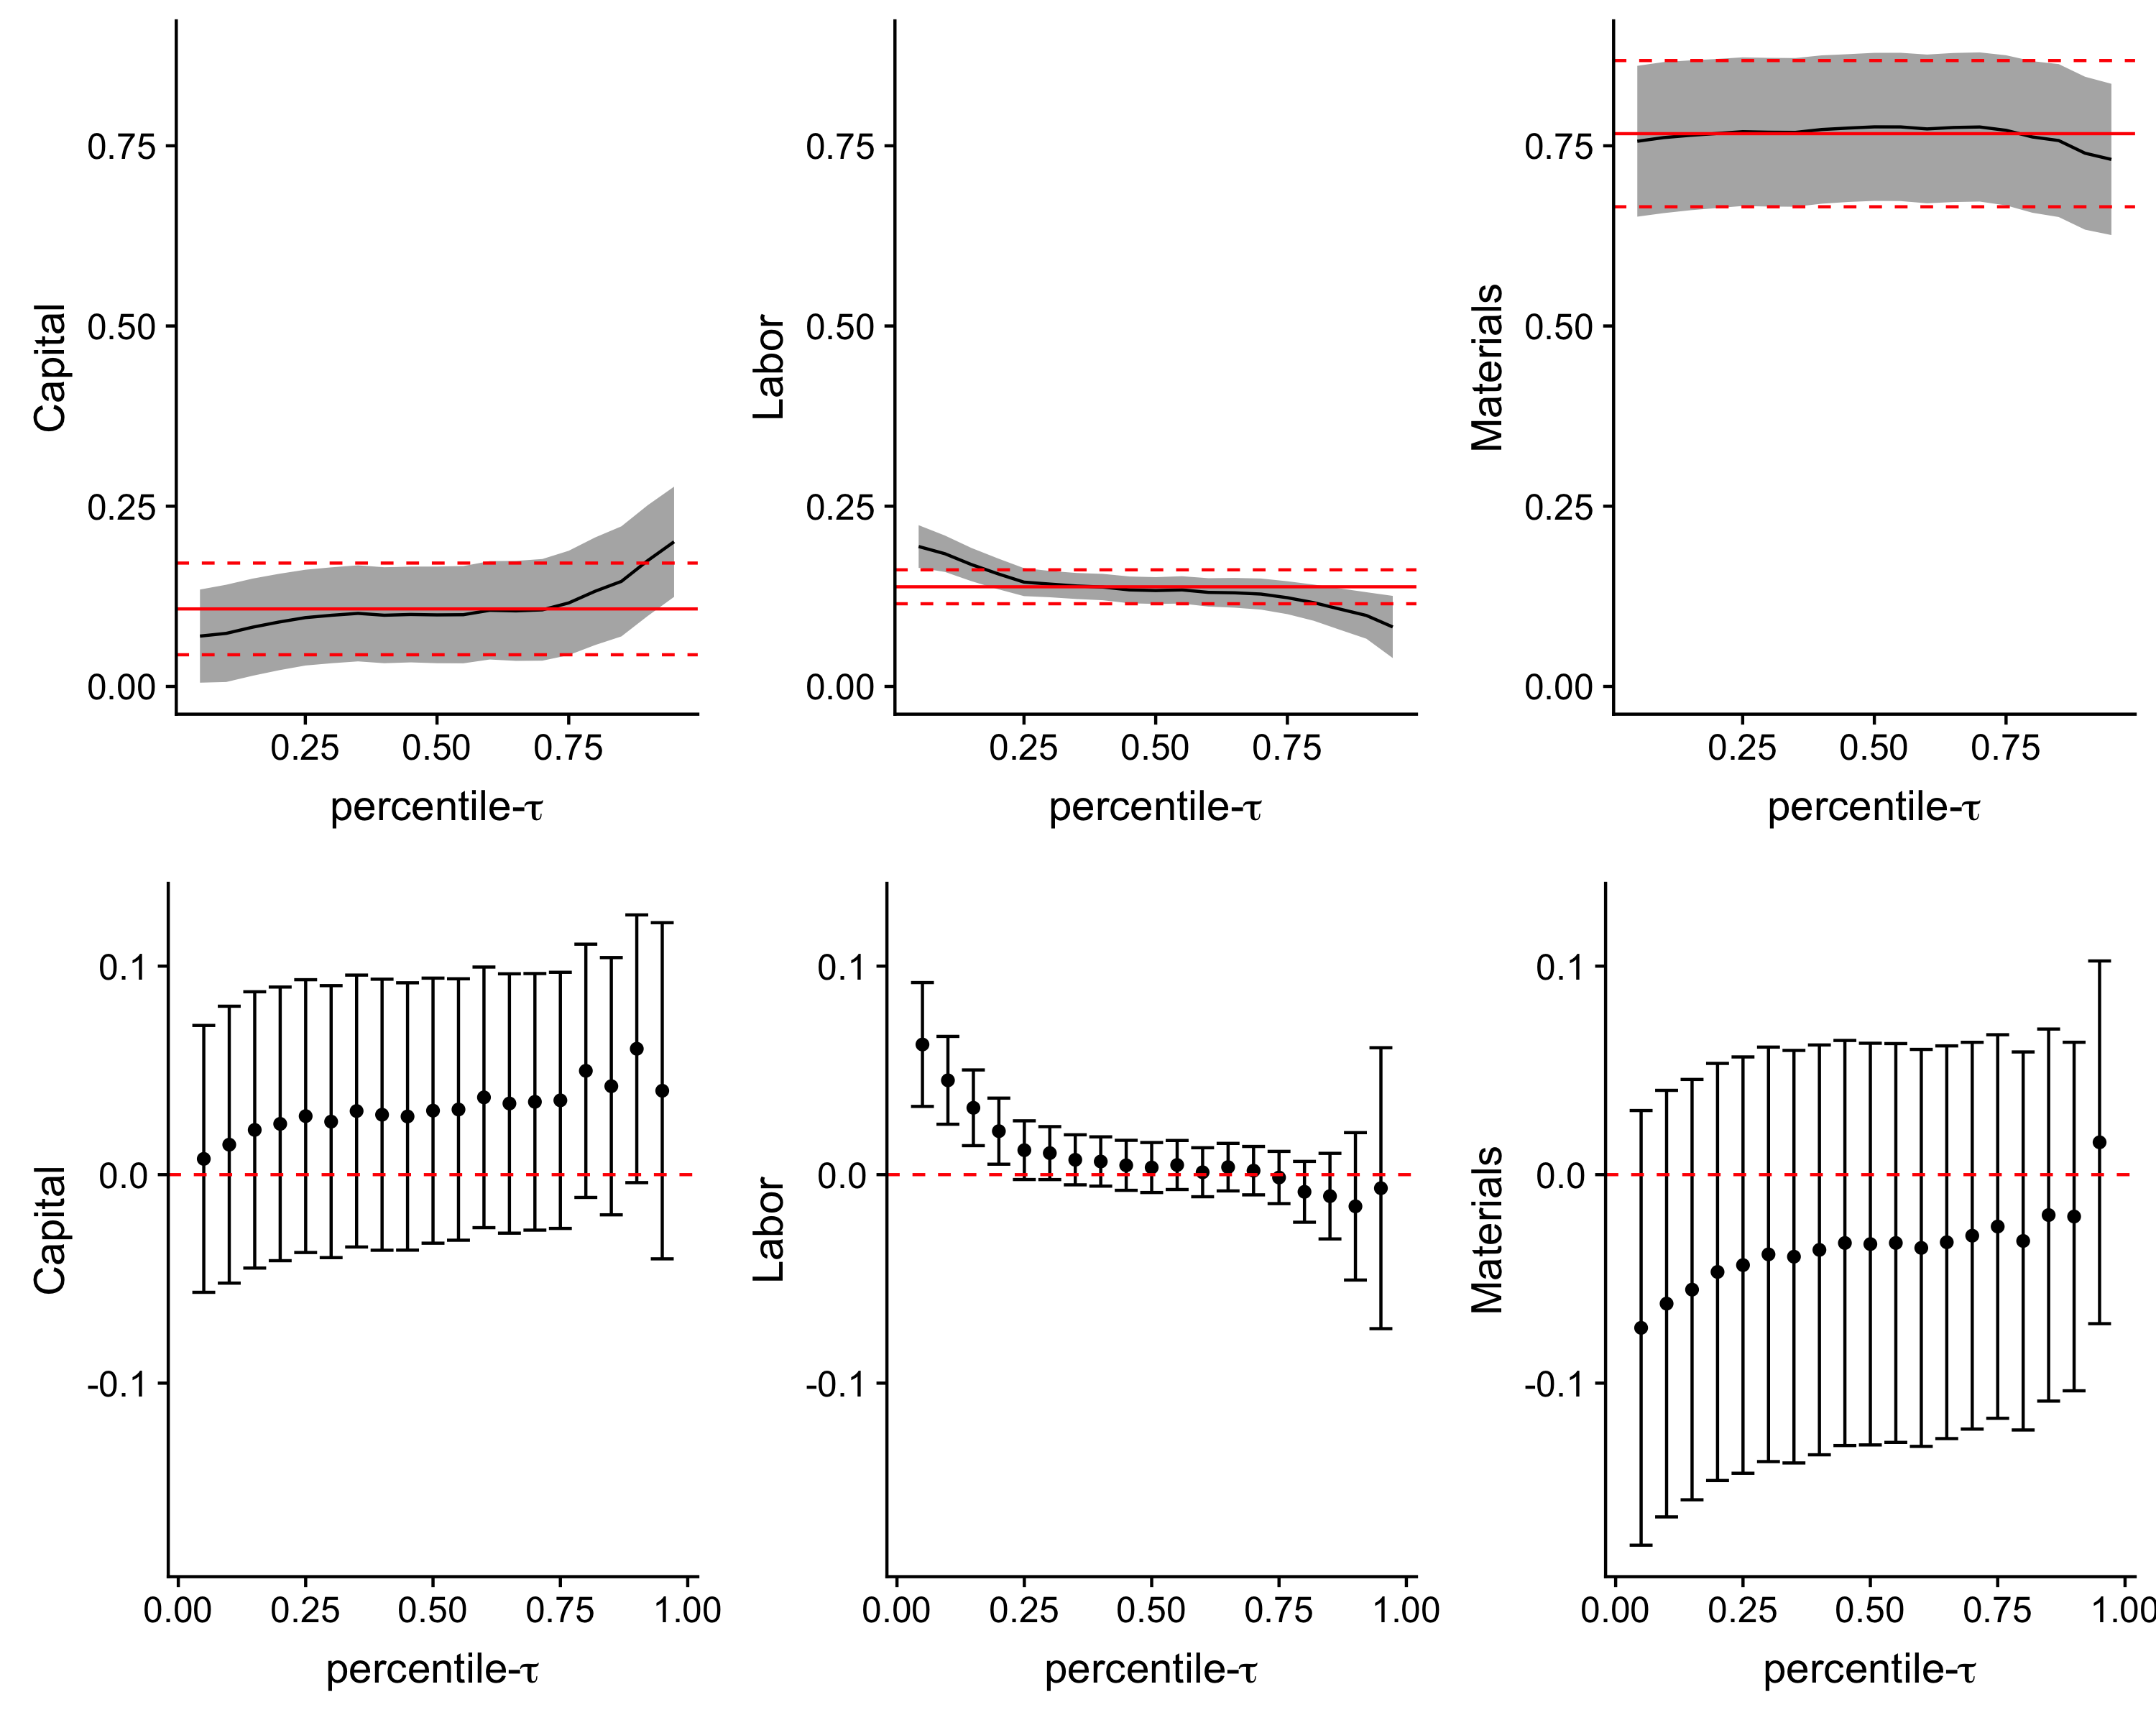
\includegraphics[width=8cm, height=8cm]{US/QLP_Coef_Plot_NAICS_31.png}
\caption*{\footnotesize $^{*}$Top row: Estimated values of production function coefficients and their point-wise 90\% confidence interval. Bottom row: Difference between DS and QR estimates that does not control for endogeneity and their 95\% confidence intervals.}
\label{fig:QLPUS31}
\end{figure}

\begin{figure}[H]
\centering
\caption{Estimated Coefficients of Capital and Labor for U.S.: NAICS 32}
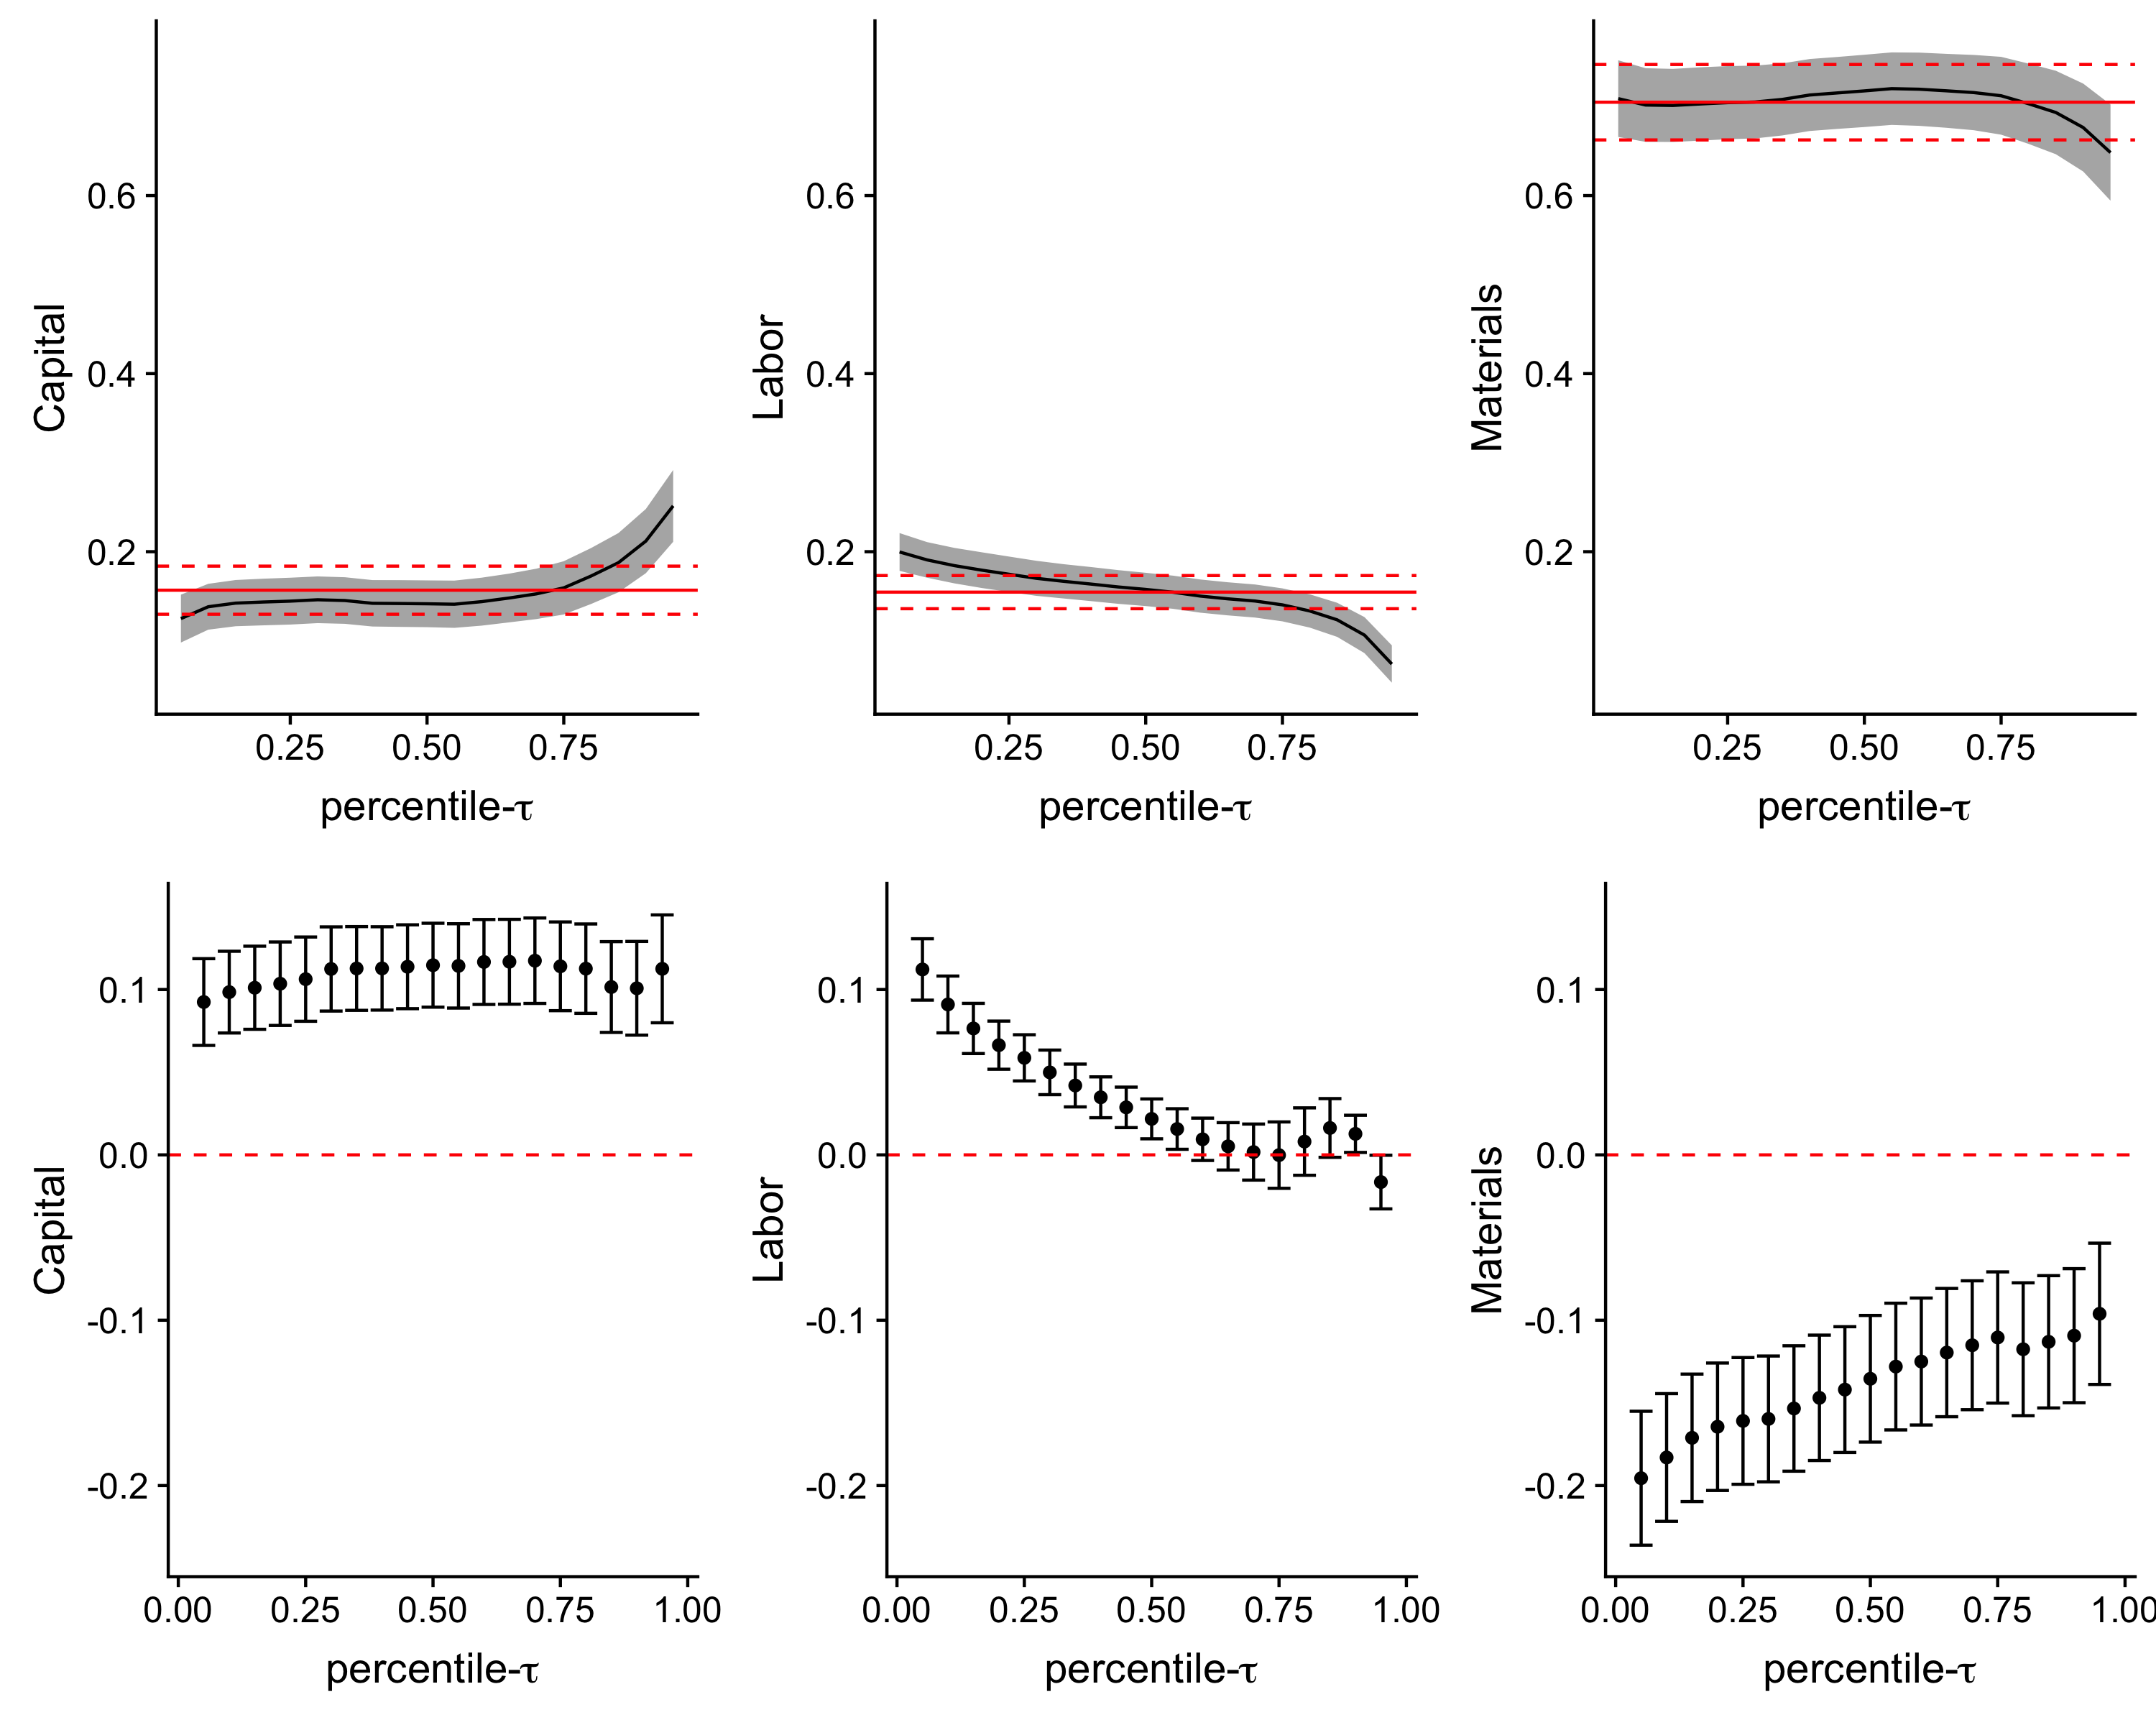
\includegraphics[width=8cm, height=8cm]{US/QLP_Coef_Plot_NAICS_32.png}
\caption*{\footnotesize $^{*}$Top row: Estimated values of production function coefficients and their point-wise 90\% confidence interval. Bottom row: Difference between DS and QR estimates that does not control for endogeneity and their 95\% confidence intervals.}
\label{fig:QLPUS32}
\end{figure}

\begin{figure}[H]
\centering
\caption{Estimated Coefficients of Capital and Labor for U.S.: NAICS 33}
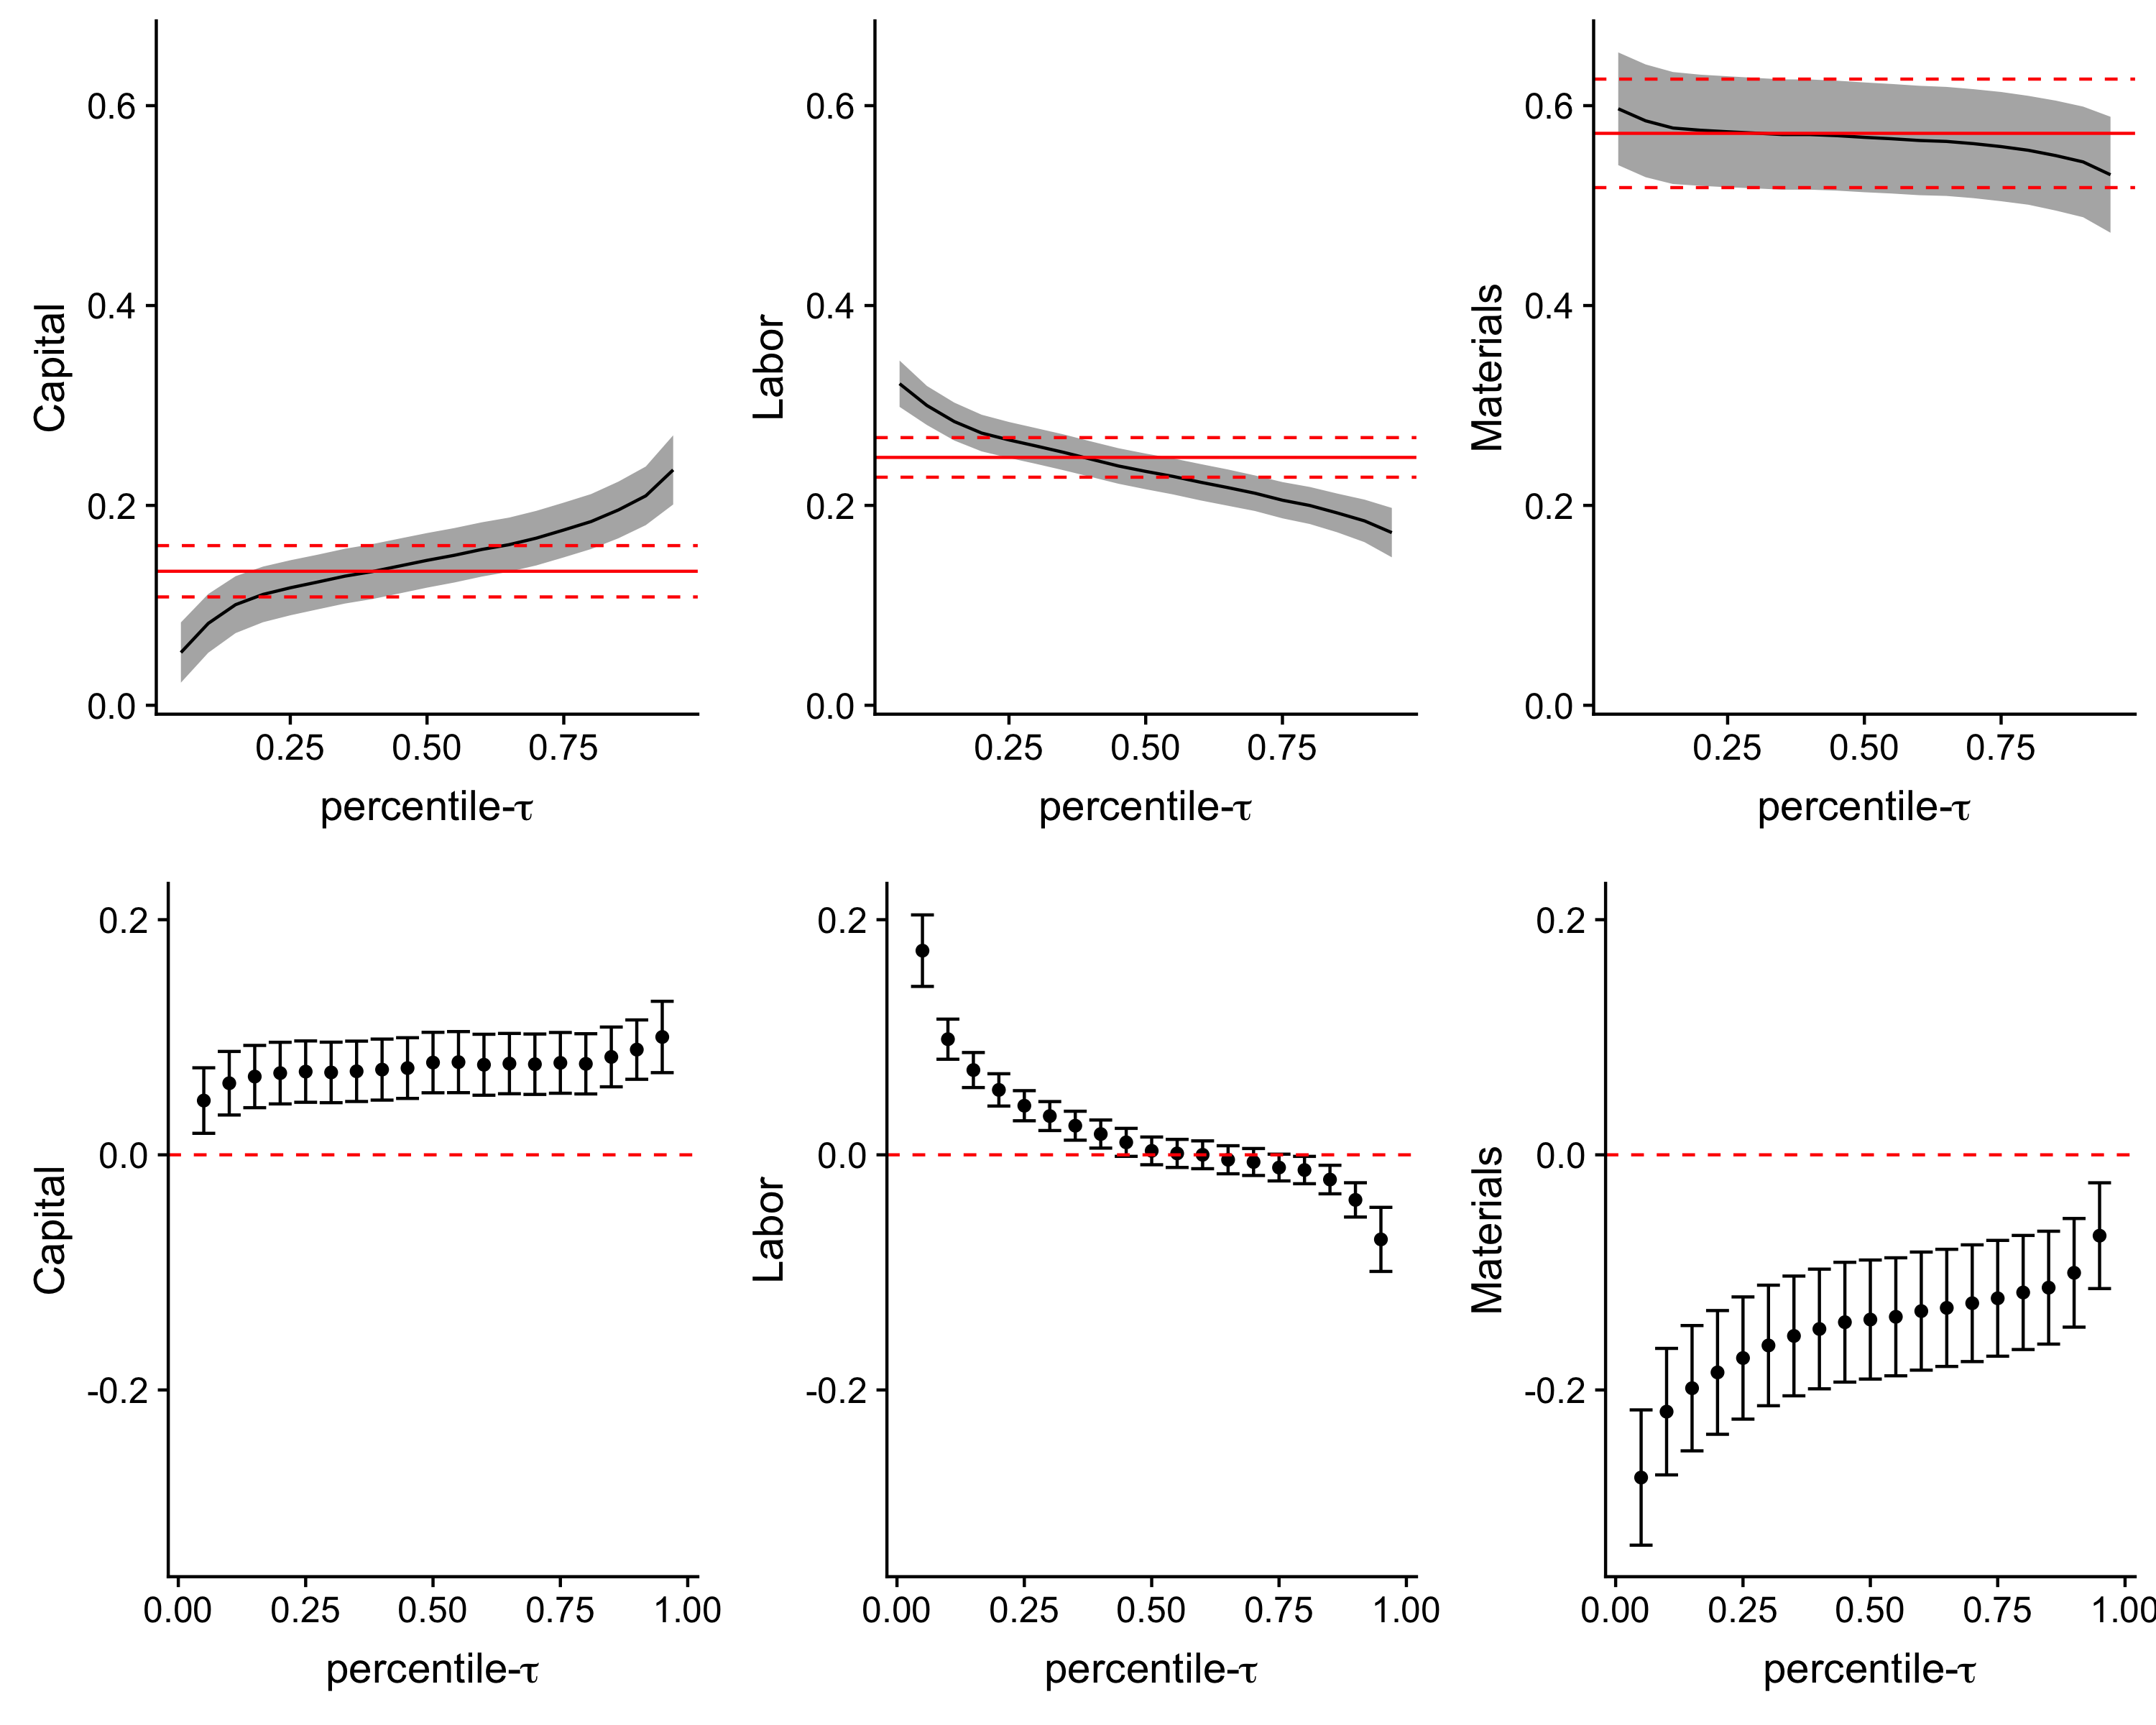
\includegraphics[width=8cm, height=8cm]{US/QLP_Coef_Plot_NAICS_33.png}
\caption*{\footnotesize $^{*}$Top row: Estimated values of production function coefficients and their point-wise 90\% confidence interval. Bottom row: Difference between DS and QR estimates that does not control for endogeneity and their 95\% confidence intervals.}
\label{fig:QLPUS33}
\end{figure}

\begin{figure}[H]
\centering
\caption{Estimated Coefficients of Capital and Labor U.S. Manufacturing Firms}
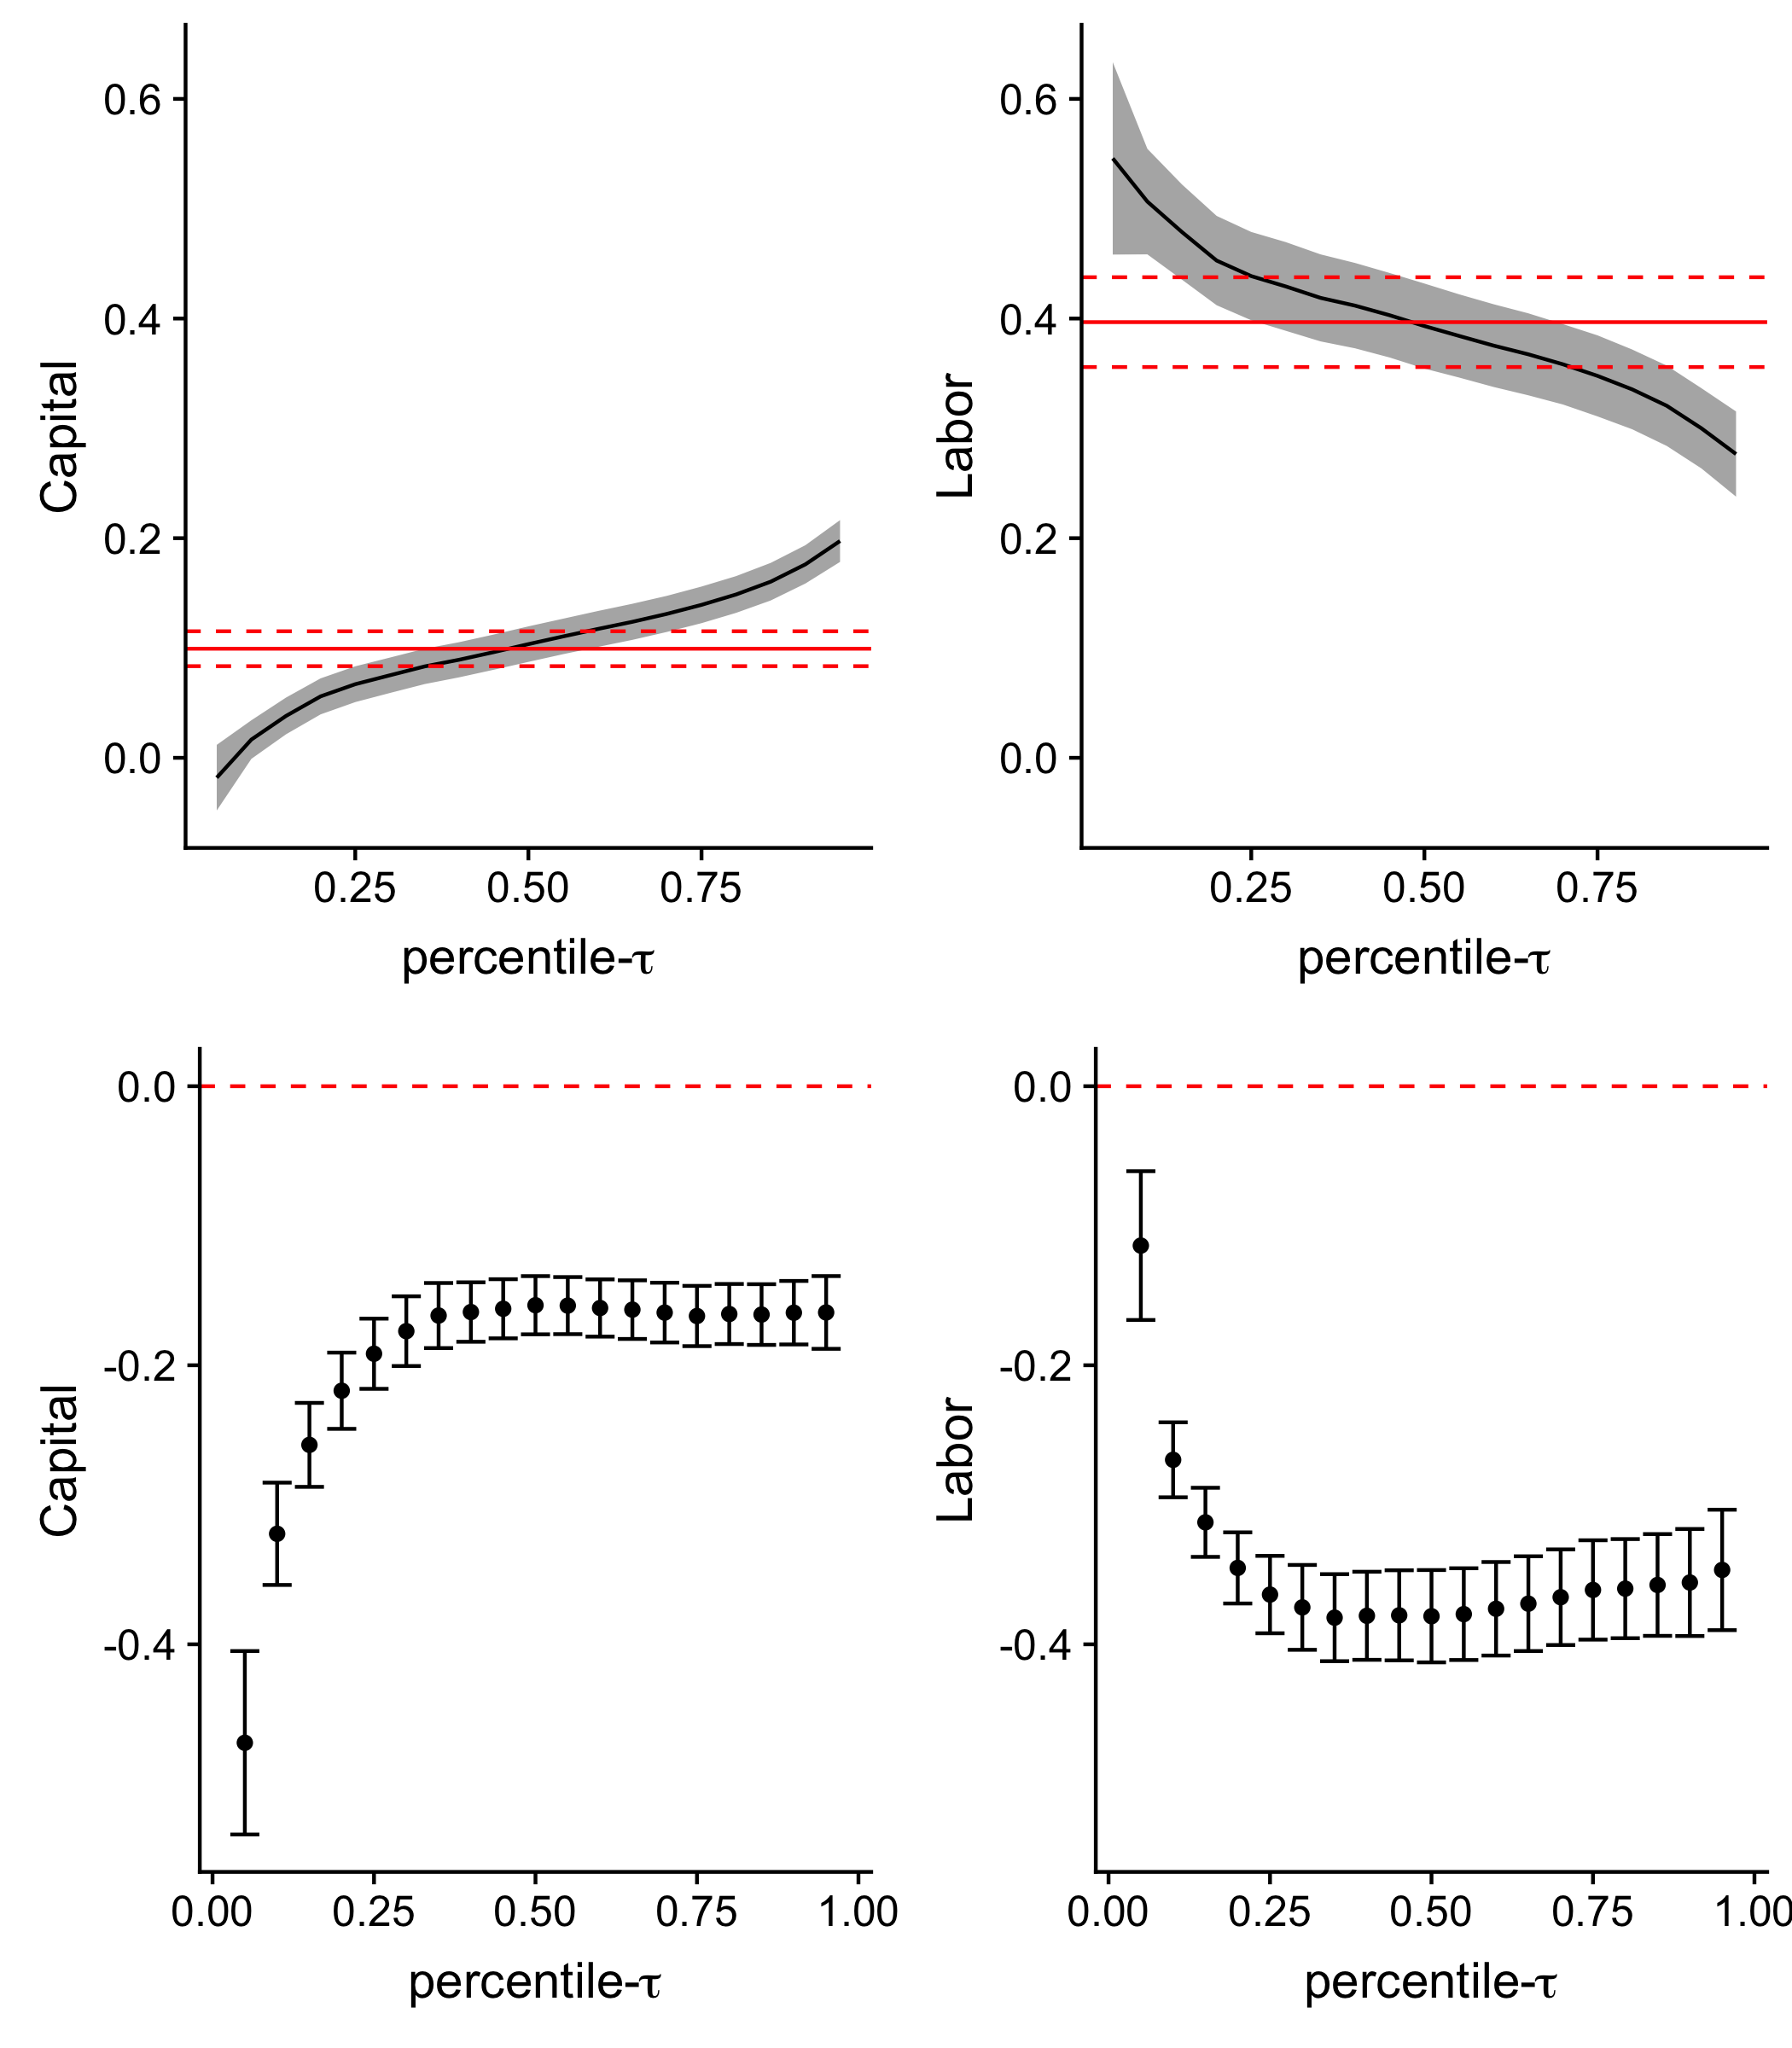
\includegraphics[width=8cm, height=8cm]{US/QLP_Coef_Plot_NAICS_All.png}
\caption*{\footnotesize $^{*}$Top row: Estimated values of production function coefficients and their point-wise 90\% confidence interval. Bottom row: Difference between DS and QR estimates that does not control for endogeneity and their 95\% confidence intervals.}
\label{fig:QLPUSall}
\end{figure}

\begin{figure}[H]
\centering
\caption{DS and LP Estimates of Log Total Factor Productivity}
\includegraphics[width=11cm]{US/QLP_TFP_Plot.png}
\caption*{\footnotesize $^{*}$Estimated distributions of TFP from the DS estimator for $\tau \in \{0.1, 0.5, 0.9\}$ and those from  the LP estimator.}
\label{fig:QLPUSTFP}
\end{figure}

\begin{figure}[H]
\centering
\caption{U.S. Productivity Over Time}
\includegraphics[width=11cm]{US/QLP_TFPgrowth_Plot.png}
\caption*{\footnotesize $^{*}$Estimated average productivity over time for the U.S. Base productivity in 1961 is set to 100.}
\label{fig:QLPUSTFPG}
\end{figure}

\begin{table}[H]
\centering
\caption{Productivity Differentials for U.S. Manufacturing Firms using DS}
\small
\begin{tabular}{cccccc}
  \hline\hline & & \multicolumn{2}{c}{R\&D}  & \multicolumn{2}{c}{Advertisements} \\ \cmidrule(lr){3-4} \cmidrule(lr){5-6}NAICS & $\tau$ & Coef. & s.e & Coef. & s.e \\ 
  \hline
31 & 0.10 & 0.011 & 0.0117 & 0.010 & 0.0140 \\ 
   & 0.25 & 0.011 & 0.0117 & 0.010 & 0.0141 \\ 
   & 0.50 & 0.017 & 0.0115 & 0.016 & 0.0137 \\ 
   & 0.90 & 0.012 & 0.0121 & 0.010 & 0.0140 \\ 
  32 & 0.10 & -0.008 & 0.0088 & -0.010 & 0.0093 \\ 
   & 0.25 & -0.004 & 0.0088 & -0.006 & 0.0093 \\ 
   & 0.50 & -0.001 & 0.0090 & -0.002 & 0.0095 \\ 
   & 0.90 & 0.011 & 0.0099 & 0.007 & 0.0102 \\ 
  33 & 0.10 & -0.001 & 0.0041 & -0.001 & 0.0037 \\ 
   & 0.25 & 0.007 & 0.0040 & 0.005 & 0.0037 \\ 
   & 0.50 & 0.015 & 0.0040 & 0.012 & 0.0037 \\ 
   & 0.90 & 0.023 & 0.0043 & 0.017 & 0.0039 \\ 
  All & 0.10 & -0.008 & 0.0039 & -0.012 & 0.0037 \\ 
   & 0.25 & -0.006 & 0.0037 & -0.010 & 0.0036 \\ 
   & 0.50 & -0.003 & 0.0037 & -0.007 & 0.0036 \\ 
   & 0.90 & 0.001 & 0.0040 & -0.006 & 0.0039 \\ 
   \hline
\end{tabular}
\caption*{\footnotesize $^{*}$Standard errors are obtained using bootstrap with 500 replications. Log(TFP) is regressed on log(R\&D) and log(Advertisements).}
\label{QLPUSTFPP}
\end{table}

\begin{table}[H]
\centering
\caption{Productivity Differentials for U.S. Manufacturing Firms using LP}
\small
\begin{tabular}{ccccc}
  \hline\hline & \multicolumn{2}{c}{R\&D}  & \multicolumn{2}{c}{Advertisements} \\ \cmidrule(lr){2-3} \cmidrule(lr){4-5}NAICS & Coef. & s.e & Coef. & s.e \\ 
  \hline
31 & 0.012 & 0.0110 & 0.010 & 0.0132 \\ 
  32 & -0.001 & 0.0090 & -0.003 & 0.0094 \\ 
  33 & 0.010 & 0.0040 & 0.008 & 0.0036 \\ 
  All & -0.005 & 0.0037 & -0.009 & 0.0036 \\ 
   \hline
\end{tabular}
\caption*{\footnotesize $^{*}$Standard errors are obtained using bootstrap with 500 replications. Log(TFP) is regressed on log(R\&D) and log(Advertisements).}
\label{LPUSTFPP}
\end{table}

\subsection{Chile}

\begin{table}[H]
\centering
\caption{Coefficient Estimates and Standard Errors for Chilean Manufacturing Plants}
\small
\begin{tabular}{cccccccccccc}
  \hline\hline & & \multicolumn{2}{c}{Capital}  & \multicolumn{2}{c}{Labor} & \multicolumn{2}{c}{Materials} & \multicolumn{2}{c}{Returns to Scale} & \multicolumn{2}{c}{Capital Intensity}\\ \cmidrule(lr){3-4} \cmidrule(lr){5-6} \cmidrule(lr){7-8} \cmidrule(lr){9-10} \cmidrule(lr){11-12}ISIC & $\tau$ & Coef. & s.e & Coef. & s.e & Coef. & s.e & Coef. & s.e & Coef. & s.e \\ 
  \hline
311 & 0.10 & 0.026 & 0.0058 & 0.109 & 0.0086 & 0.762 & 0.0106 & 0.898 & 0.0109 & 0.237 & 0.0610 \\ 
   & 0.25 & 0.045 & 0.0056 & 0.102 & 0.0065 & 0.761 & 0.0106 & 0.907 & 0.0106 & 0.437 & 0.0618 \\ 
   & 0.50 & 0.061 & 0.0059 & 0.118 & 0.0063 & 0.754 & 0.0105 & 0.934 & 0.0107 & 0.517 & 0.0592 \\ 
   & 0.90 & 0.081 & 0.0069 & 0.153 & 0.0111 & 0.756 & 0.0110 & 0.991 & 0.0118 & 0.528 & 0.0665 \\ 
  381 & 0.10 & 0.053 & 0.0137 & 0.326 & 0.0266 & 0.589 & 0.0183 & 0.968 & 0.0197 & 0.163 & 0.0502 \\ 
   & 0.25 & 0.084 & 0.0129 & 0.295 & 0.0195 & 0.594 & 0.0166 & 0.973 & 0.0161 & 0.285 & 0.0530 \\ 
   & 0.50 & 0.109 & 0.0131 & 0.274 & 0.0167 & 0.599 & 0.0158 & 0.982 & 0.0156 & 0.398 & 0.0611 \\ 
   & 0.90 & 0.132 & 0.0159 & 0.285 & 0.0273 & 0.615 & 0.0165 & 1.032 & 0.0213 & 0.462 & 0.0845 \\ 
  321 & 0.10 & 0.022 & 0.0121 & 0.272 & 0.0224 & 0.620 & 0.0169 & 0.914 & 0.0178 & 0.082 & 0.0475 \\ 
   & 0.25 & 0.048 & 0.0120 & 0.253 & 0.0168 & 0.621 & 0.0152 & 0.923 & 0.0154 & 0.191 & 0.0532 \\ 
   & 0.50 & 0.072 & 0.0121 & 0.232 & 0.0152 & 0.625 & 0.0144 & 0.929 & 0.0150 & 0.310 & 0.0646 \\ 
   & 0.90 & 0.108 & 0.0131 & 0.202 & 0.0204 & 0.639 & 0.0150 & 0.949 & 0.0178 & 0.536 & 0.1000 \\ 
  All & 0.10 & 0.038 & 0.0043 & 0.187 & 0.0070 & 0.672 & 0.0062 & 0.898 & 0.0063 & 0.205 & 0.0255 \\ 
   & 0.25 & 0.074 & 0.0043 & 0.165 & 0.0062 & 0.667 & 0.0061 & 0.906 & 0.0060 & 0.450 & 0.0338 \\ 
   & 0.50 & 0.104 & 0.0043 & 0.155 & 0.0057 & 0.664 & 0.0059 & 0.923 & 0.0057 & 0.670 & 0.0409 \\ 
   & 0.90 & 0.148 & 0.0055 & 0.174 & 0.0100 & 0.663 & 0.0064 & 0.984 & 0.0071 & 0.852 & 0.0708 \\ 
   \hline
\end{tabular}
\caption*{\footnotesize $^{*}$ Standard errors are obtained using bootstrap with 500 replications. The first stage uses estimates from LP.}
\label{CHLQLP}
\end{table}

\begin{table}[H]
\centering
\caption{LP Coefficient Estimates and Standard Errors for Chilean Manufacturing Plants}
\small
\begin{tabular}{ccccccccccc}
  \hline\hline & \multicolumn{2}{c}{Capital} & \multicolumn{2}{c}{Labor} & \multicolumn{2}{c}{Materials} & \multicolumn{2}{c}{Returns to Scale} & \multicolumn{2}{c}{Capital Intensity}\\ \cmidrule(lr){2-3} \cmidrule(lr){4-5} \cmidrule(lr){6-7} \cmidrule(lr){8-9} \cmidrule(lr){10-11}ISIC & Coef. & s.e & Coef. & s.e & Coef. & s.e & Coef. & s.e & Coef. & s.e \\ 
  \hline
311 & 0.057 & 0.0055 & 0.133 & 0.0069 & 0.755 & 0.0105 & 0.945 & 0.0105 & 0.427 & 0.0496 \\ 
  381 & 0.093 & 0.0130 & 0.288 & 0.0187 & 0.607 & 0.0154 & 0.988 & 0.0157 & 0.325 & 0.0574 \\ 
  321 & 0.067 & 0.0106 & 0.234 & 0.0146 & 0.629 & 0.0140 & 0.930 & 0.0150 & 0.286 & 0.0539 \\ 
  All & 0.095 & 0.0039 & 0.171 & 0.0062 & 0.668 & 0.0059 & 0.934 & 0.0055 & 0.554 & 0.0343 \\ 
   \hline
\end{tabular}
\caption*{\footnotesize $^{*}$Standard errors are obtained using bootstrap with 500 replications.}
\label{CHLLP}
\end{table}

\begin{figure}[H]
\centering
\caption{Estimated Coefficients of Capital and Labor for Chile: ISIC 311}
\includegraphics[width=8cm, height=8cm]{Chile/QLP_Coef_Plot_ISIC_311.png}
\caption*{\footnotesize $^{*}$Top row: Estimated values of production function coefficients and their point-wise 90\% confidence interval. Bottom row: Difference between DS and QR estimates that does not control for endogeneity and their 95\% confidence intervals.}
\label{fig:QLPCHL311}
\end{figure}

\begin{figure}[H]
\centering
\caption{Estimated Coefficients of Capital and Labor for Chile: ISIC 381}
\includegraphics[width=8cm, height=8cm]{Chile//QLP_Coef_Plot_ISIC_381.png}
\caption*{\footnotesize $^{*}$Top row: Estimated values of production function coefficients and their point-wise 90\% confidence interval. Bottom row: Difference between DS and QR estimates that does not control for endogeneity and their 95\% confidence intervals.}
\label{fig:QLPCHL381}
\end{figure}

\begin{figure}[H]
\centering
\caption{Estimated Coefficients of Capital and Labor for Chile: ISIC 321}
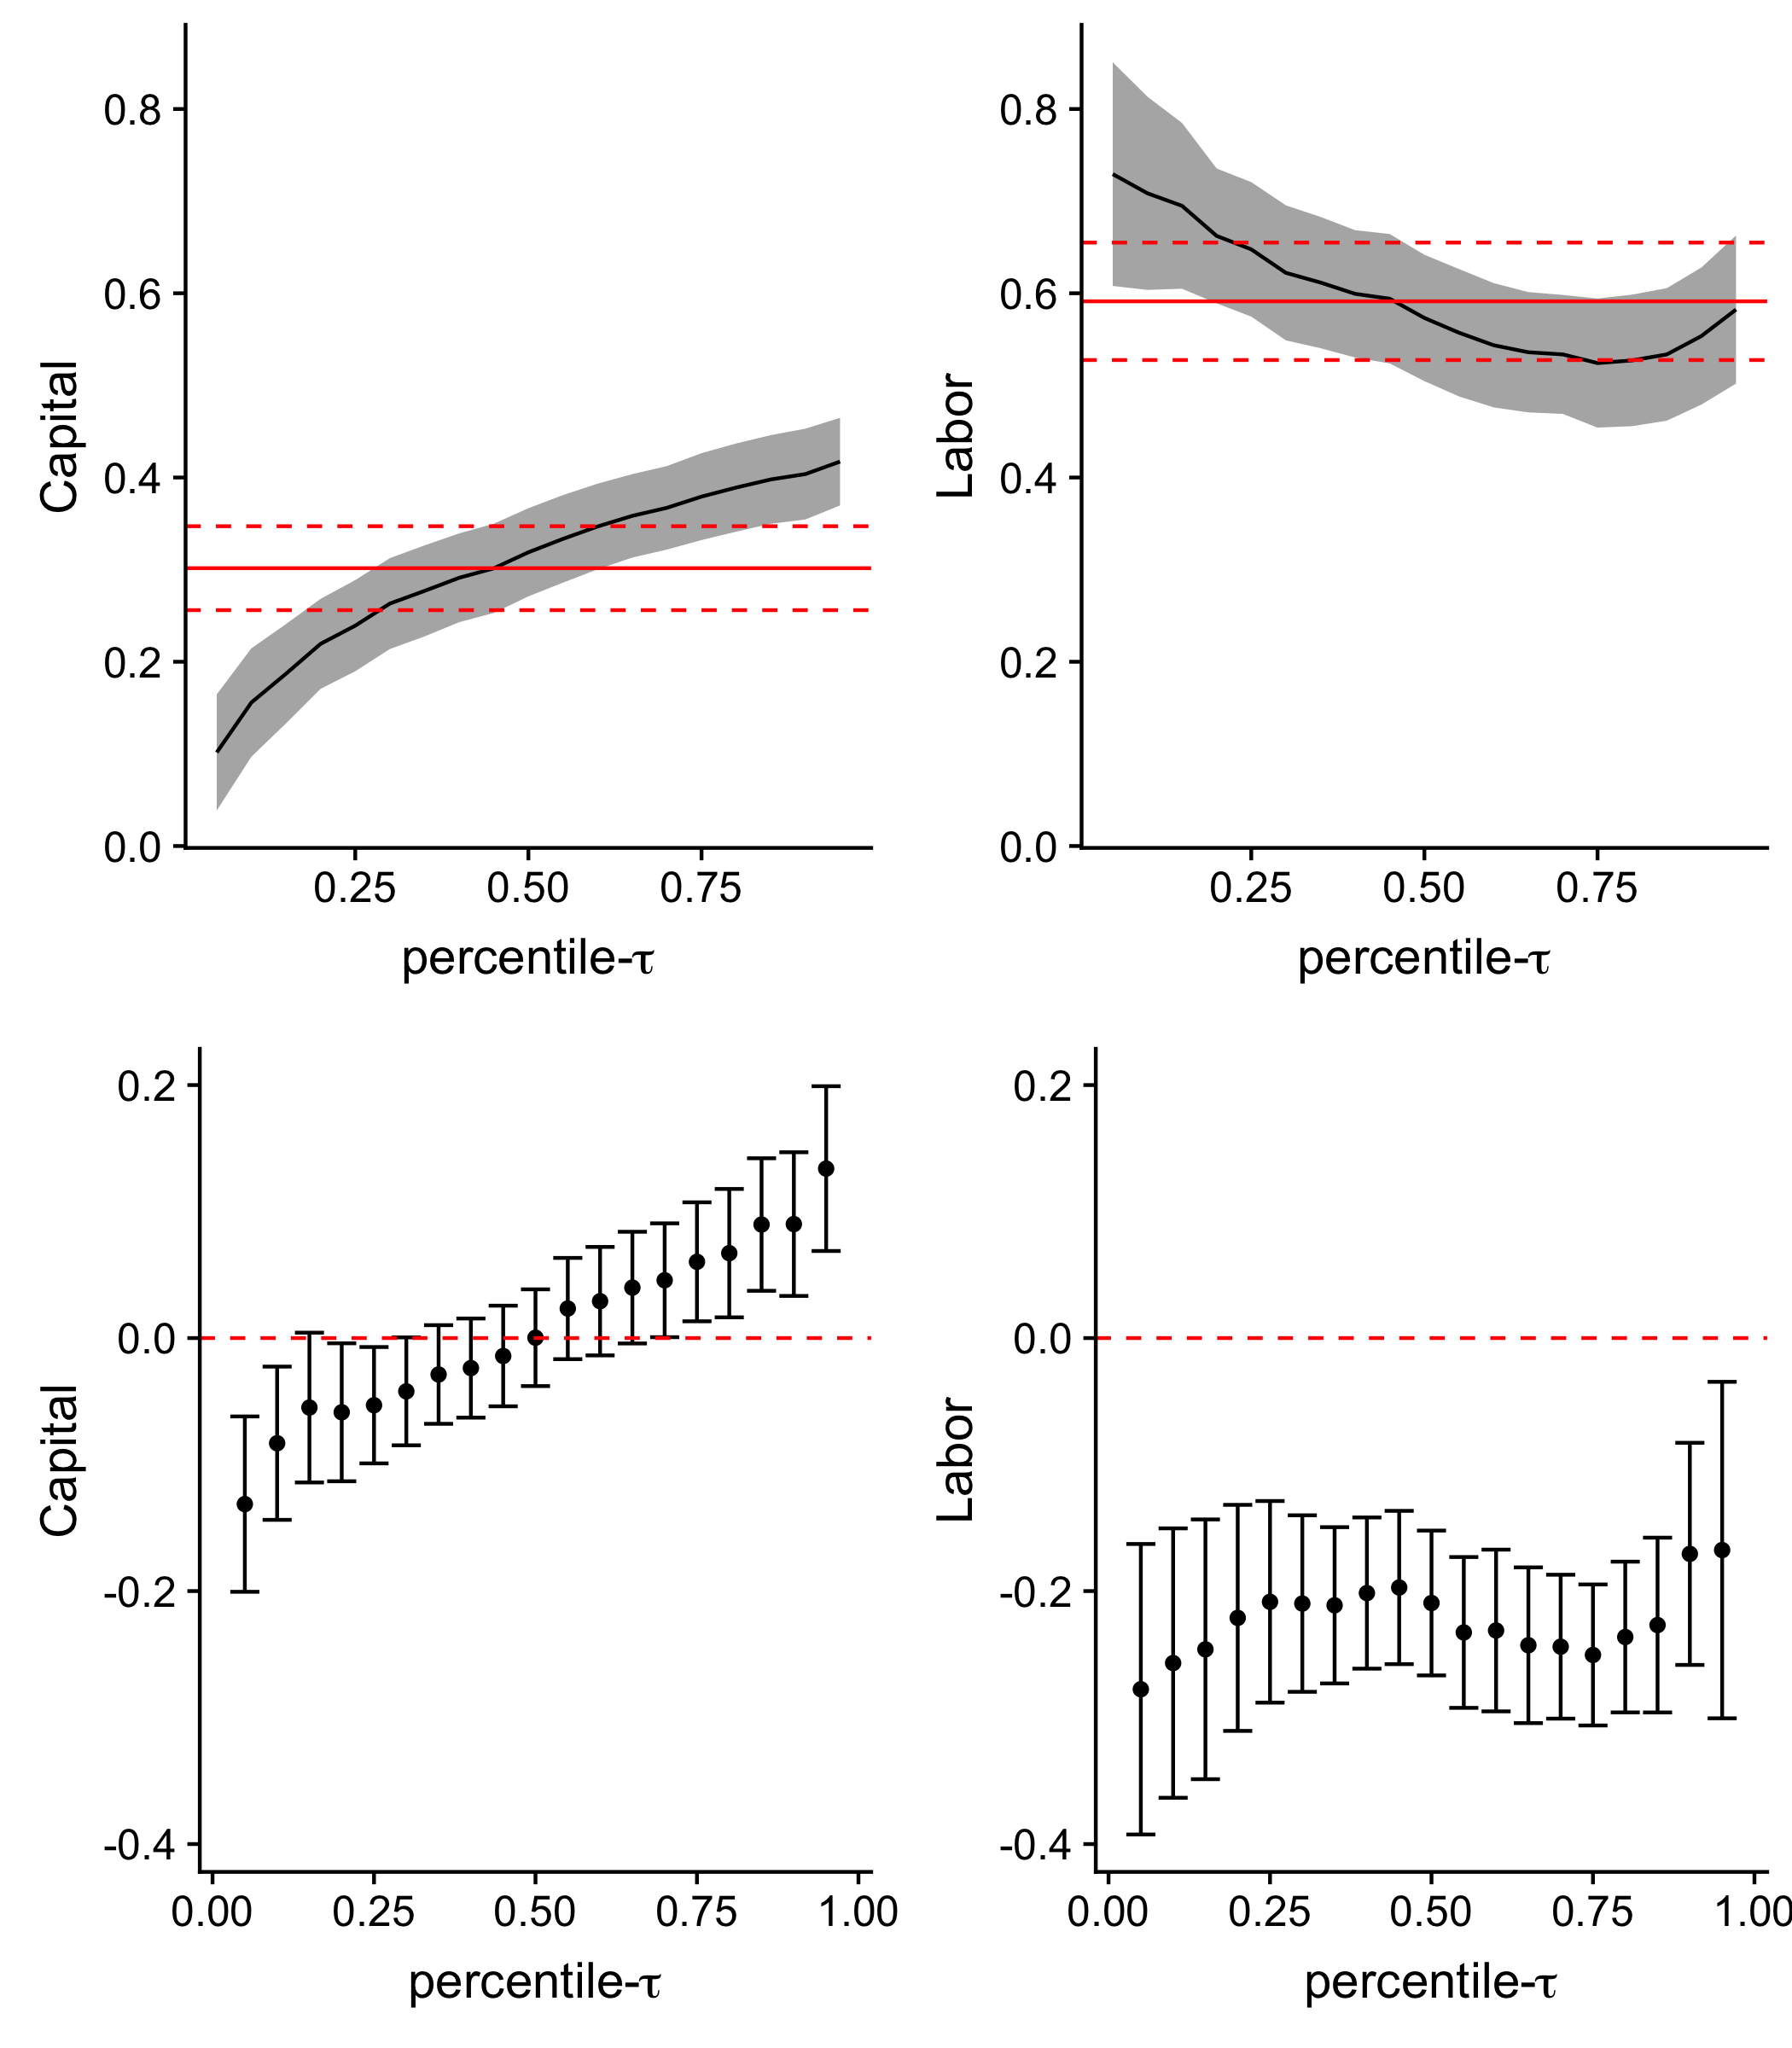
\includegraphics[width=8cm, height=8cm]{Chile//QLP_Coef_Plot_ISIC_321.png}
\caption*{\footnotesize $^{*}$Top row: Estimated values of production function coefficients and their point-wise 90\% confidence interval. Bottom row: Difference between DS and QR estimates that does not control for endogeneity and their 95\% confidence intervals.}
\label{fig:QLPCHL321}
\end{figure}

\begin{figure}[H]
\centering
\caption{Estimated Coefficients of Capital and Labor for Chilean Manufacturing Plants}
\includegraphics[width=8cm, height=8cm]{Chile//QLP_Coef_Plot_ISIC_All.png}
\caption*{\footnotesize $^{*}$Top row: Estimated values of production function coefficients and their point-wise 90\% confidence interval. Bottom row: Difference between DS and QR estimates that does not control for endogeneity and their 95\% confidence intervals.}
\label{fig:QLPCHLall}
\end{figure}

\begin{figure}[H]
\centering
\caption{DS and LP Estimates of Log Total Factor Productivity}
\includegraphics[width=11cm]{Chile/QLP_TFP_Plot.png}
\caption*{\footnotesize $^{*}$Estimated distributions of TFP from the DS estimator for $\tau \in \{0.1, 0.5, 0.9\}$ and those from  the LP estimator.}
\label{fig:QLPCHLTFP}
\end{figure}

\begin{figure}[H]
\centering
\caption{Chile Productivity Over Time}
\includegraphics[width=11cm]{Chile/QLP_TFPgrowth_Plot.png}
\caption*{\footnotesize $^{*}$Estimated average productivity over time for Chile. Productivity in the base year is set to 100.}
\label{fig:QLPCHLTFPG}
\end{figure}

\begin{table}[H]
\centering
\caption{Productivity Differentials for Chilean Manufacturing Plants using DS}
\small
\begin{tabular}{cccccccc}
  \hline\hline & & \multicolumn{2}{c}{Exports}  & \multicolumn{2}{c}{Imports} & \multicolumn{2}{c}{Advertisements} \\ \cmidrule(lr){3-4} \cmidrule(lr){5-6} \cmidrule(lr){7-8}ISIC & $\tau$ & Coef. & s.e & Coef. & s.e & Coef. & s.e \\ 
  \hline
311 & 0.10 & 0.026 & 0.0110 & 0.039 & 0.0122 & 0.019 & 0.0087 \\ 
   & 0.25 & 0.022 & 0.0108 & 0.037 & 0.0120 & 0.017 & 0.0087 \\ 
   & 0.50 & 0.018 & 0.0107 & 0.028 & 0.0116 & 0.012 & 0.0087 \\ 
   & 0.90 & 0.012 & 0.0111 & 0.009 & 0.0120 & 0.002 & 0.0088 \\ 
  381 & 0.10 & 0.024 & 0.0125 & 0.049 & 0.0176 & 0.037 & 0.0154 \\ 
   & 0.25 & 0.016 & 0.0123 & 0.037 & 0.0179 & 0.030 & 0.0149 \\ 
   & 0.50 & 0.008 & 0.0125 & 0.026 & 0.0185 & 0.024 & 0.0149 \\ 
   & 0.90 & -0.011 & 0.0136 & -0.003 & 0.0196 & 0.006 & 0.0165 \\ 
  321 & 0.10 & 0.022 & 0.0111 & 0.031 & 0.0145 & 0.043 & 0.0133 \\ 
   & 0.25 & 0.019 & 0.0107 & 0.027 & 0.0140 & 0.040 & 0.0122 \\ 
   & 0.50 & 0.018 & 0.0107 & 0.023 & 0.0142 & 0.038 & 0.0122 \\ 
   & 0.90 & 0.012 & 0.0112 & 0.012 & 0.0152 & 0.031 & 0.0130 \\ 
  All & 0.10 & 0.038 & 0.0047 & 0.061 & 0.0070 & 0.053 & 0.0055 \\ 
   & 0.25 & 0.031 & 0.0046 & 0.054 & 0.0069 & 0.051 & 0.0053 \\ 
   & 0.50 & 0.023 & 0.0046 & 0.045 & 0.0068 & 0.046 & 0.0052 \\ 
   & 0.90 & 0.002 & 0.0046 & 0.017 & 0.0069 & 0.030 & 0.0053 \\ 
   \hline
\end{tabular}
\caption*{\footnotesize $^{*}$Standard errors are obtained using bootstrap with 500 replications. Log(TFP) is regressed on log(Exports), log(Imports), and log(Advertisements).}
\label{QLPCHLTFPP}
\end{table}

\begin{table}[H]
\centering
\caption{Productivity Differentials for Chilean Manufacturing Plants using LP}
\small
\begin{tabular}{ccccccc}
  \hline\hline & \multicolumn{2}{c}{Exports}  & \multicolumn{2}{c}{Imports} & \multicolumn{2}{c}{Advertisements} \\ \cmidrule(lr){2-3} \cmidrule(lr){4-5} \cmidrule(lr){6-7}ISIC & Coef. & s.e & Coef. & s.e & Coef. & s.e \\ 
  \hline
311 & 0.018 & 0.0108 & 0.024 & 0.0117 & 0.010 & 0.0086 \\ 
  381 & 0.008 & 0.0124 & 0.026 & 0.0182 & 0.023 & 0.0149 \\ 
  321 & 0.017 & 0.0106 & 0.022 & 0.0139 & 0.037 & 0.0122 \\ 
  All & 0.021 & 0.0046 & 0.042 & 0.0068 & 0.043 & 0.0052 \\ 
   \hline
\end{tabular}
\caption*{\footnotesize $^{*}$Standard errors are obtained using bootstrap with 500 replications. Log(TFP) is regressed on log(Exports), log(Imports), and log(Advertisements).}
\label{LPCHLTFPP}
\end{table}

\subsection{Colombia}

\begin{table}[H]
\centering
\caption{Coefficient Estimates and Standard Errors for Colombian Manufacturing Plants}
\small
\begin{tabular}{cccccccccccc}
  \hline\hline & & \multicolumn{2}{c}{Capital}  & \multicolumn{2}{c}{Labor} & \multicolumn{2}{c}{Materials} & \multicolumn{2}{c}{Returns to Scale} & \multicolumn{2}{c}{Capital Intensity}\\ \cmidrule(lr){3-4} \cmidrule(lr){5-6} \cmidrule(lr){7-8} \cmidrule(lr){9-10} \cmidrule(lr){11-12}ISIC & $\tau$ & Coef. & s.e & Coef. & s.e & Coef. & s.e & Coef. & s.e & Coef. & s.e \\ 
  \hline
311 & 0.10 & 0.049 & 0.0139 & 0.199 & 0.0174 & 0.648 & 0.0170 & 0.896 & 0.0167 & 0.244 & 0.0799 \\ 
   & 0.25 & 0.083 & 0.0137 & 0.179 & 0.0103 & 0.642 & 0.0169 & 0.904 & 0.0142 & 0.466 & 0.0856 \\ 
   & 0.50 & 0.110 & 0.0143 & 0.155 & 0.0078 & 0.642 & 0.0173 & 0.906 & 0.0139 & 0.707 & 0.1035 \\ 
   & 0.90 & 0.198 & 0.0166 & 0.144 & 0.0151 & 0.612 & 0.0188 & 0.954 & 0.0156 & 1.373 & 0.1989 \\ 
  322 & 0.10 & 0.112 & 0.0157 & 0.394 & 0.0198 & 0.410 & 0.0165 & 0.916 & 0.0233 & 0.285 & 0.0451 \\ 
   & 0.25 & 0.157 & 0.0155 & 0.353 & 0.0162 & 0.408 & 0.0161 & 0.917 & 0.0218 & 0.444 & 0.0522 \\ 
   & 0.50 & 0.198 & 0.0167 & 0.302 & 0.0155 & 0.412 & 0.0163 & 0.912 & 0.0216 & 0.655 & 0.0705 \\ 
   & 0.90 & 0.270 & 0.0231 & 0.256 & 0.0243 & 0.415 & 0.0185 & 0.942 & 0.0228 & 1.053 & 0.1670 \\ 
  381 & 0.10 & 0.070 & 0.0251 & 0.339 & 0.0244 & 0.378 & 0.0221 & 0.787 & 0.0320 & 0.206 & 0.0811 \\ 
   & 0.25 & 0.113 & 0.0249 & 0.291 & 0.0176 & 0.380 & 0.0208 & 0.784 & 0.0308 & 0.388 & 0.0922 \\ 
   & 0.50 & 0.153 & 0.0249 & 0.254 & 0.0170 & 0.377 & 0.0203 & 0.785 & 0.0312 & 0.602 & 0.1137 \\ 
   & 0.90 & 0.261 & 0.0287 & 0.218 & 0.0294 & 0.348 & 0.0239 & 0.827 & 0.0333 & 1.197 & 0.2541 \\ 
  All & 0.10 & 0.072 & 0.0060 & 0.309 & 0.0070 & 0.468 & 0.0070 & 0.849 & 0.0078 & 0.234 & 0.0210 \\ 
   & 0.25 & 0.110 & 0.0060 & 0.280 & 0.0058 & 0.468 & 0.0066 & 0.859 & 0.0075 & 0.393 & 0.0247 \\ 
   & 0.50 & 0.148 & 0.0061 & 0.256 & 0.0048 & 0.466 & 0.0066 & 0.870 & 0.0071 & 0.578 & 0.0285 \\ 
   & 0.90 & 0.238 & 0.0072 & 0.257 & 0.0090 & 0.442 & 0.0073 & 0.937 & 0.0082 & 0.927 & 0.0492 \\ 
   \hline
\end{tabular}
\caption*{\footnotesize $^{*}$ Standard errors are obtained using bootstrap with 500 replications. The first stage uses estimates from LP.}
\label{COLestLP}
\end{table}

\begin{table}[H]
\centering
\caption{LP Coefficient Estimates and Standard Errors for Colombian Manufacturing Plants}
\small
\begin{tabular}{ccccccccccc}
  \hline\hline & \multicolumn{2}{c}{Capital} & \multicolumn{2}{c}{Labor} & \multicolumn{2}{c}{Materials} & \multicolumn{2}{c}{Returns to Scale} & \multicolumn{2}{c}{Capital Intensity}\\ \cmidrule(lr){2-3} \cmidrule(lr){4-5} \cmidrule(lr){6-7} \cmidrule(lr){8-9} \cmidrule(lr){10-11}ISIC & Coef. & s.e & Coef. & s.e & Coef. & s.e & Coef. & s.e & Coef. & s.e \\ 
  \hline
311 & 0.121 & 0.0135 & 0.166 & 0.0109 & 0.633 & 0.0178 & 0.919 & 0.0142 & 0.730 & 0.0960 \\ 
  322 & 0.189 & 0.0166 & 0.305 & 0.0175 & 0.420 & 0.0162 & 0.914 & 0.0219 & 0.621 & 0.0717 \\ 
  381 & 0.162 & 0.0256 & 0.244 & 0.0212 & 0.378 & 0.0205 & 0.784 & 0.0308 & 0.663 & 0.1385 \\ 
  All & 0.153 & 0.0059 & 0.266 & 0.0069 & 0.461 & 0.0068 & 0.881 & 0.0077 & 0.576 & 0.0294 \\ 
   \hline
\end{tabular}
\caption*{\footnotesize $^{*}$Standard errors are obtained using bootstrap with 500 replications.}
\label{COLLPcoef}
\end{table}

\begin{figure}[H]
\centering
\caption{Estimated Coefficients of Capital and Labor for Colombia: ISIC 311}
\includegraphics[width=8cm, height=8cm]{Colombia/QLP_Coef_Plot_ISIC_311.png}
\caption*{\footnotesize $^{*}$Top row: Estimated values of production function coefficients and their point-wise 90\% confidence interval. Bottom row: Difference between DS and QR estimates that does not control for endogeneity and their 95\% confidence intervals.}
\label{fig:LPCOL311}
\end{figure}

\begin{figure}[H]
\centering
\caption{Estimated Coefficients of Capital and Labor for Colombia: ISIC 321}
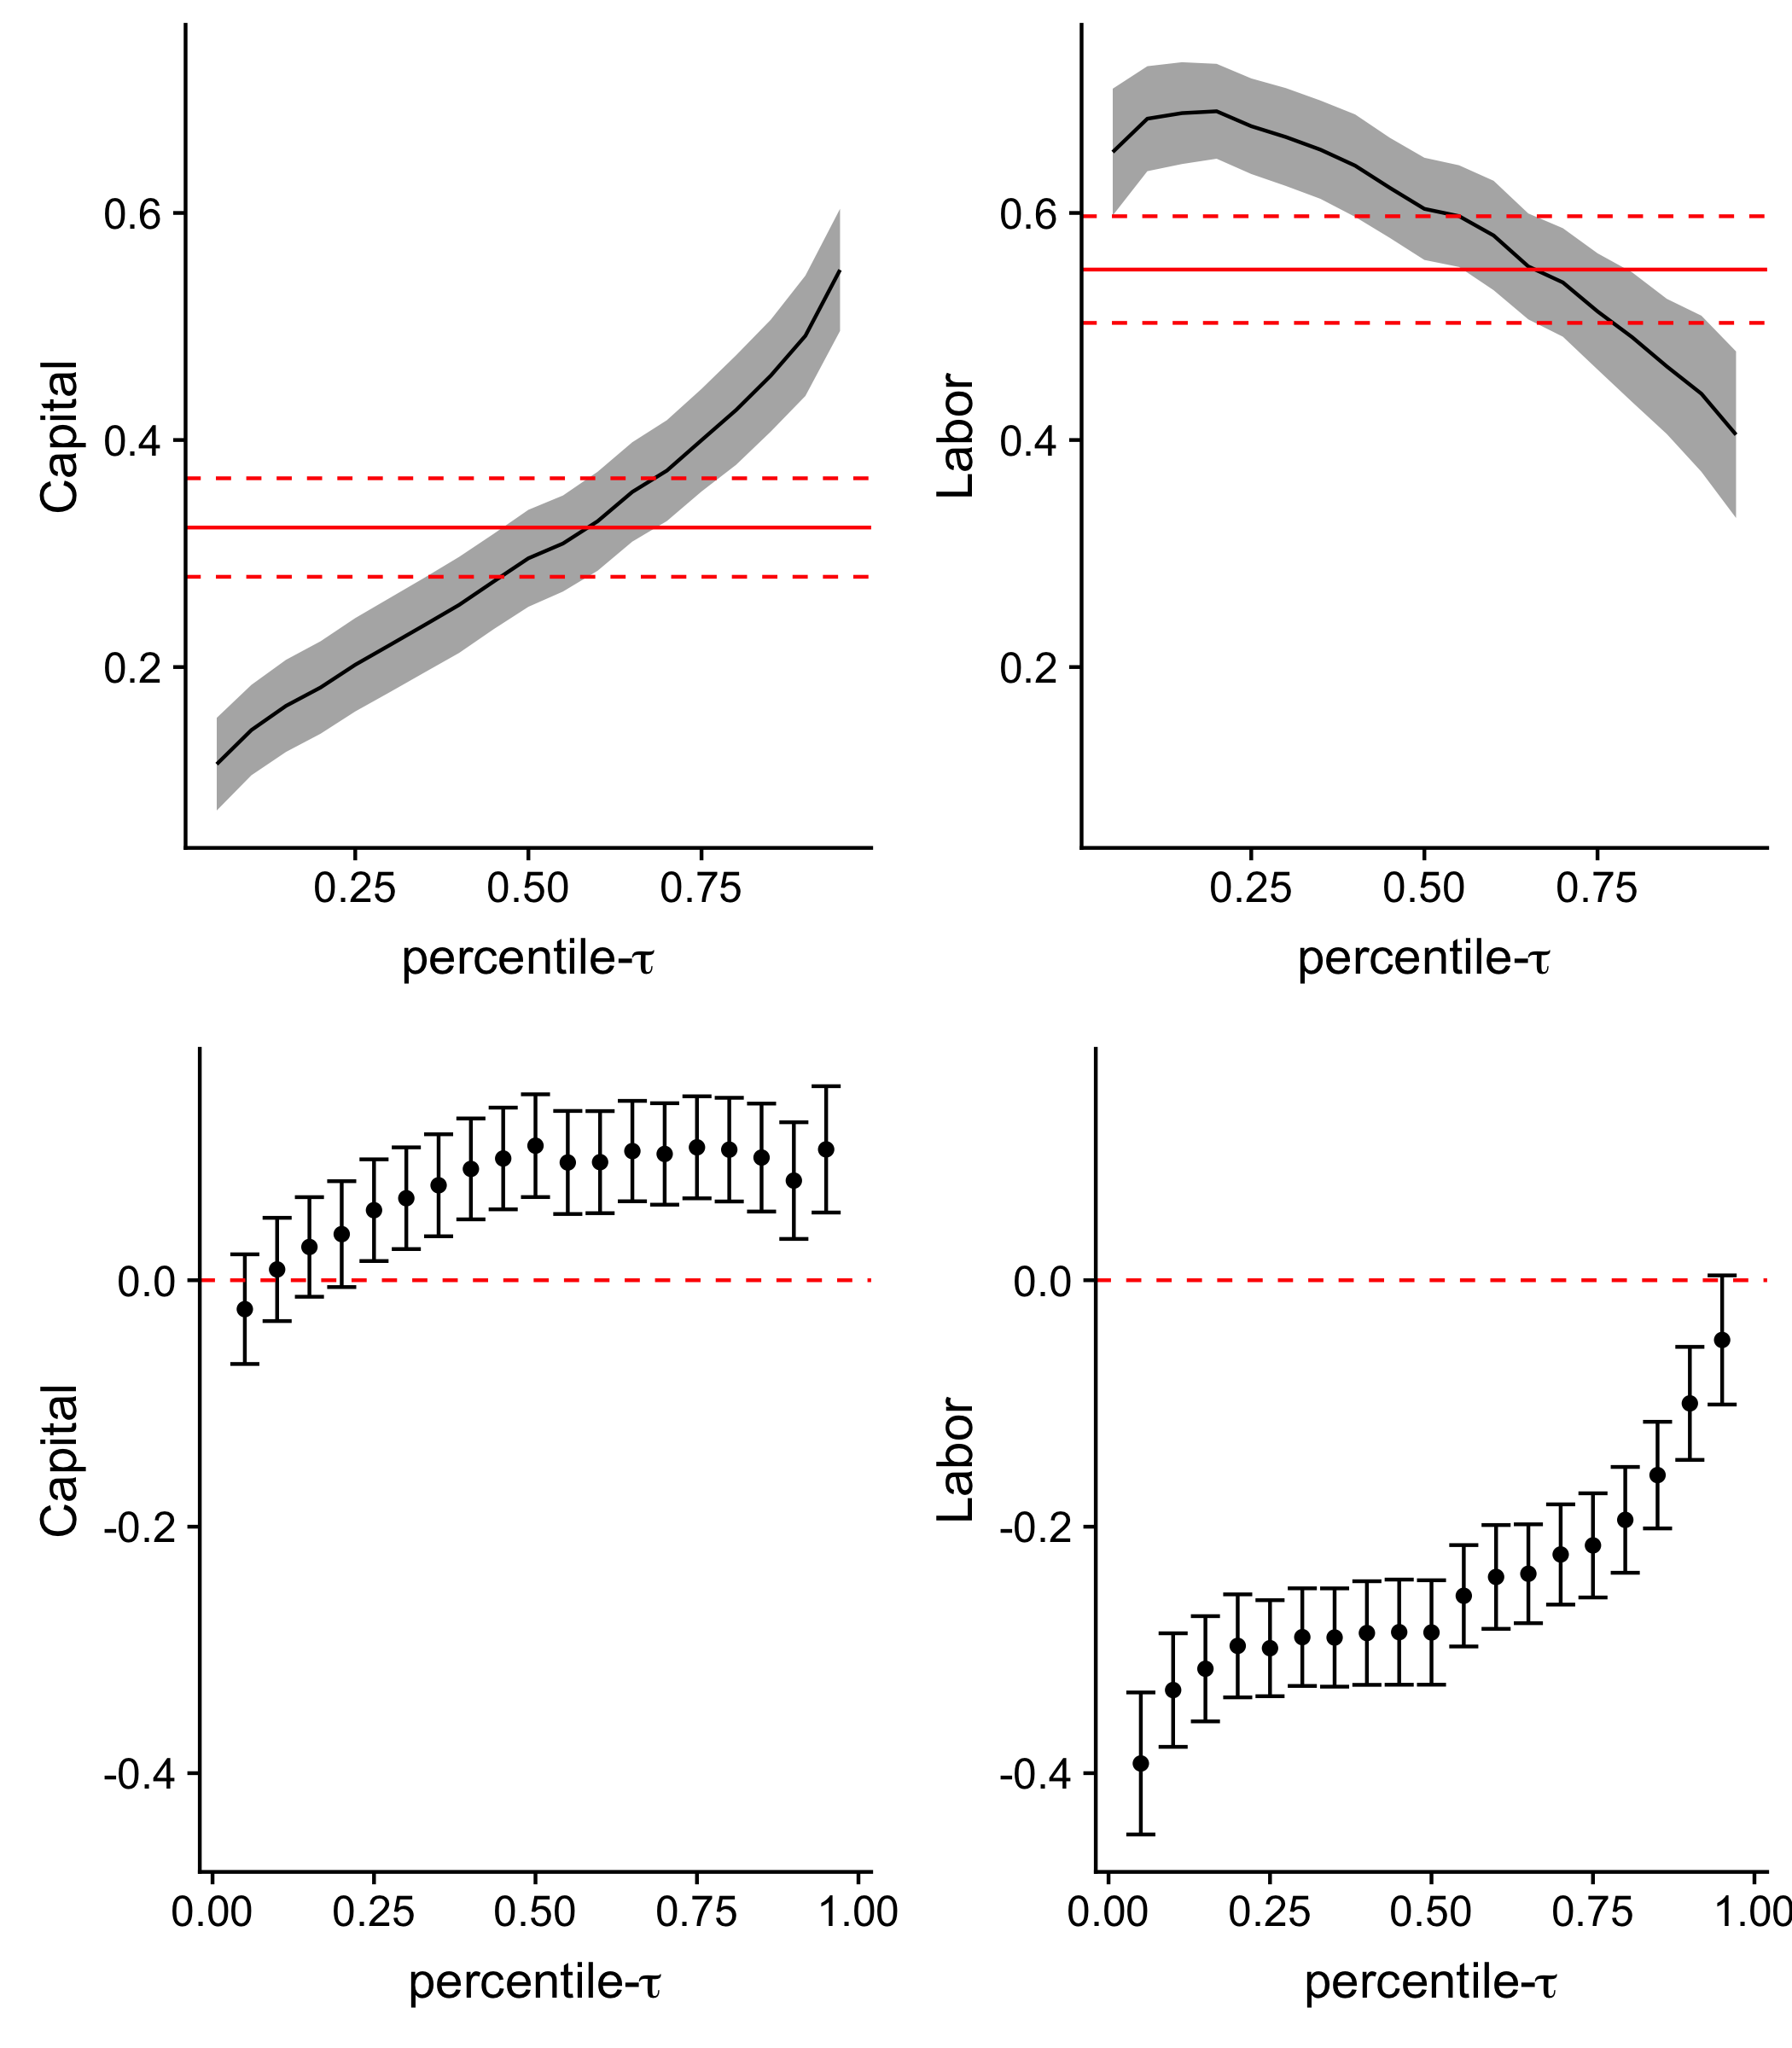
\includegraphics[width=8cm, height=8cm]{Colombia/QLP_Coef_Plot_ISIC_322.png}
\caption*{\footnotesize $^{*}$Top row: Estimated values of production function coefficients and their point-wise 90\% confidence interval. Bottom row: Difference between DS and QR estimates that does not control for endogeneity and their 95\% confidence intervals.}
\label{fig:LPCOL321}
\end{figure}

\begin{figure}[H]
\centering
\caption{Estimated Coefficients of Capital and Labor for Colombia: ISIC 381}
\includegraphics[width=8cm, height=8cm]{Colombia/QLP_Coef_Plot_ISIC_381.png}
\caption*{\footnotesize $^{*}$Top row: Estimated values of production function coefficients and their point-wise 90\% confidence interval. Bottom row: Difference between DS and QR estimates that does not control for endogeneity and their 95\% confidence intervals.}
\label{fig:LPCOL381}
\end{figure}

\begin{figure}[H]
\centering
\caption{Estimated Coefficients of Capital and Labor for Colombian Manufacturing Plants}
\includegraphics[width=8cm, height=8cm]{Colombia/QLP_Coef_Plot_ISIC_All.png}
\caption*{\footnotesize $^{*}$Top row: Estimated values of production function coefficients and their point-wise 90\% confidence interval. Bottom row: Difference between DS and QR estimates that does not control for endogeneity and their 95\% confidence intervals.}
\label{fig:LPCOLall}
\end{figure}

\begin{figure}[H]
\centering
\caption{DS and LP Estimates of Log Total Factor Productivity}
\includegraphics[width=11cm]{Colombia/QLP_TFP_Plot.png}
\caption*{\footnotesize $^{*}$Estimated distributions of TFP from the DS estimator for $\tau \in \{0.1, 0.5, 0.9\}$ and those from  the LP estimator.}
\label{fig:LPTFPDens}
\end{figure}

\begin{figure}[H]
\centering
\caption{Colombian Productivity Over Time}
\includegraphics[width=11cm]{Colombia/QLP_TFPgrowth_Plot.png}
\caption*{\footnotesize $^{*}$Estimated average productivity (in levels) over time for Colombia. Base year productivity is set to 100.}
\label{fig:LPCOLpgrowth}
\end{figure}

\begin{table}[H]
\centering
\caption{Productivity Differentials for Colombian Manufacturing Plants using DS}
\small
\begin{tabular}{cccccccc}
  \hline\hline & & \multicolumn{2}{c}{Exports}  & \multicolumn{2}{c}{Imports} & \multicolumn{2}{c}{Advertisements} \\ \cmidrule(lr){3-4} \cmidrule(lr){5-6} \cmidrule(lr){7-8}ISIC & $\tau$ & Coef. & s.e & Coef. & s.e & Coef. & s.e \\ 
  \hline
311 & 0.10 & 0.041 & 0.0144 & 0.087 & 0.0167 & 0.064 & 0.0144 \\ 
   & 0.25 & 0.036 & 0.0139 & 0.084 & 0.0152 & 0.063 & 0.0134 \\ 
   & 0.50 & 0.032 & 0.0137 & 0.082 & 0.0141 & 0.063 & 0.0126 \\ 
   & 0.90 & 0.015 & 0.0135 & 0.069 & 0.0124 & 0.056 & 0.0113 \\ 
  322 & 0.10 & 0.049 & 0.0126 & 0.092 & 0.0147 & 0.073 & 0.0117 \\ 
   & 0.25 & 0.046 & 0.0118 & 0.086 & 0.0141 & 0.066 & 0.0115 \\ 
   & 0.50 & 0.044 & 0.0114 & 0.079 & 0.0140 & 0.060 & 0.0116 \\ 
   & 0.90 & 0.034 & 0.0106 & 0.060 & 0.0142 & 0.043 & 0.0120 \\ 
  381 & 0.10 & 0.118 & 0.0226 & 0.155 & 0.0246 & 0.142 & 0.0227 \\ 
   & 0.25 & 0.114 & 0.0221 & 0.151 & 0.0238 & 0.137 & 0.0220 \\ 
   & 0.50 & 0.109 & 0.0219 & 0.146 & 0.0233 & 0.131 & 0.0216 \\ 
   & 0.90 & 0.089 & 0.0210 & 0.126 & 0.0216 & 0.108 & 0.0202 \\ 
  All & 0.10 & 0.074 & 0.0059 & 0.129 & 0.0058 & 0.101 & 0.0049 \\ 
   & 0.25 & 0.068 & 0.0056 & 0.120 & 0.0056 & 0.094 & 0.0047 \\ 
   & 0.50 & 0.061 & 0.0053 & 0.111 & 0.0055 & 0.088 & 0.0046 \\ 
   & 0.90 & 0.042 & 0.0048 & 0.086 & 0.0055 & 0.068 & 0.0044 \\ 
   \hline
\end{tabular}
\caption*{\footnotesize $^{*}$Standard errors are obtained using bootstrap with 500 replications. Log(TFP) is regressed on log(Exports), log(Imports), and log(Advertisements).}
\label{QLPCOLTFPP}
\end{table}

\begin{table}[H]
\centering
\caption{Productivity Differentials for Colombian Manufacturing Plants using LP}
\small
\begin{tabular}{ccccccc}
  \hline\hline & \multicolumn{2}{c}{Exports}  & \multicolumn{2}{c}{Imports} & \multicolumn{2}{c}{Advertisements} \\ \cmidrule(lr){2-3} \cmidrule(lr){4-5} \cmidrule(lr){6-7}ISIC & Coef. & s.e & Coef. & s.e & Coef. & s.e \\ 
  \hline
311 & 0.029 & 0.0135 & 0.079 & 0.0139 & 0.061 & 0.0124 \\ 
  322 & 0.043 & 0.0114 & 0.078 & 0.0139 & 0.060 & 0.0115 \\ 
  381 & 0.108 & 0.0216 & 0.145 & 0.0230 & 0.130 & 0.0212 \\ 
  All & 0.060 & 0.0053 & 0.109 & 0.0055 & 0.086 & 0.0046 \\ 
   \hline
\end{tabular}
\caption*{\footnotesize $^{*}$Standard errors are obtained using bootstrap with 500 replications. Log(TFP) is regressed on log(Exports), log(Imports), and log(Advertisements).}
\label{LPCOLTFPP}
\end{table}


















\end{appendices}




\end{document}